\chapter{Evaluation procedure and discussion of results}
\label{chap:analysis}

In the previous Chapter, we built a reinforcement learning environment with the use of the components which were described earlier, in Chapter \ref{chap:preliminaries}.
The environment facilitates the simulation of order placement on historical order books of the type described in Chapter \ref{chap:data}.
Furthermore, two agents were introduced: a Q-Learner which learns on private variables; and a Deep Q-Network which learns on market variables.

The aim of this chapter is to make use of this setup and to run simulations, thereby observing whether or not reinforcement learning is indeed capable of optimizing the placement of limit orders.
Therefore, a comprehensive evaluation procedure will be introduced that  measures the capabilities of the reinforcement learning agents.
Throughout this process, real world historical order books will be drawn upon, as well as artificially created order books, where the latter define distinct price trends and eliminate the noise present in real market data.
We first outline the steps of the evaluation procedure.
Subsequently, the real world data sets chosen and their use within the reinforcement learning setup will be described.
Finally, we will proceed evaluation steps with our agents.
Accordingly, this chapter will seek to quantify the effectiveness of deep reinforcement learning and its use of the market features previously constructed.

\section{Explanation of the evaluation procedure}
\label{sec:analysis-procedure}
This section explains the evaluation procedure that will be elaborated in the following sections of this chapter. From our analysis of the same, we will aim to formulate a statement that expresses the capabilities of optimizing limit order placement with reinforcement learning and the use of raw market data.
The evaluation steps will proceed chronologically, as follows:
\begin{description}
    \item[Empirical investigation: ]
    Section \ref{sec:eval-empirical} investigates the reinforcement learning environment empirically by simulating an agent's behaviour that places buy and sell orders for a range of limit levels.
    This will provide knowledge about the limitations of the potential optimization possibilities within the given data set and how well we can expect the reinforcement learners to perform.
    More precisely, we determine the \textit{expected returns} for (1) the optimally chosen limit order and (2) an immediate purchase or sale by using a market order.
    
    \item[Q-Learning agent policy: ]
    In Section \ref{sec:eval-qlearn}, we will make an attempt to build an order placement policy based on private variables only, by using the Q-Learner.
    This will provide insights into the performance of a naive reinforcement learner and serve as a benchmark for the following simulations proceeded in which we consider market variables.
    Thereby, we observe the \textit{average reward} achieved by the Q-Learning agent that uses private variables.

    \item[DQN agent policy: ]
    Section \ref{sec:eval-dqn} applies market variables to the DQN agent.
    Hereby, we will make use of Feature I: the price and size of historical orders as described in Chapter \ref{chap:data} (Section \ref{sec:data-feature-1}); as well as Feature II: the price and size of historical trades (described in Section \ref{sec:data-feature-2}).
    As in the previous evaluation step, we will find the average rewards produced by the agent.
    More precisely, we determine the average rewards for the DQN agent with the use of private variables and (1) historical orders or (2) historical trades.

    \item[DQN agent limitations: ]
    Section \ref{sec:eval-dqn-limitations} aims to determine the capabilities and limitations of the DQN agent in greater detail.
    We will investigate the actions selected by the agent in order to determine the agent's limitations.
    In addition, we apply the agent to an environment which is equipped with an artificially generated order book and will enable us to determine to which extent the agent is able to learn from certain price trends.
    The results achieved in this evaluation step are (1) \textit{the discovery} of situations where the DQN agent does not perform as expected and (2) the \textit{average reward} achieved by using order books that follow an artificially created trend (downwards and sine curve).
\end{description}
With the results obtained throughout this evaluation, we will be able to determine and quantify the extent to which deep reinforcement learning can optimize limit order placement; we will also be able to give reasons for its limitations.

\section{Data sets and their usage in the reinforcement learning setup}
\label{sec:analysis-data-sets}
We have selected two $\sim$30 minute samples of historical order book recordings for the experiments in this chapter.
One of the reasons for choosing two very different data sets is to determine the ability of the learners to react to a variety of market situations.
In addition, as explained in the following section, the expected return of a learner for buying and selling assets heavily depends on the market price movements and therefore the behaviour is expected to be different for the data sets in use.
More precisely, \textit{data set I}, as shown in Figure \ref{fig:sample-down-price}), is a downward trend (indicated by the bid/ask mid-price) and consists of 1132 order book states with an overall duration of 1681.8 seconds, resulting in 0.67 states per second.
In contrast, \textit{data set II}, as shown in Figure \ref{fig:sample-up-price}, consists of 1469 order book states with an overall duration of 1746.0 seconds, resulting in 0.84 states per second, which indicates that there was slightly more pressure in terms of orders placed and canceled in this data set.
When reinforcement learning is applied, the data sets are split with ratio $2:1$, resulting in a training set of $\sim$20 minutes and a test set of $\sim$10 minutes.
Although more than two data sets would produce a more generalized outcome of this evaluation, this was computationally not feasible within this work.
\begin{figure}[H]
    \centering
    \begin{subfigure}[b]{0.45\textwidth}
        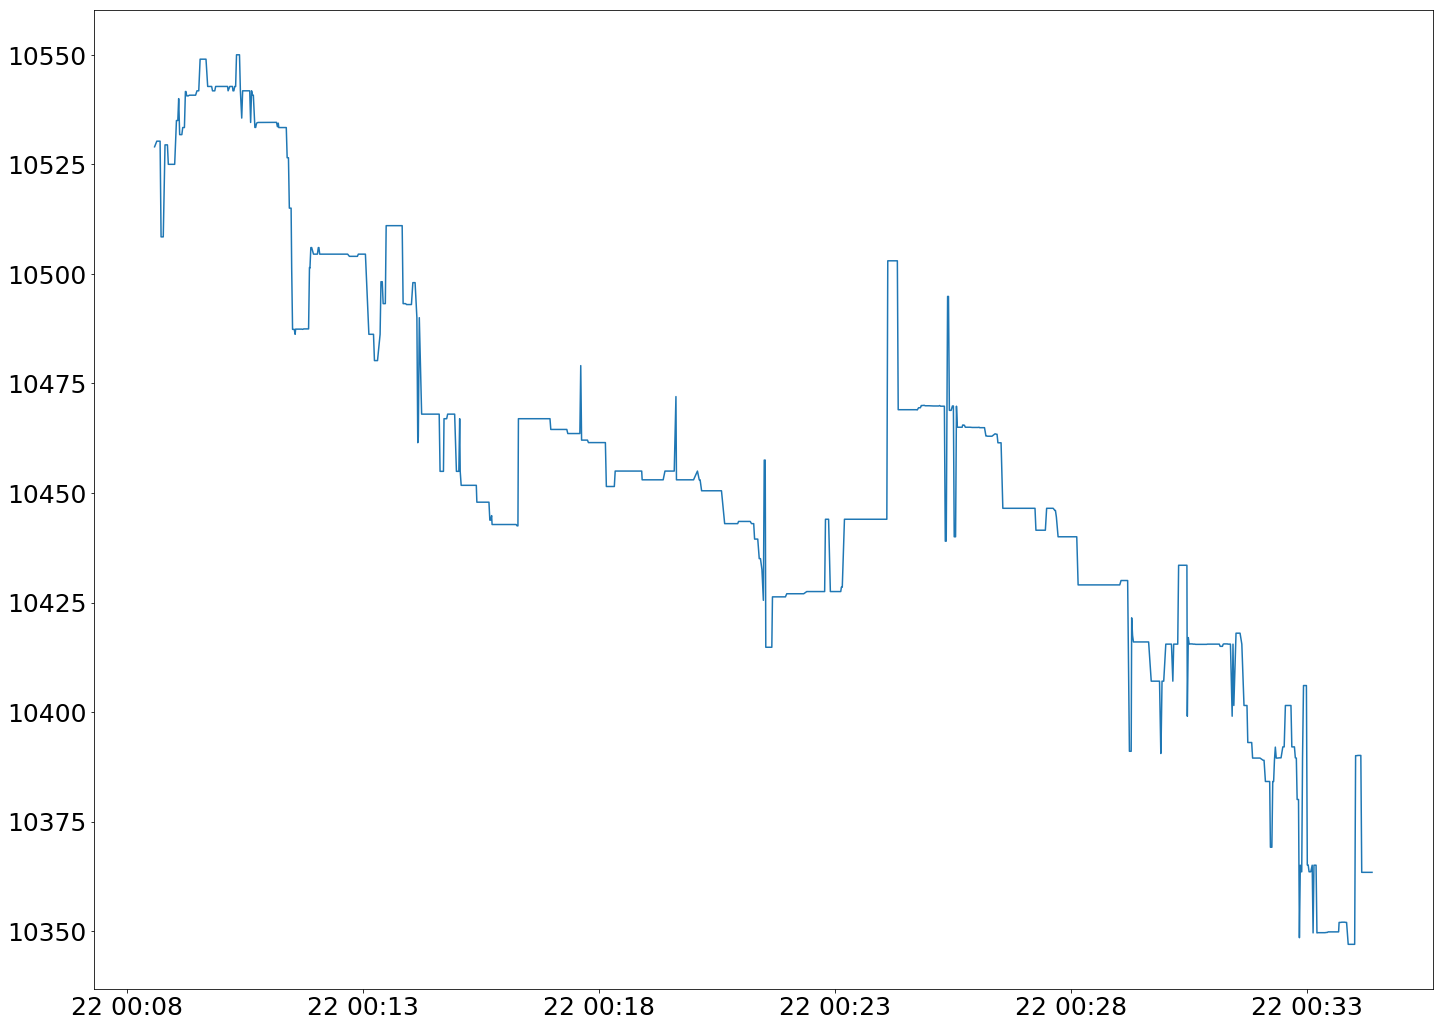
\includegraphics[width=\textwidth]{sample-down-price}
        \caption{30 minute downwards trend}
        \label{fig:sample-down-price}
    \end{subfigure}
    \begin{subfigure}[b]{0.45\textwidth}
        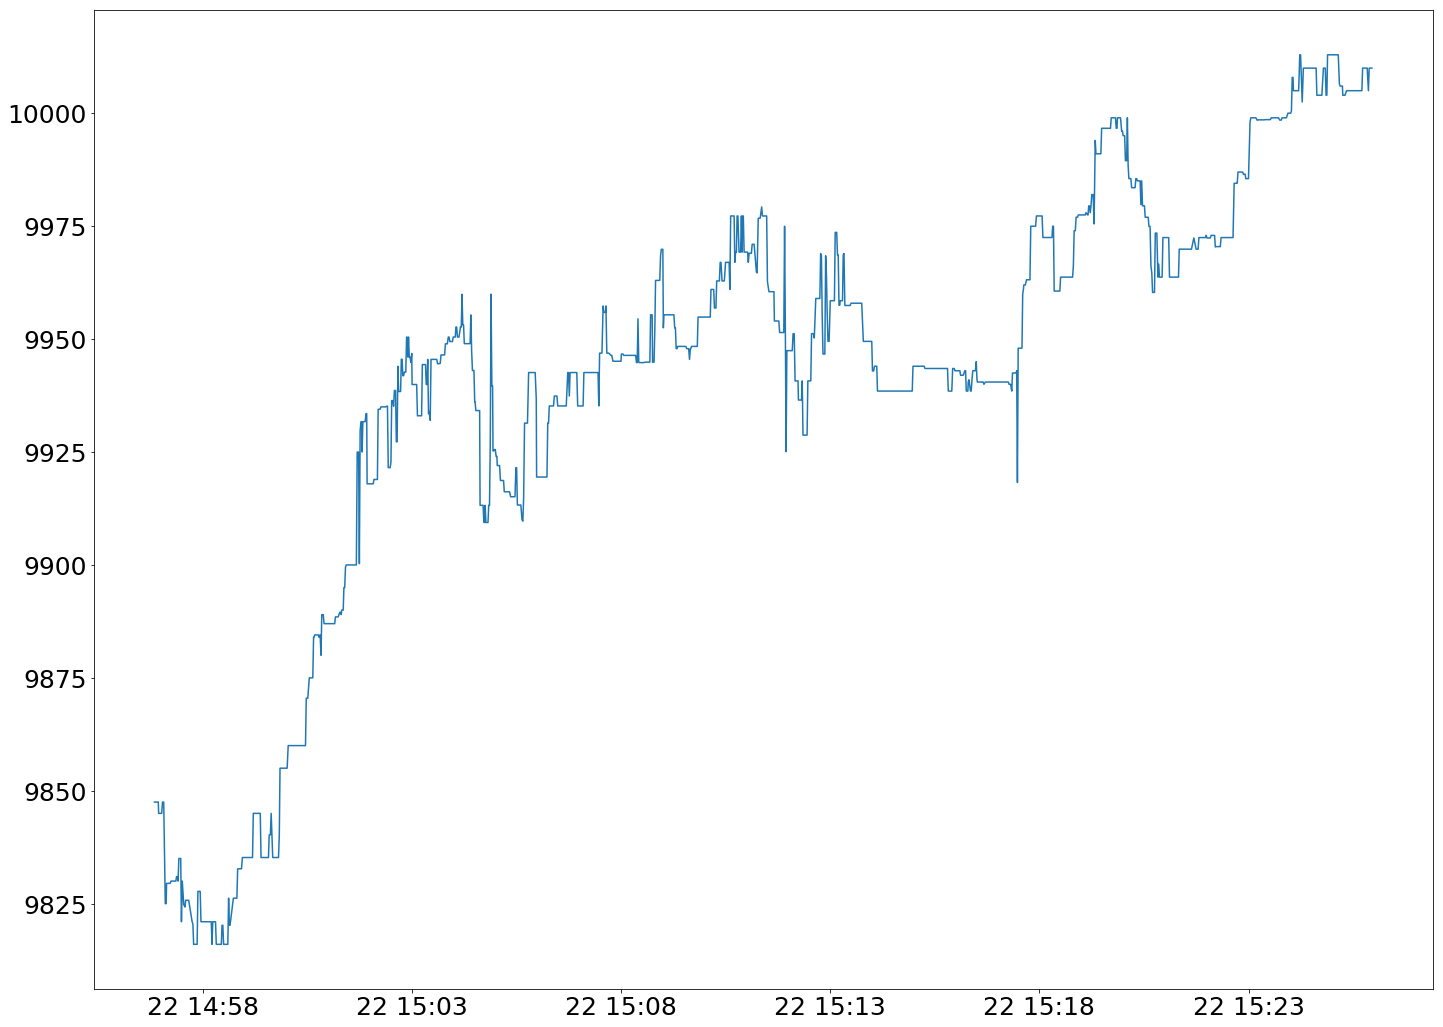
\includegraphics[width=\textwidth]{sample-up-price}
        \caption{30 minute upwards trend}
        \label{fig:sample-up-price}
    \end{subfigure}
    \caption{Bid/ask mid-price of 30 minute order book recordings.}
    \label{fig:sample-price}
\end{figure}

As explained in Chapter \ref{chap:setup}, the historical data sets are not maintained by the reinforcement learning agents directly but instead by the reinforcement learning environment.
The environment provides an observation state $O$, derived from the data set, to an agent, after which the agent decides to take an action $a$ in the form of a limit level.
In turn, the environment prices the order at the received price level and returns the evaluated reward $r$ and the next observation state $O$ to the agent.
In this way, the agent can simulate the placement of limit orders in such a way that, within the given time horizon $H$, the inventory can be either bought or sold.
For each \textit{epoch} an agent processes, one order, with a specified inventory and time horizon, is defined and is to be filled.
Therefore, the reinforcement learning environment selects, for each epoch the agent initiates, a range of order book states which form the given time horizon $H$ within which the agent is supposed to complete an order.
\begin{figure}[H]
    \centering
    \makebox[\linewidth]{
        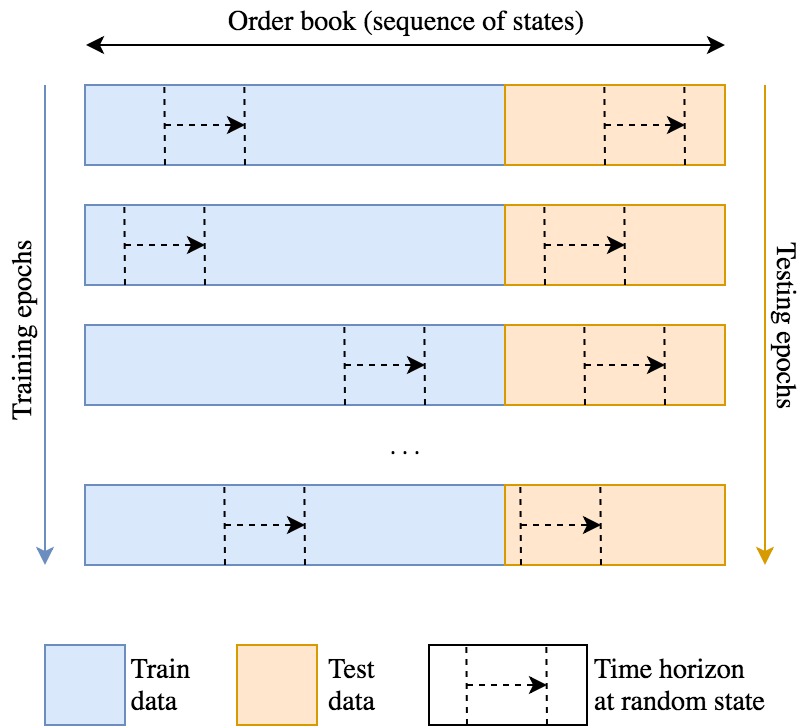
\includegraphics[width=8cm]{images/evaluation-orderbook.png}
    }
    \caption{Order placement training and testing on an order book data set.}
    \label{fig:eval-orderbook-window}
\end{figure}
Figure \ref{fig:eval-orderbook-window} illustrates this process.
A randomly-chosen order book state will define the beginning of the time horizon and the set of order book states that will fall into this window.
This is very crucial since the states within this time horizon and the set of states, not only will lead to the observation states received by the agent, but also will determine the outcome of the matching process.
More precisely, for each step the agent takes, a consecutive sequence of order book states (with time stamp difference of $\Delta{t}$) is considered by the match engine, as explained in the previous chapter in Section \ref{setup:parameters}.
This process is identical for testing, except that the underlying data is different and the agent will not learn from the epochs to be proceeded during testing and instead will report the achieved rewards.

\section{An empirical investigation of the reinforcement learning environment}
\label{sec:eval-empirical}
In this section, the relationship between the limit order placement and the received return will be investigated.
This method was demonstrated in the related work Section \ref{sec:related-execution-behaviour} and was taken to empirically evaluate the reinforcement learning environment.
Therefore, we will simulate an agent that submits actions in order to buy and sell shares at every possible limit level and records the immediate returns it receives.
A return is defined as the difference between the market price prior to the order placement and the volume- weighted average price (VWAP) paid or received, as stated in Eq. \ref{setup:reward}.
Hence, we will gain an understanding of the estimated rewards of limit order placement in the historical data set in use.
In addition, these results will set a benchmark for the reinforcement learners to come.

We will now describe the setup of this investigation.
We will investigate the rewards of limit orders placed on progressively increasing time horizons, from 10 seconds to 100 seconds, and thereby observe the importance of the action chosen by the agents in order to buy or sell assets, in accordance with the length of the time horizon.
For each time horizon, we will place (e.g. cross-validate) 100 orders of size 1.0 BTC at the beginning of this time horizon whose beginning is defined by a randomly-chosen order book state. 
A market order follows for the remainder of shares (if any) once the time horizon is consumed.
The expected return will then be derived from the average of the received returns of these 100 orders.
This process will be repeated across a range of 201 actions $A$ that correspond to the limit levels $-100...100$ with step size $\Delta{a} = \$0.10$, resulting in orders priced in the range of $p_m-10 \ \dots \ p_m+10$, whereas $p_m$ is the market price before the order was placed.
The limit levels will be chosen broadly in order to retrieve understanding about the outcome of a variety of possible actions.
As a result, a total of 20,100 orders will be submitted for each time horizon defined.
This procedure will be undertaken for both data sets I and II.

\subsection{Order placement behavior on data set I}
For data set I, where the market sees a downwards trend, the assumption is as follows:
We expect buy orders to result in better returns when placed deep in the order book, in other words, on orders that have a highly negative limit level ($a<0$).
Since the price tends to fall, the assumption is that an agent is able to buy at a lower price as time passes.
Therefore, the longer the time horizon, the lower the limit level that can still be chosen in order to execute the full amount of shares.
In contrast, we expect sell orders to provide better returns when the agent crosses the spread with a positive limit level ($a>0$).
The assumption is that, in a falling market, it is unlikely that market participants are willing to buy at higher prices and therefore the agent must place sell orders higher in the book in order to sell immediately.
Otherwise, the longer the time horizon, the less return an agent would retrieve as the market order, that is submitted if the order has not been filled, becomes costly.
This investigation is shown in Figure \ref{fig:behvaiour-down} for time horizons of 10, 30, 60 and 100 seconds.
The x-axis indicates the placement of the order at limit levels ranging from $a=-100$ to $a=+100$ and the y-axis indicates the average return received.

With a time horizon of only 10 seconds, the expected behavior is, however, proven wrong.
For buy orders, shown in Figure \ref{fig:behvaiour-down-10s-buy}, the returns suggest that orders be placed close to the spread, but still on the opposing side ($a=\sim{5}$).
The spike at limit level $a=\sim{-5}$ indicates that the overall best return was produced at this level. However, this comes with the risk that the orders fail to execute, which is indicated by the downward dip also close to level $\sim{-5}$.
For selling within 10 seconds, as shown in Figure \ref{fig:behvaiour-up-10s-sell}, the best return is given when crossing the spread with a positive limit level with $a=\sim{+50}$.

With an increased time horizon of a total of 30 seconds, as shown in Figures \ref{fig:behvaiour-down-30s-buy} and \ref{fig:behvaiour-down-30s-sell}, the expected behavior becomes more apparent.
Positive returns can be achieved by posting buy orders deep in the order book.
Therefore, we can expect that in this market situation, an agent would be able to partially execute the order at very low limit levels and, for the unexecuted part, a market order would follow.
The densest range of positive returns can be seen around the limit levels just below the spread.
Orders placed deeper in the book oftentimes result in slightly lower returns, which indicates that the orders were only filled partially and expensive market orders followed.
Crossing the spread causes increasingly lower returns, the more positive the limit level is chosen.
This is a result of the agents' willingness to immediately buy at an increased price.
The opposite effect occurs while selling assets.
Market orders higher in the book result in better returns than limit orders deep in the book.
Interestingly, orders which were placed very deep in the book, at limit level $\sim$-50 and below, were rewarded better than the ones close to the spread.
The most likely reasons it that a minority of orders  were partially filled at this level during the cross-validation process.

With time horizons of 60 and 100 seconds, the expected behavior of the orders is clearly apparent.
Buy orders, as shown in Figures \ref{fig:behvaiour-down-60s-buy} and \ref{fig:behvaiour-down-100s-buy}, achieve highest returns when placed very deep in the order book.
However, when placed at levels -100, the returns are slightly lower as a result of unexecuted orders which had to be completed with a following market orders.
In addition, positive limit levels become stable at these price levels since there are more sellers in the market with the extended time horizon.  Therefore, very highly placed orders result in the same return as limit orders posted only slightly above the spread.
Furthermore, placing orders very deep in the book has the same effect as when placing them just below the spread; that is, there are no traders willing to buy at such a high price and therefore market orders follow once time has passed.
\vfill
\newpage
\begin{figure}[H]
    \centering
    \begin{subfigure}[b]{0.45\textwidth}
        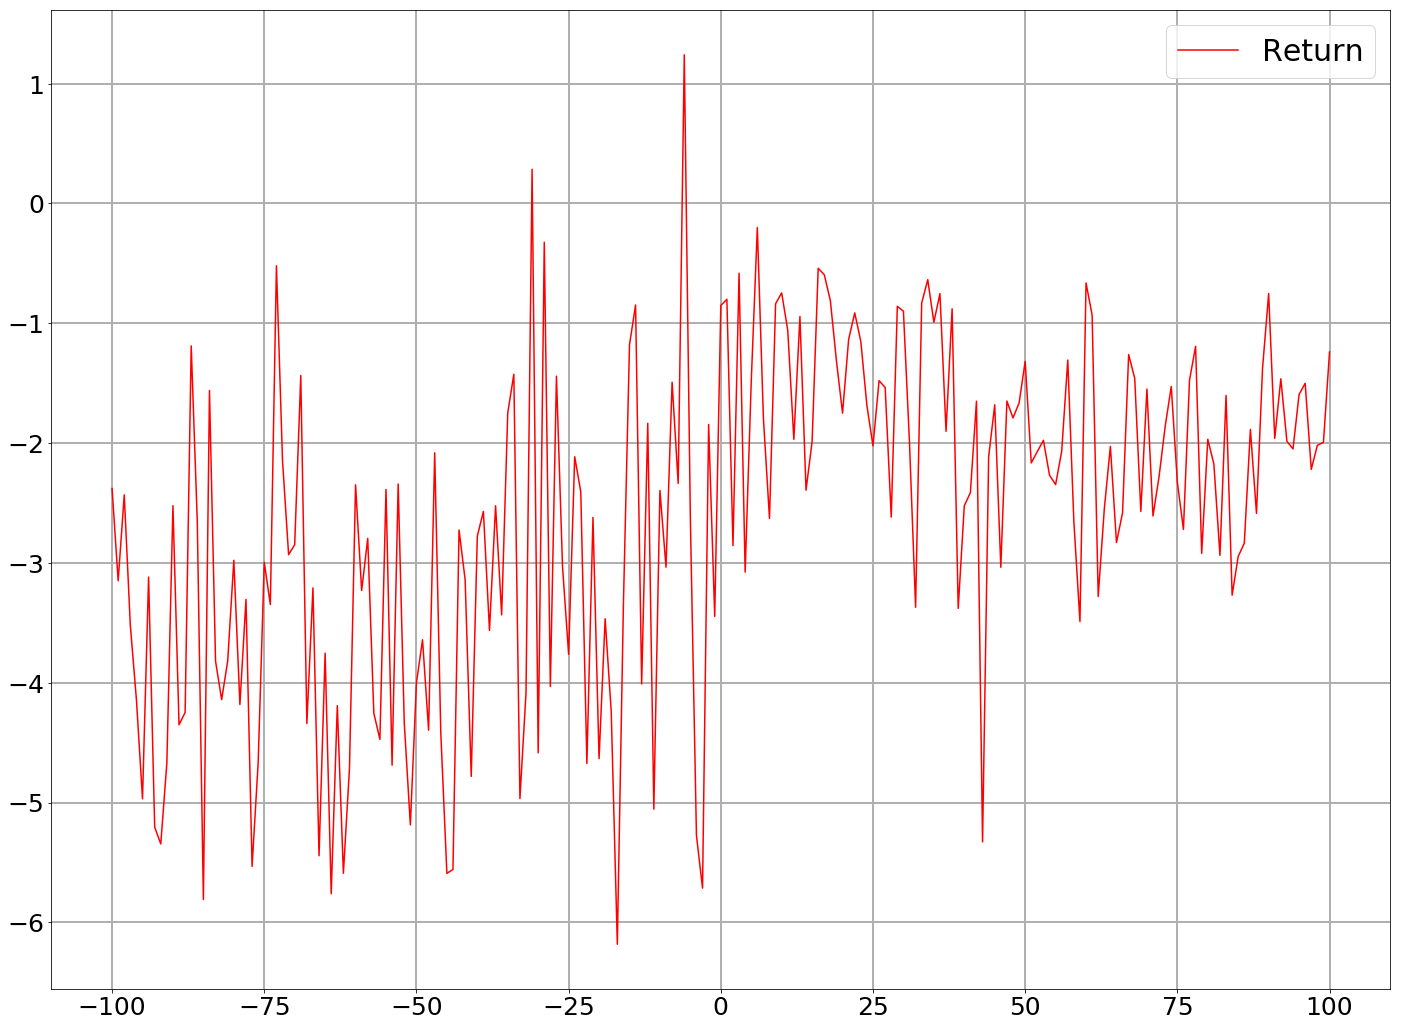
\includegraphics[width=\textwidth]{images/behaviour-10s-buy.png}
        \caption{Returns of buy orders within 10 seconds}
        \label{fig:behvaiour-down-10s-buy}
    \end{subfigure}
    \begin{subfigure}[b]{0.45\textwidth}
        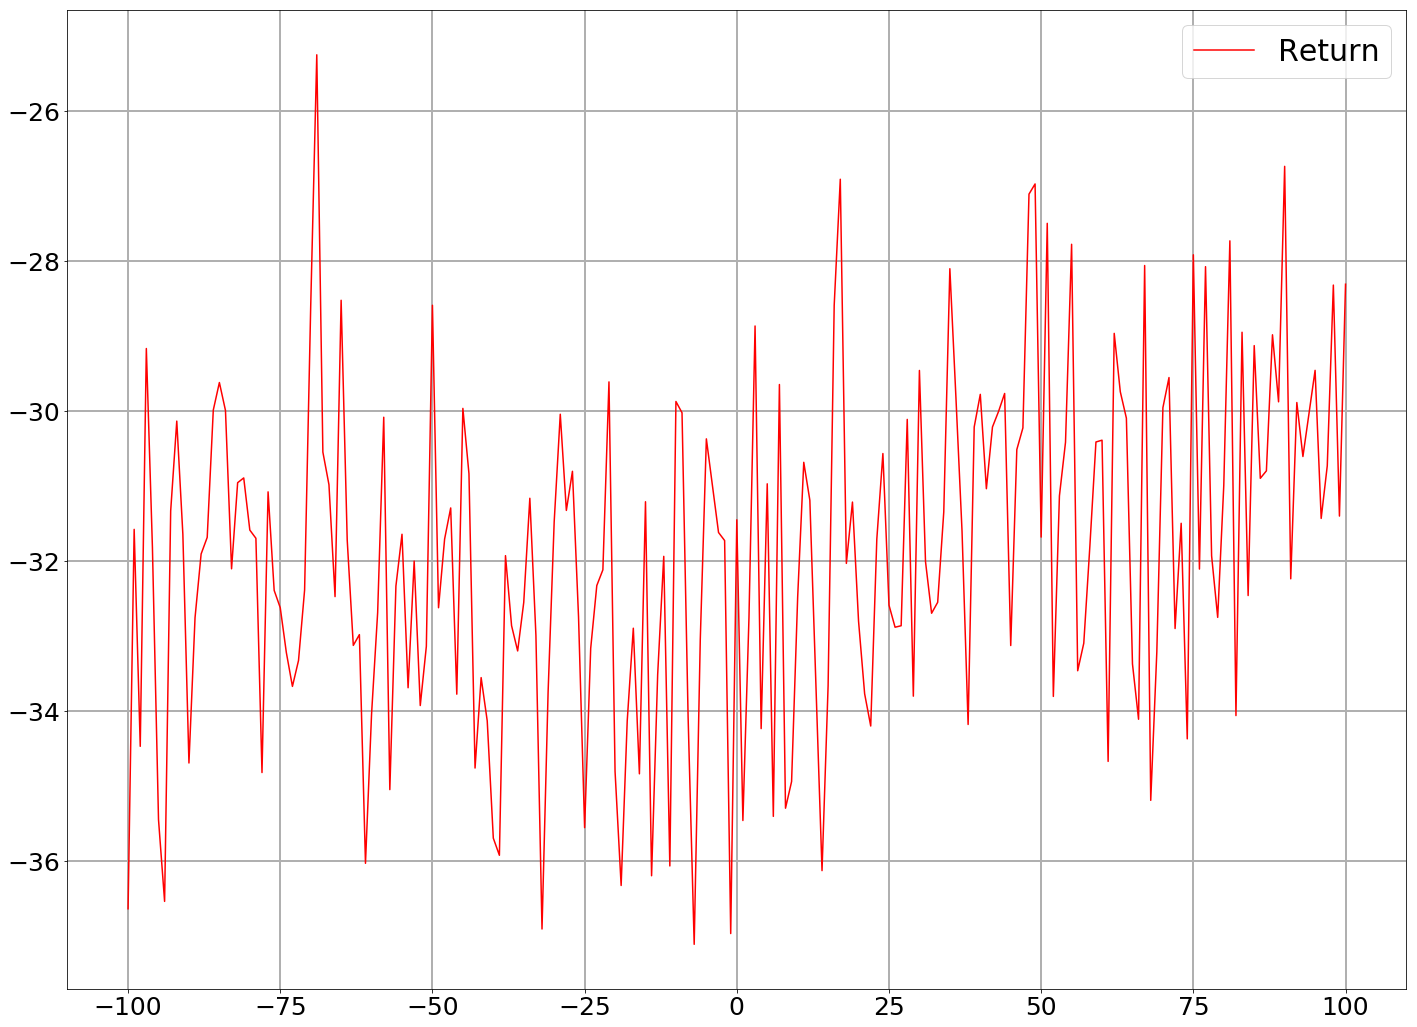
\includegraphics[width=\textwidth]{images/behaviour-10s-sell.png}
        \caption{Returns of sell orders within 10 seconds}
        \label{fig:behvaiour-down-10s-sell}
    \end{subfigure}
    \begin{subfigure}[b]{0.45\textwidth}
        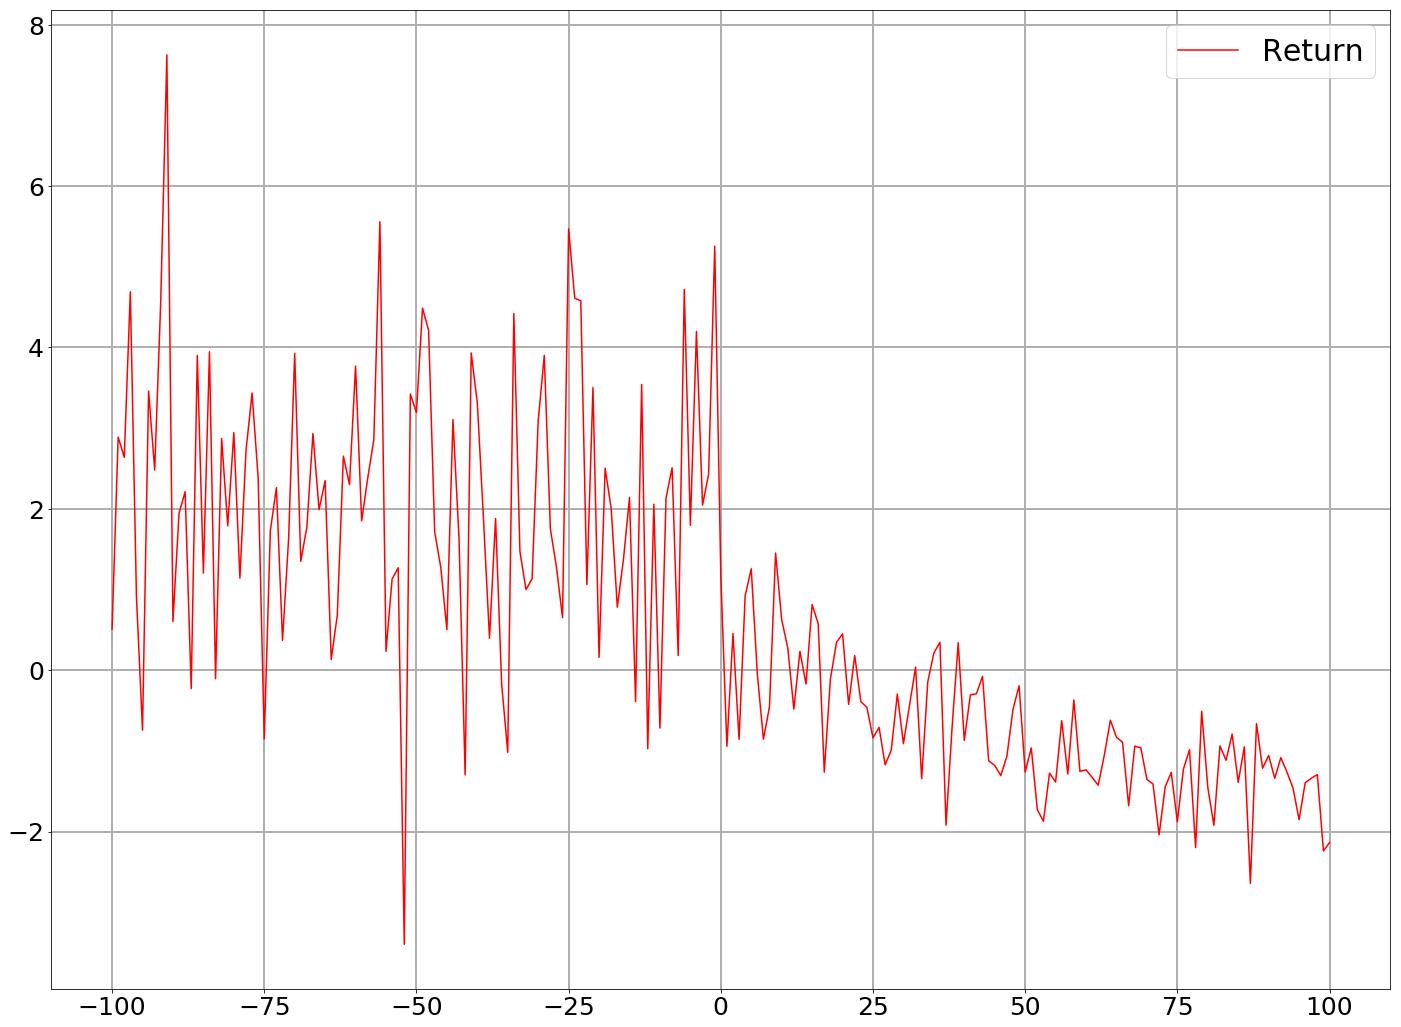
\includegraphics[width=\textwidth]{images/behaviour-30s-buy.png}
        \caption{Returns of buy orders within 30 seconds}
        \label{fig:behvaiour-down-30s-buy}
    \end{subfigure}
    \begin{subfigure}[b]{0.45\textwidth}
        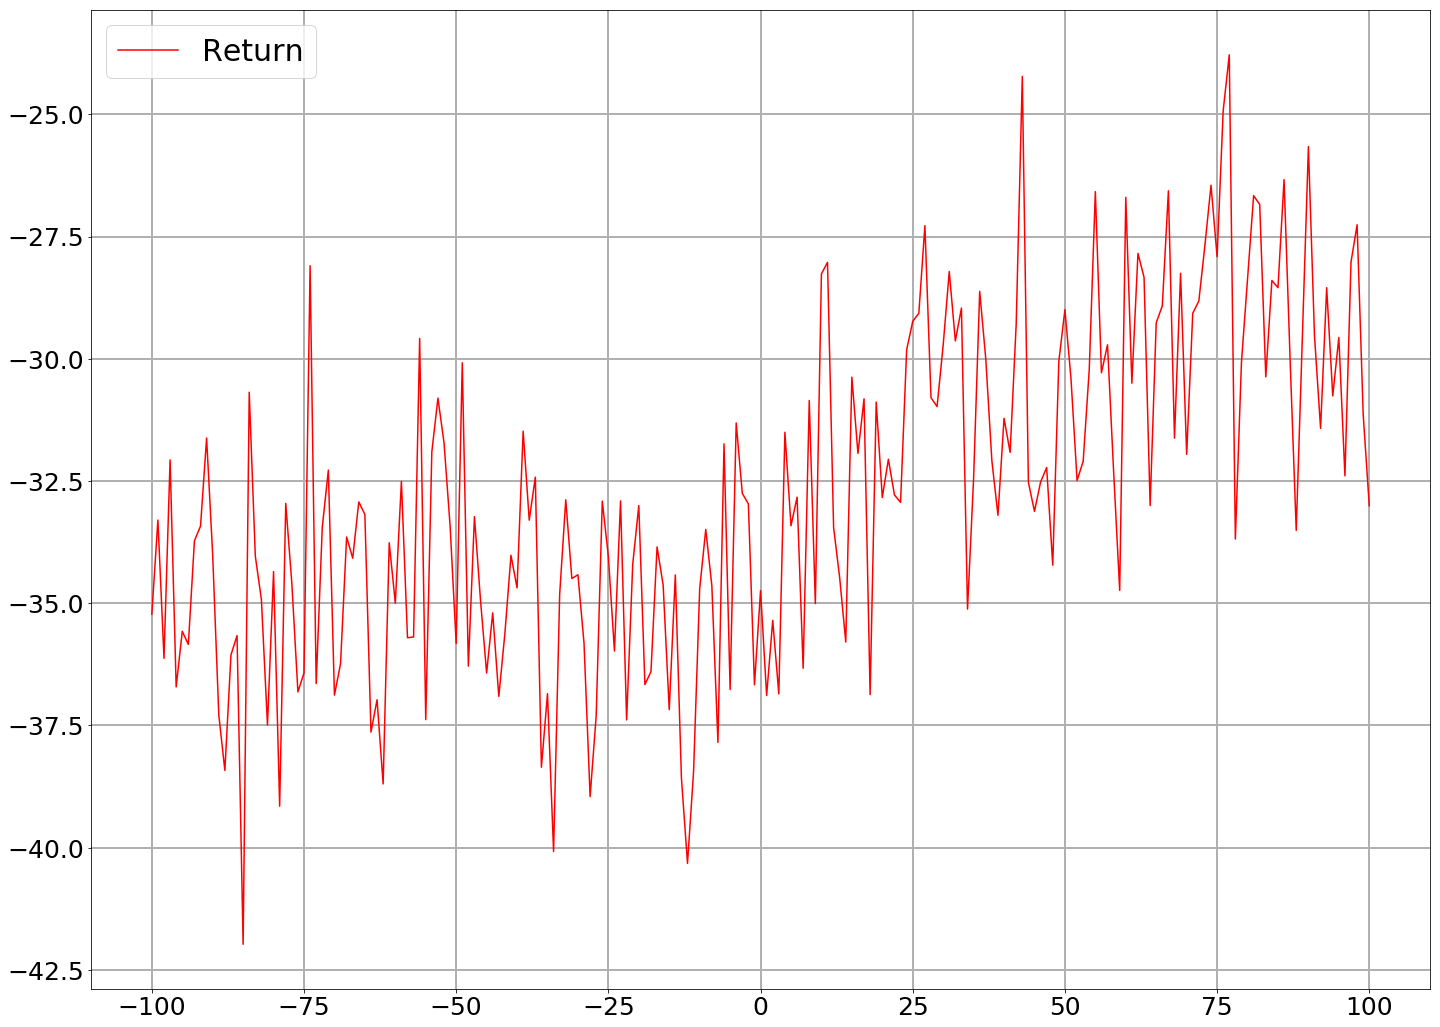
\includegraphics[width=\textwidth]{images/behaviour-30s-sell.png}
        \caption{Returns of sell orders within 30 seconds}
        \label{fig:behvaiour-down-30s-sell}
    \end{subfigure}
    \begin{subfigure}[b]{0.45\textwidth}
        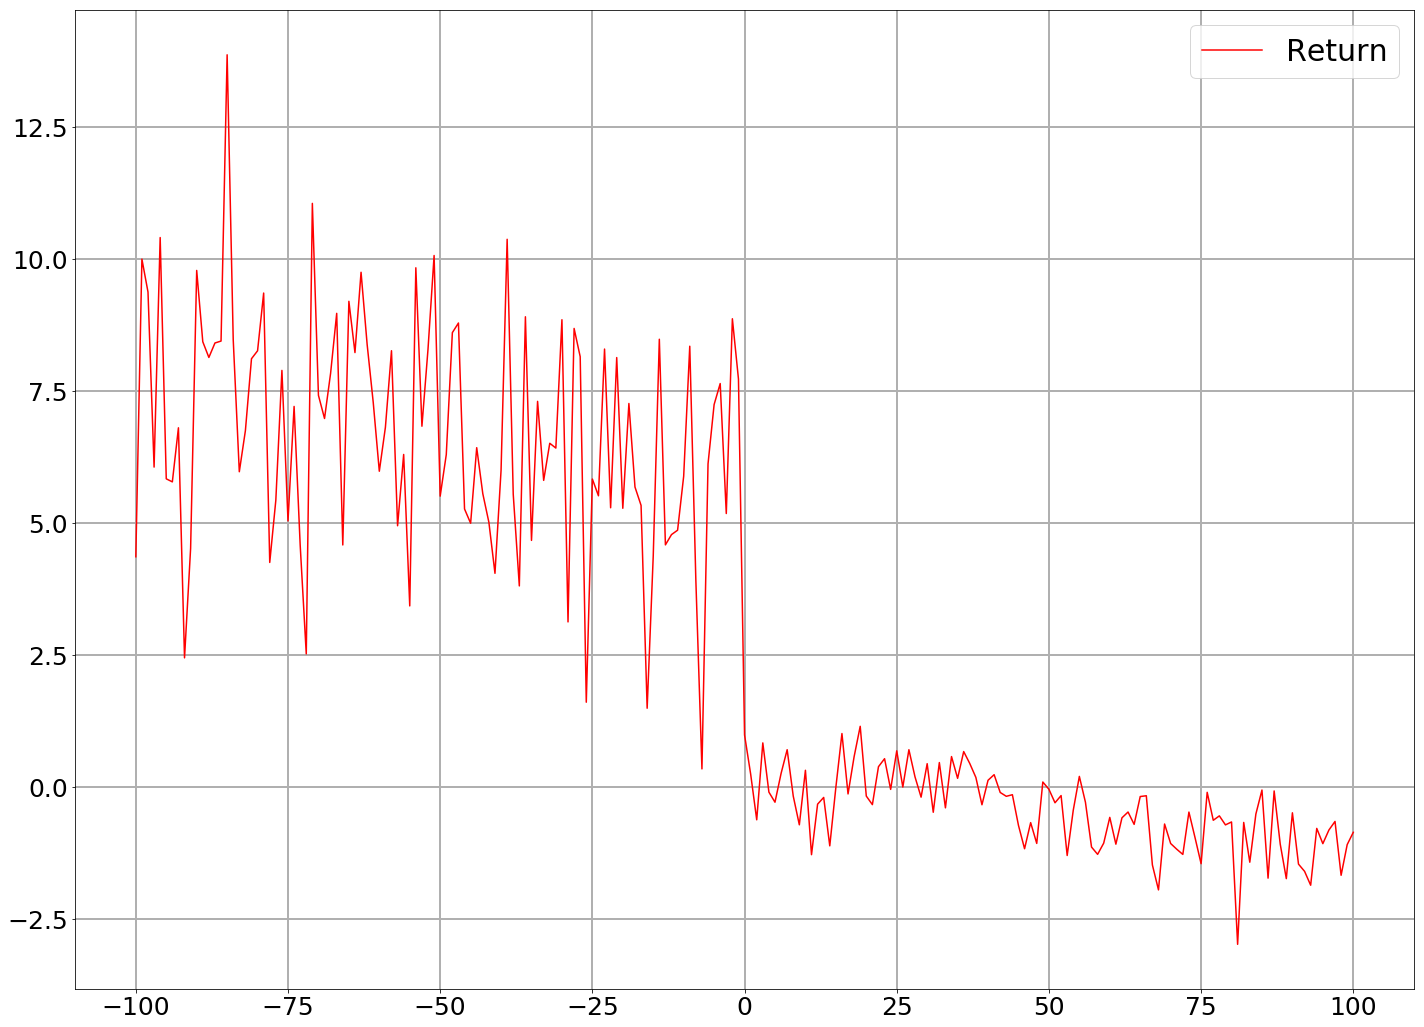
\includegraphics[width=\textwidth]{images/behaviour-60s-buy.png}
        \caption{Returns of buy orders within 60 seconds}
        \label{fig:behvaiour-down-60s-buy}
    \end{subfigure}
    \begin{subfigure}[b]{0.45\textwidth}
        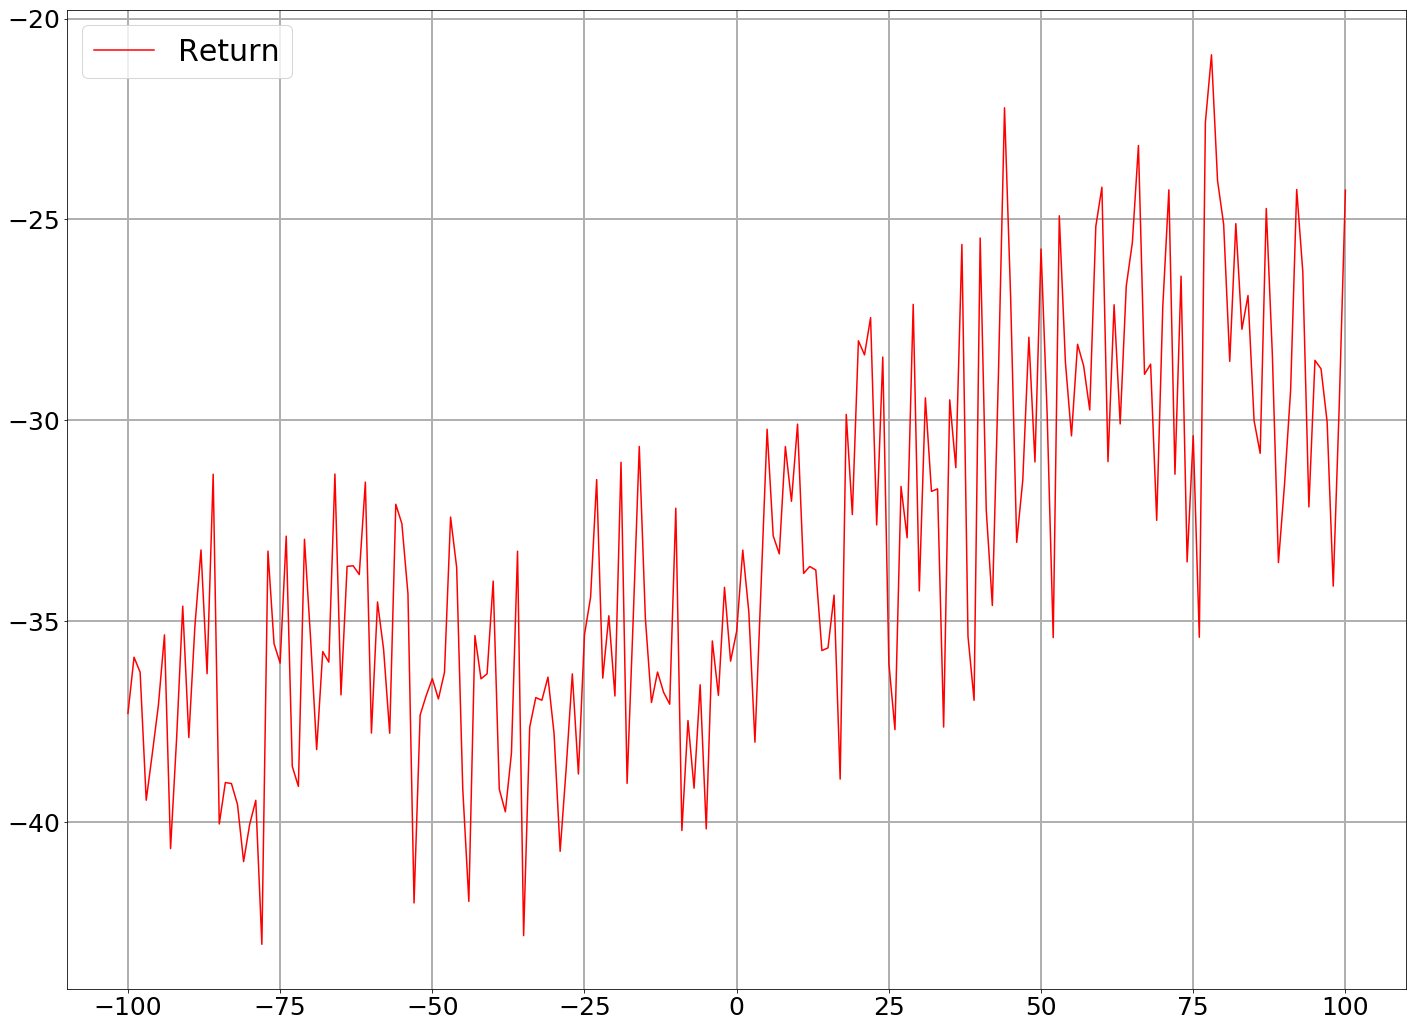
\includegraphics[width=\textwidth]{images/behaviour-60s-sell.png}
        \caption{Returns of sell orders 60 seconds}
        \label{fig:behvaiour-down-60s-sell}
    \end{subfigure}
    \begin{subfigure}[b]{0.45\textwidth}
        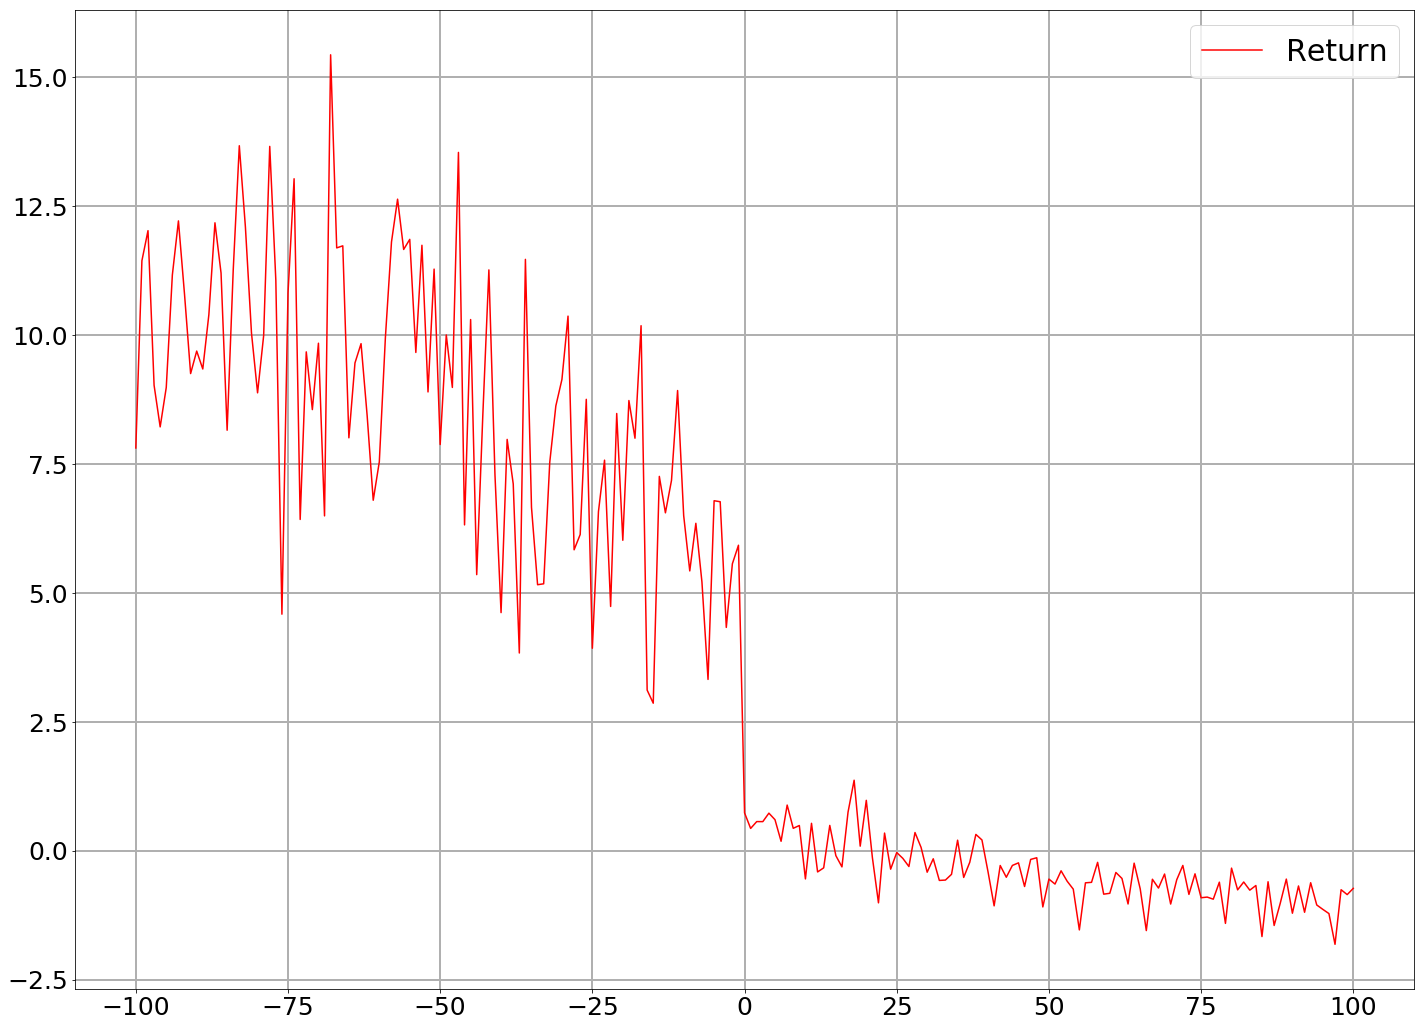
\includegraphics[width=\textwidth]{images/behaviour-100s-buy.png}
        \caption{Returns of buy orders 100 seconds}
        \label{fig:behvaiour-down-100s-buy}
    \end{subfigure}
    \begin{subfigure}[b]{0.45\textwidth}
        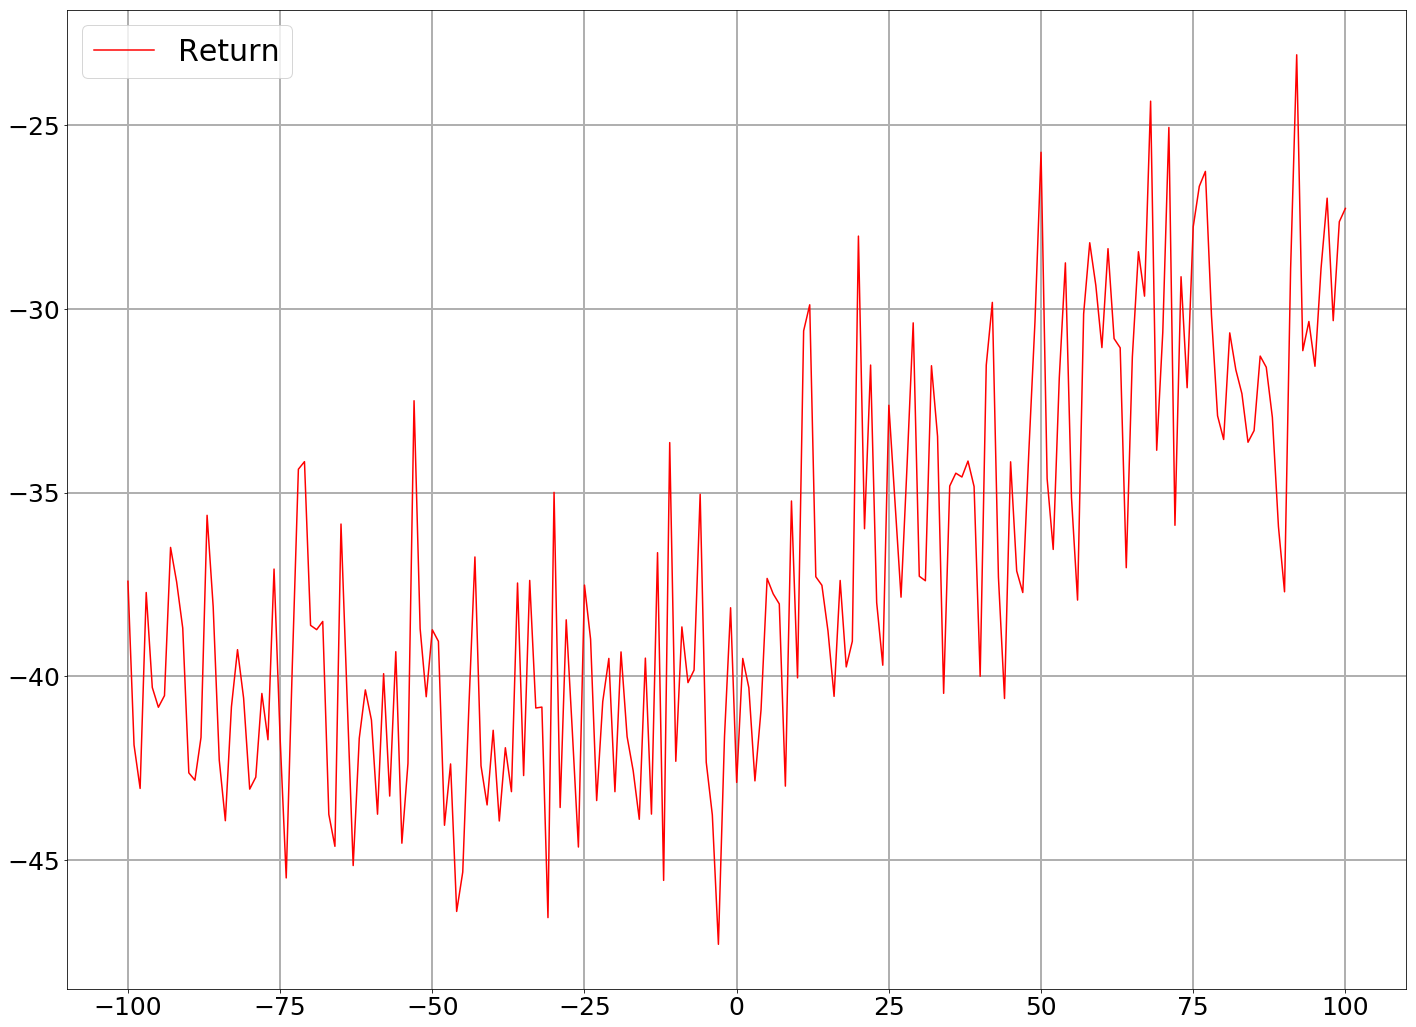
\includegraphics[width=\textwidth]{images/behaviour-100s-sell.png}
        \caption{Returns of sell orders 100 seconds}
        \label{fig:behvaiour-down-100s-sell}
    \end{subfigure}
    \caption{Returns of buy and sell orders executed within 10, 30, 60 and 100 seconds on data set I.}
    \label{fig:behvaiour-down}
\end{figure}

\begin{figure}[H]
    \centering
    \begin{subfigure}[b]{0.45\textwidth}
        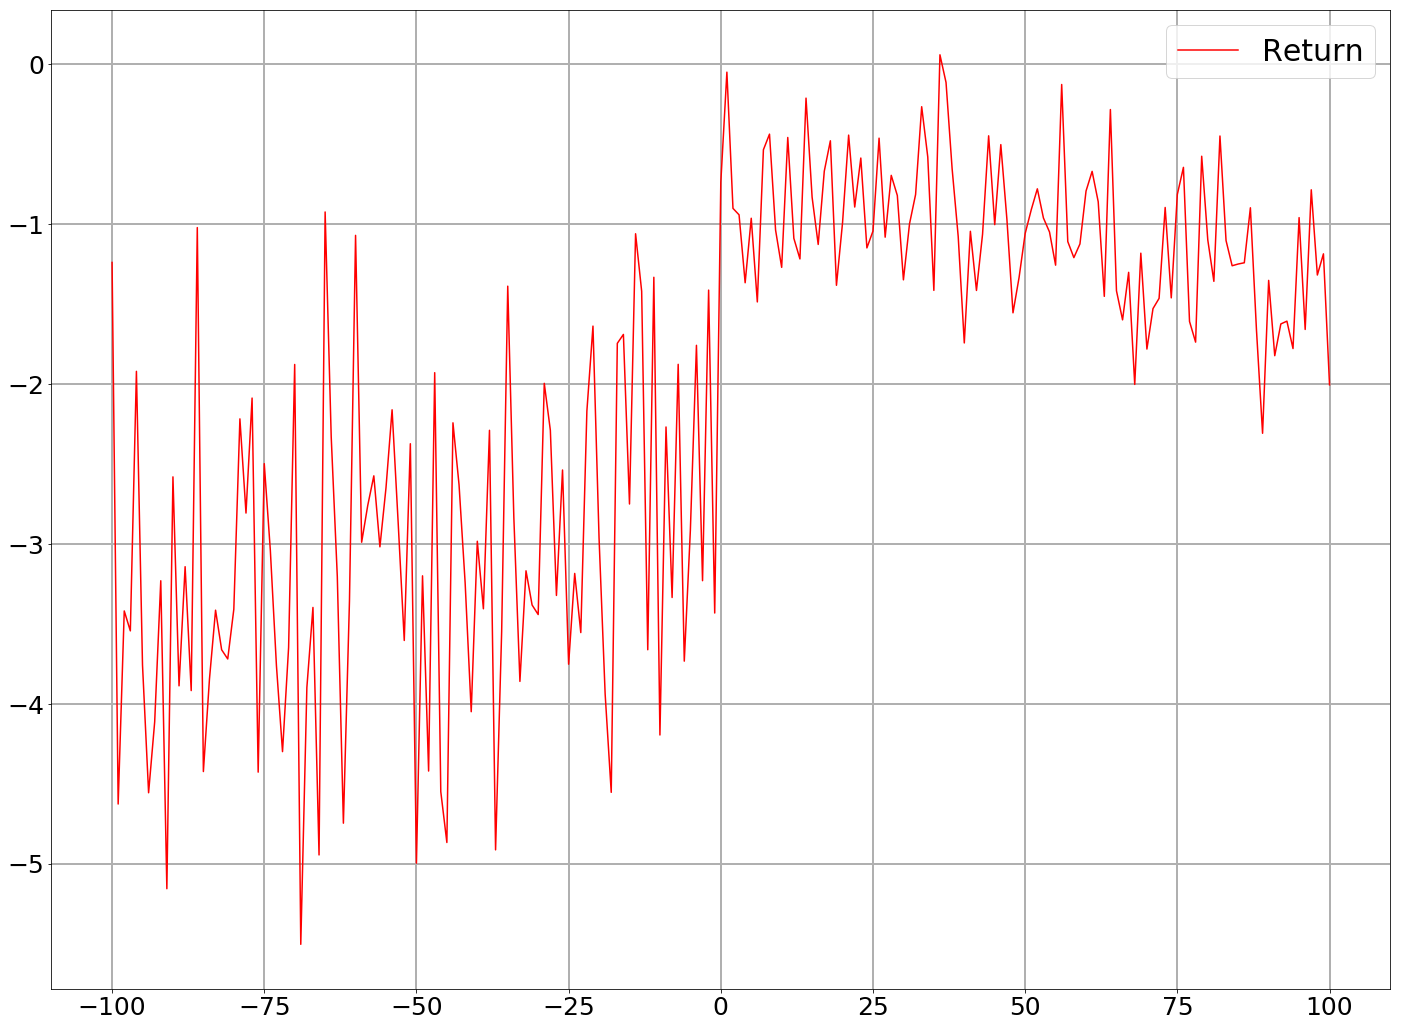
\includegraphics[width=\textwidth]{images/behaviour-up-10s-buy.png}
        \caption{Returns of buy orders within 10 seconds}
        \label{fig:behvaiour-up-10s-buy}
    \end{subfigure}
    \begin{subfigure}[b]{0.45\textwidth}
        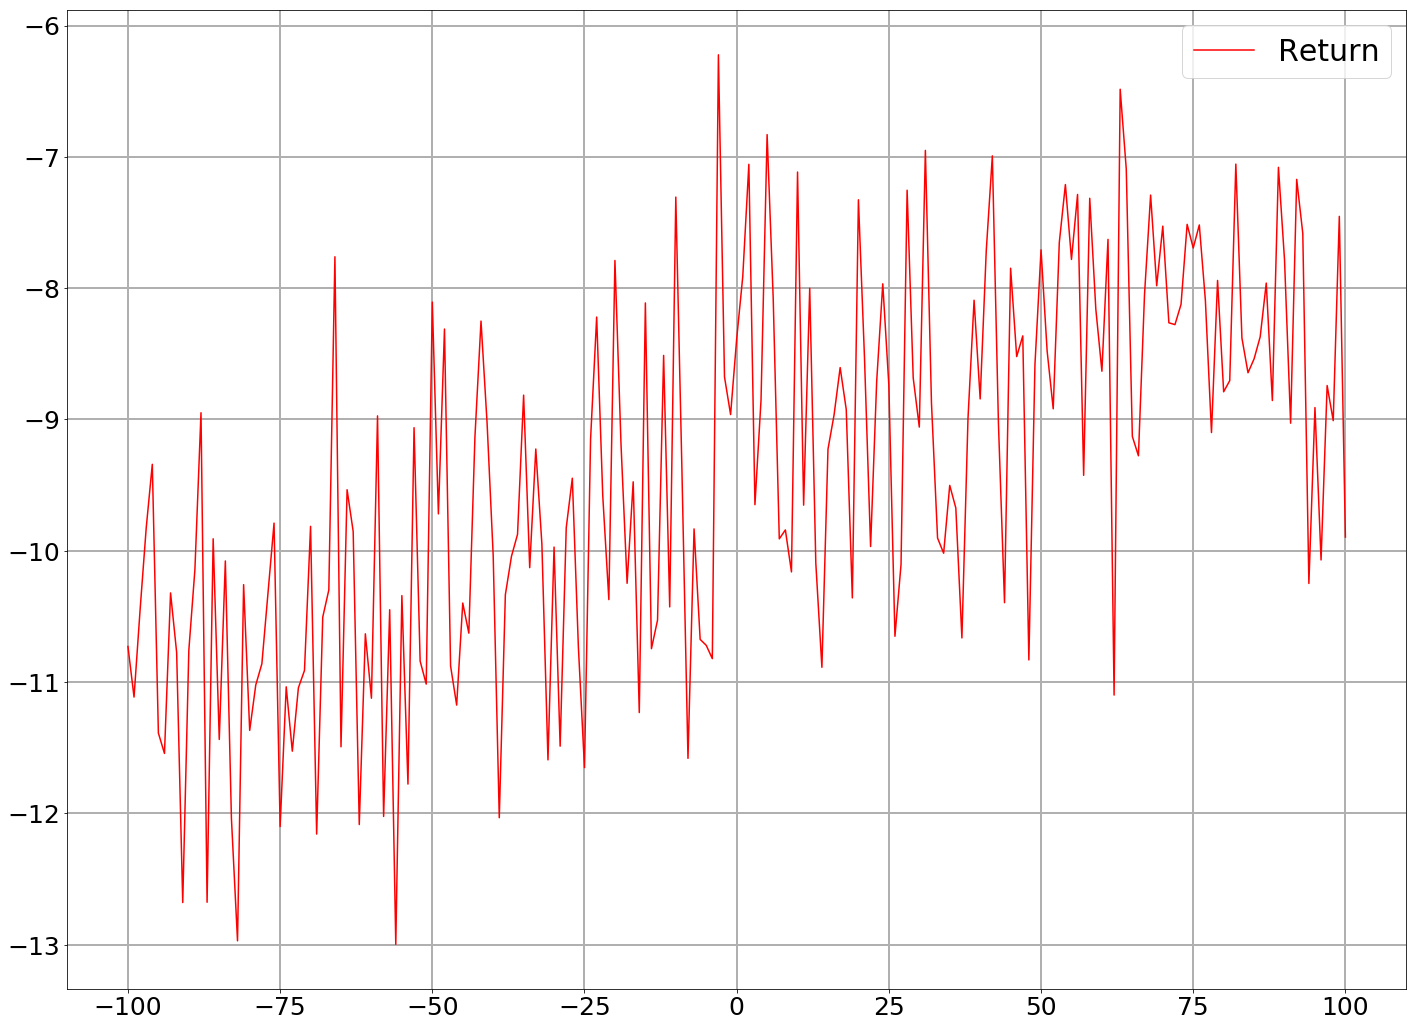
\includegraphics[width=\textwidth]{images/behaviour-up-10s-sell.png}
        \caption{Returns of sell orders within 10 seconds}
        \label{fig:behvaiour-up-10s-sell}
    \end{subfigure}
    \begin{subfigure}[b]{0.45\textwidth}
        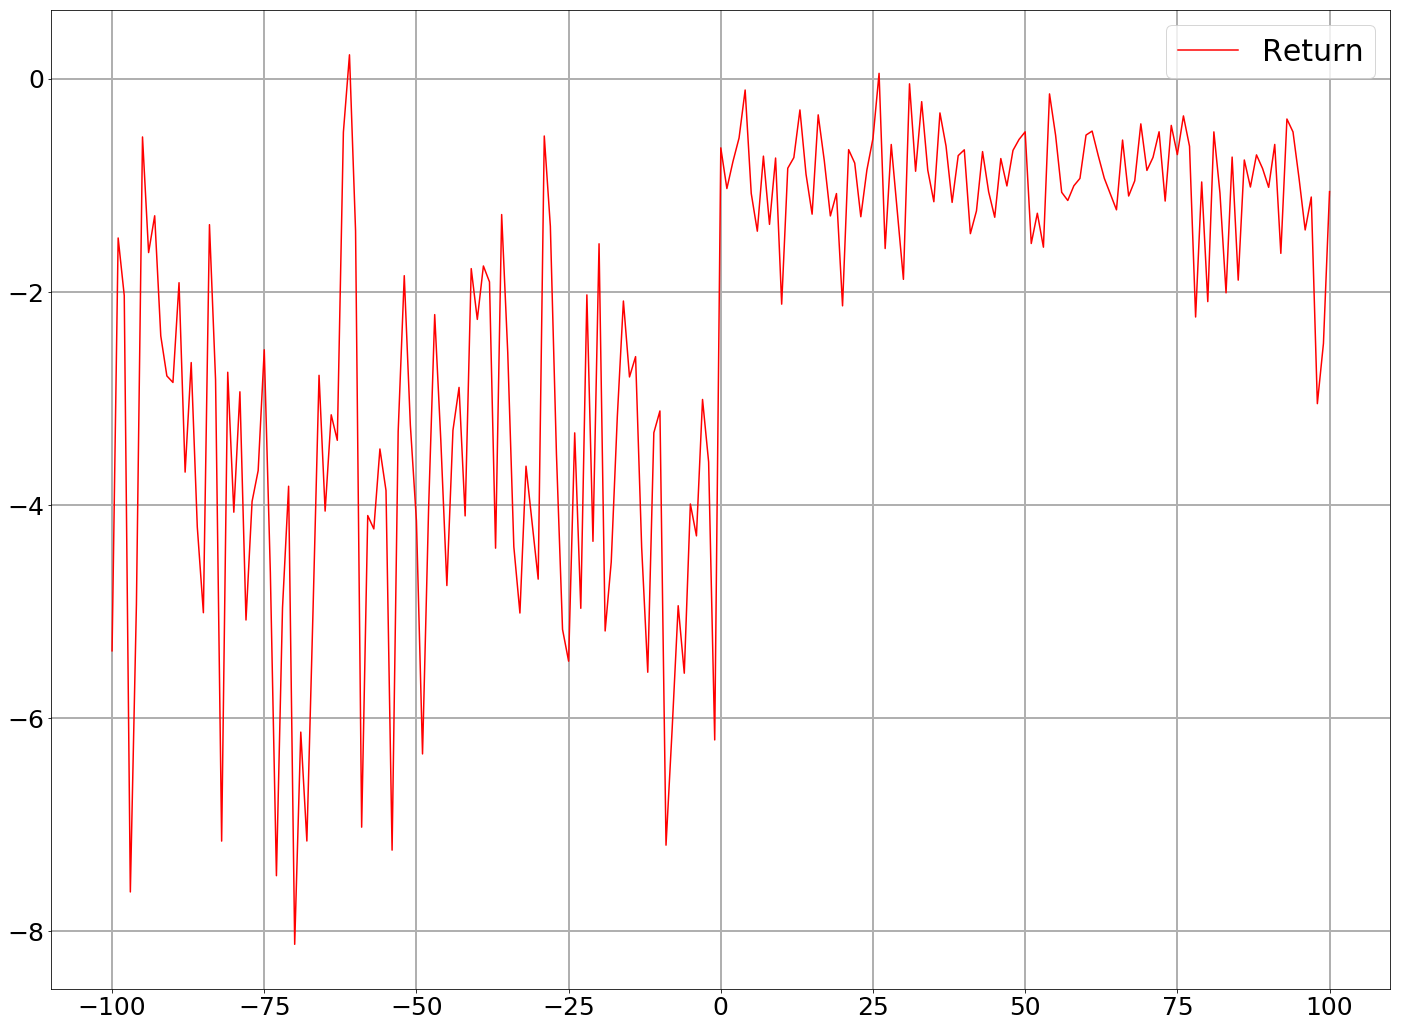
\includegraphics[width=\textwidth]{images/behaviour-up-30s-buy.png}
        \caption{Returns of buy orders within 30 seconds}
        \label{fig:behvaiour-up-30s-buy}
    \end{subfigure}
    \begin{subfigure}[b]{0.45\textwidth}
        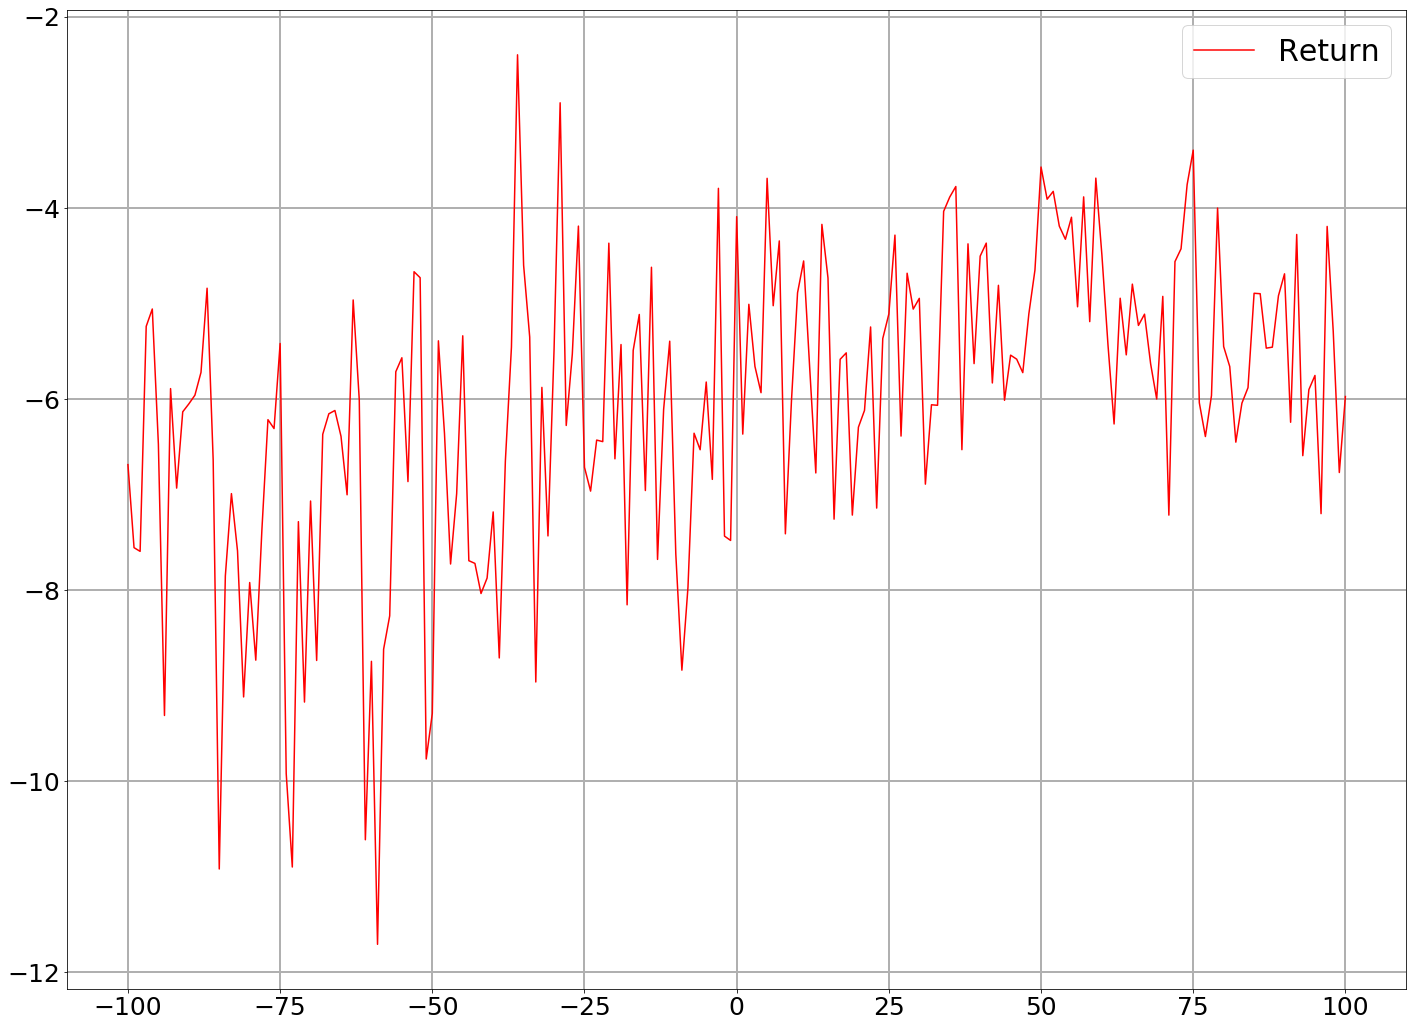
\includegraphics[width=\textwidth]{images/behaviour-up-30s-sell.png}
        \caption{Returns of sell orders within 30 seconds}
        \label{fig:behvaiour-up-30s-sell}
    \end{subfigure}
    \begin{subfigure}[b]{0.45\textwidth}
        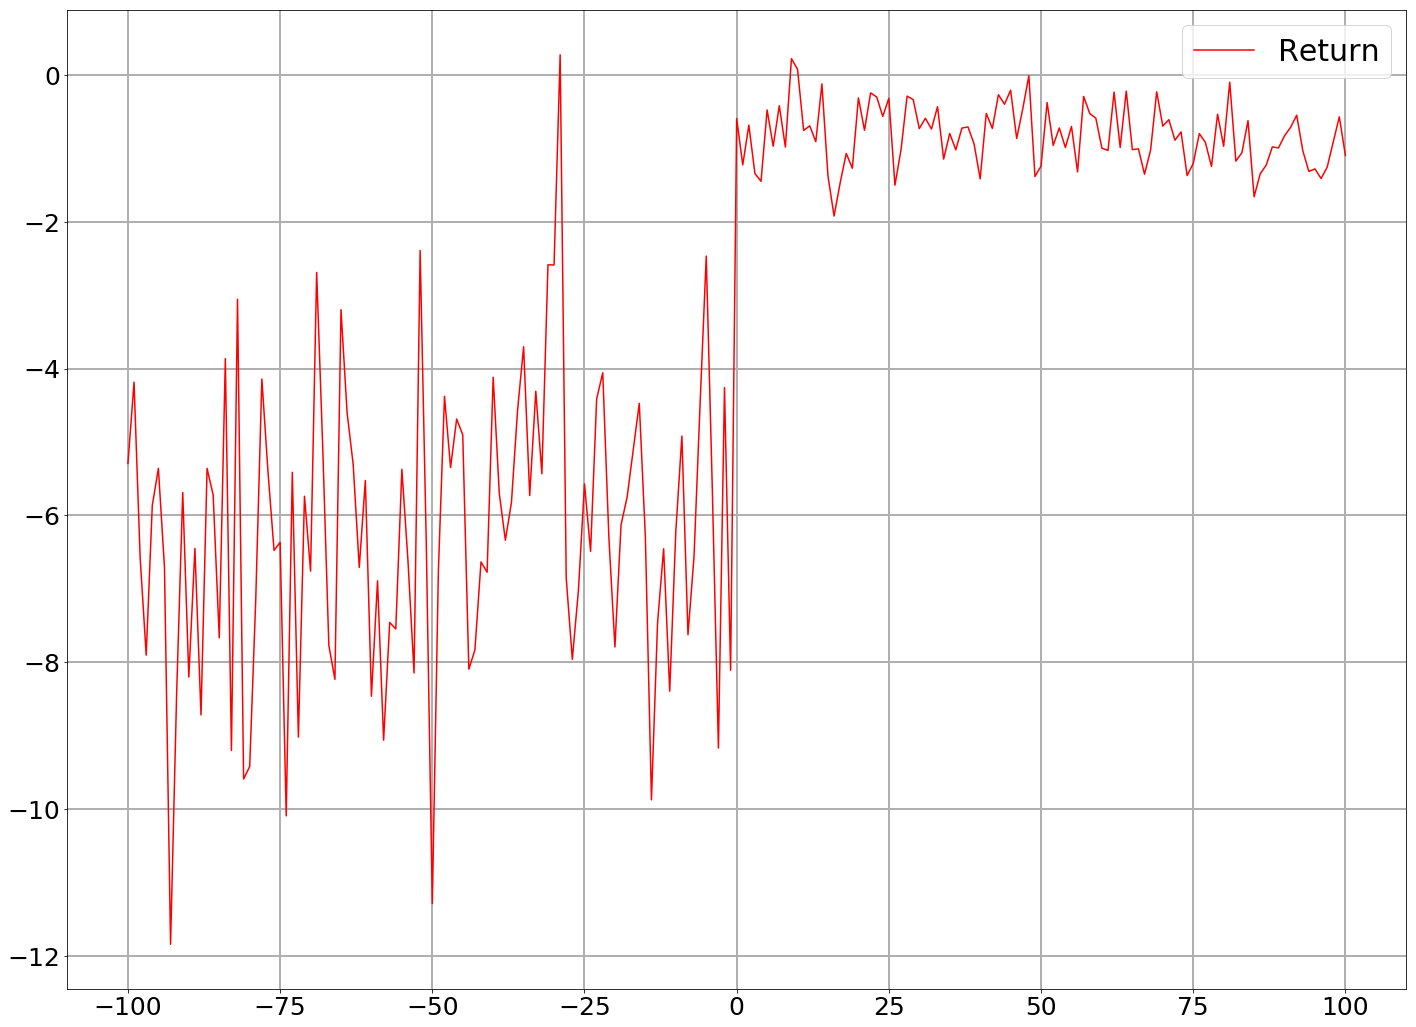
\includegraphics[width=\textwidth]{images/behaviour-up-60s-buy.png}
        \caption{Returns of buy orders within 60 seconds}
        \label{fig:behvaiour-up-60s-buy}
    \end{subfigure}
    \begin{subfigure}[b]{0.45\textwidth}
        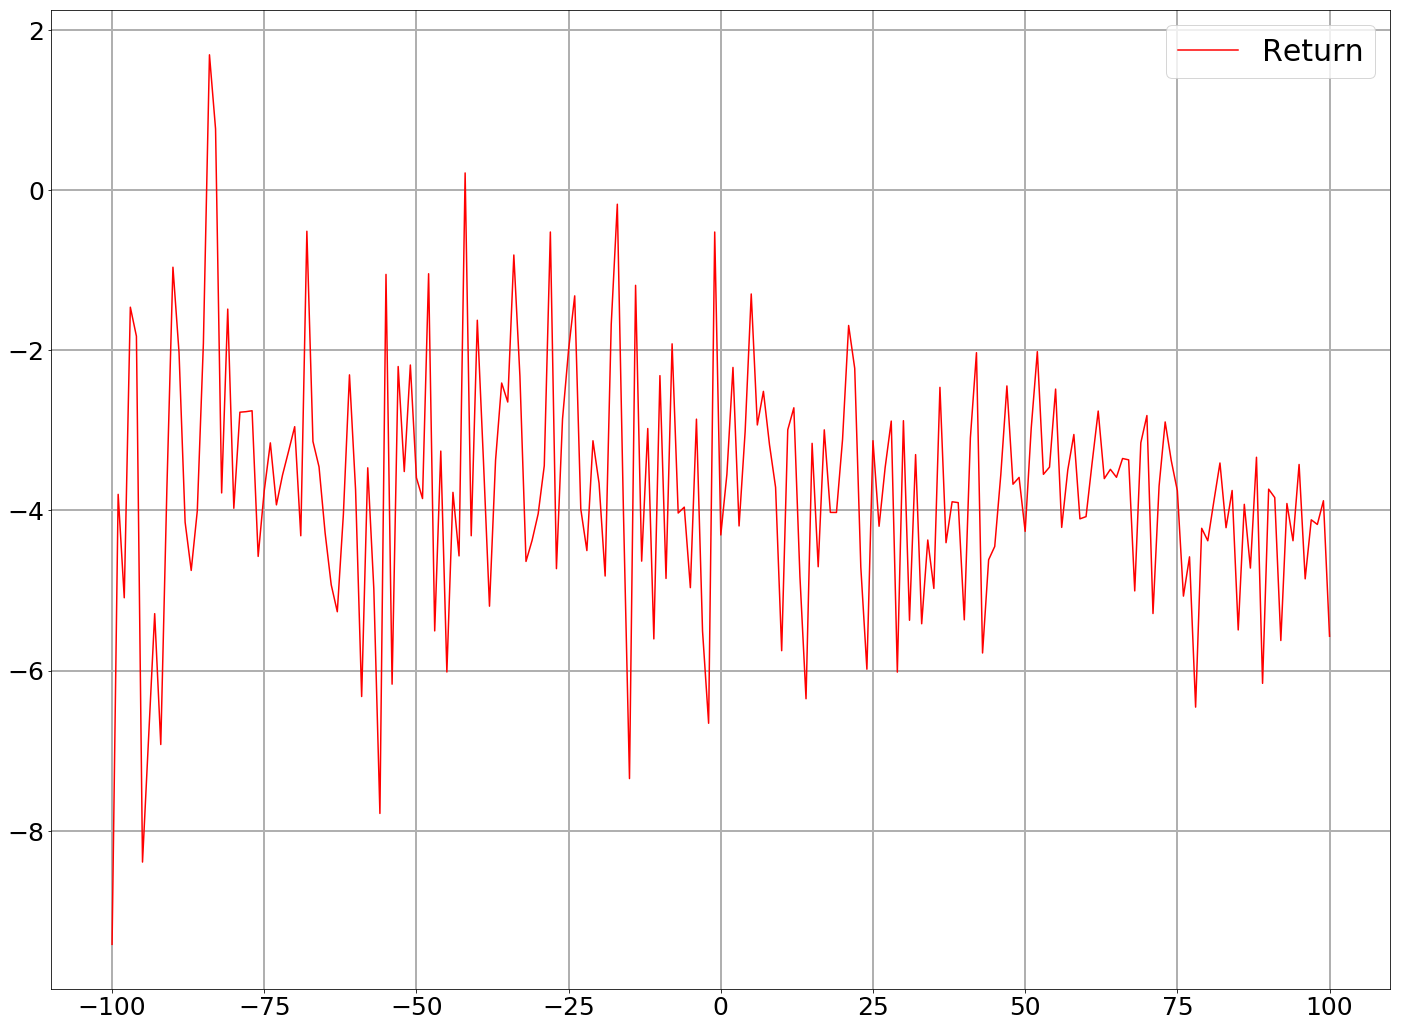
\includegraphics[width=\textwidth]{images/behaviour-up-60s-sell.png}
        \caption{Returns of sell orders 60 seconds}
        \label{fig:behvaiour-up-60s-sell}
    \end{subfigure}
    \begin{subfigure}[b]{0.45\textwidth}
        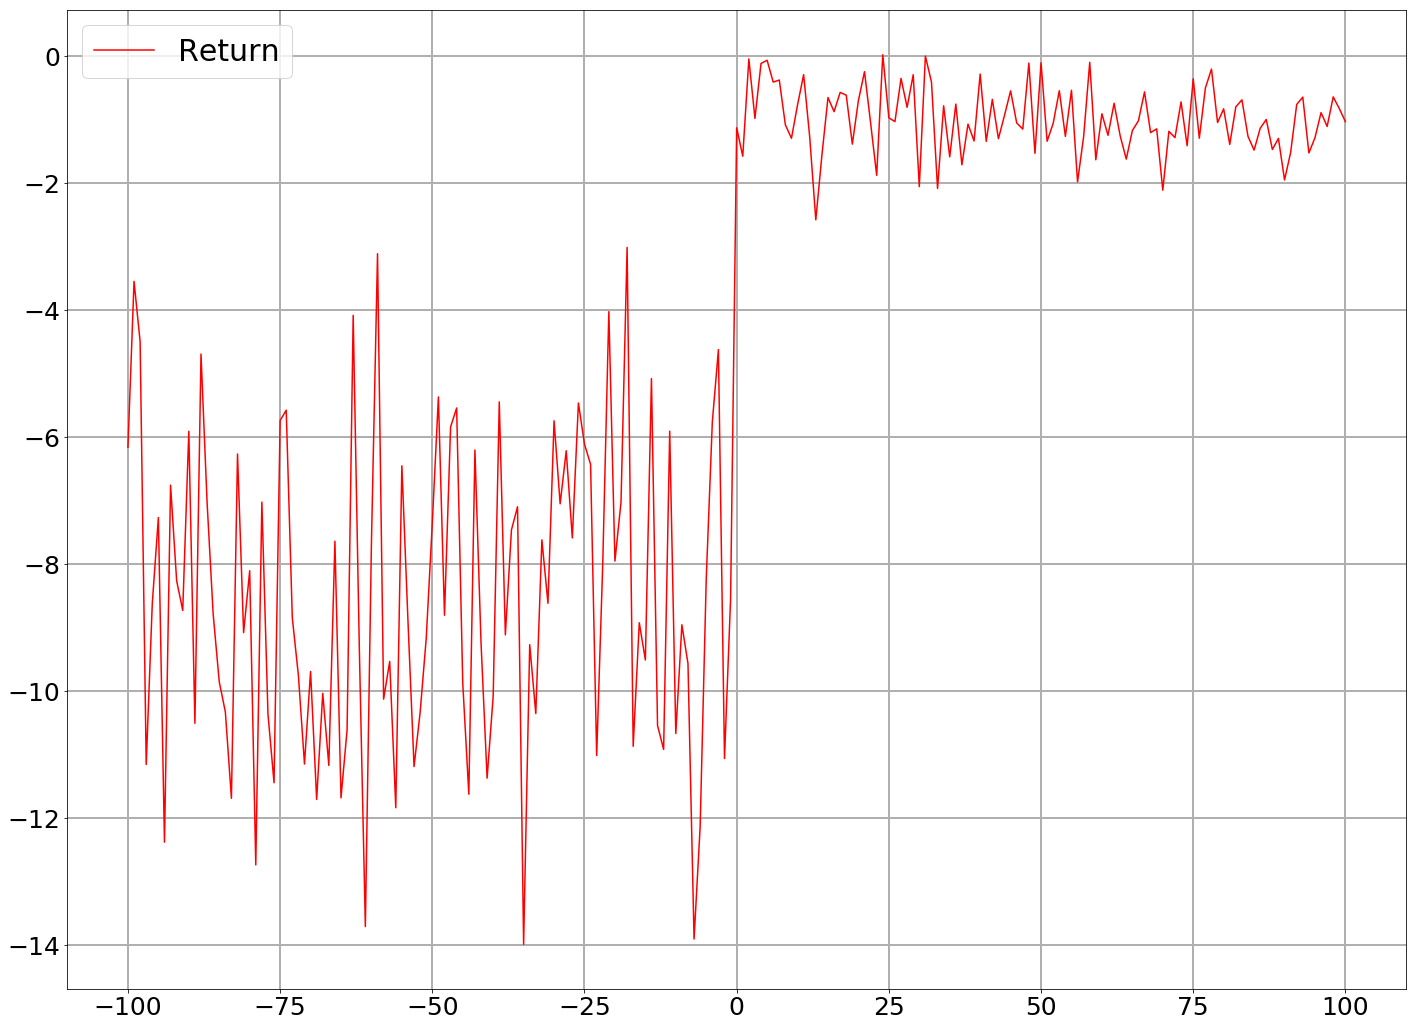
\includegraphics[width=\textwidth]{images/behaviour-up-100s-buy.png}
        \caption{Returns of buy orders 100 seconds}
        \label{fig:behvaiour-up-100s-buy}
    \end{subfigure}
    \begin{subfigure}[b]{0.45\textwidth}
        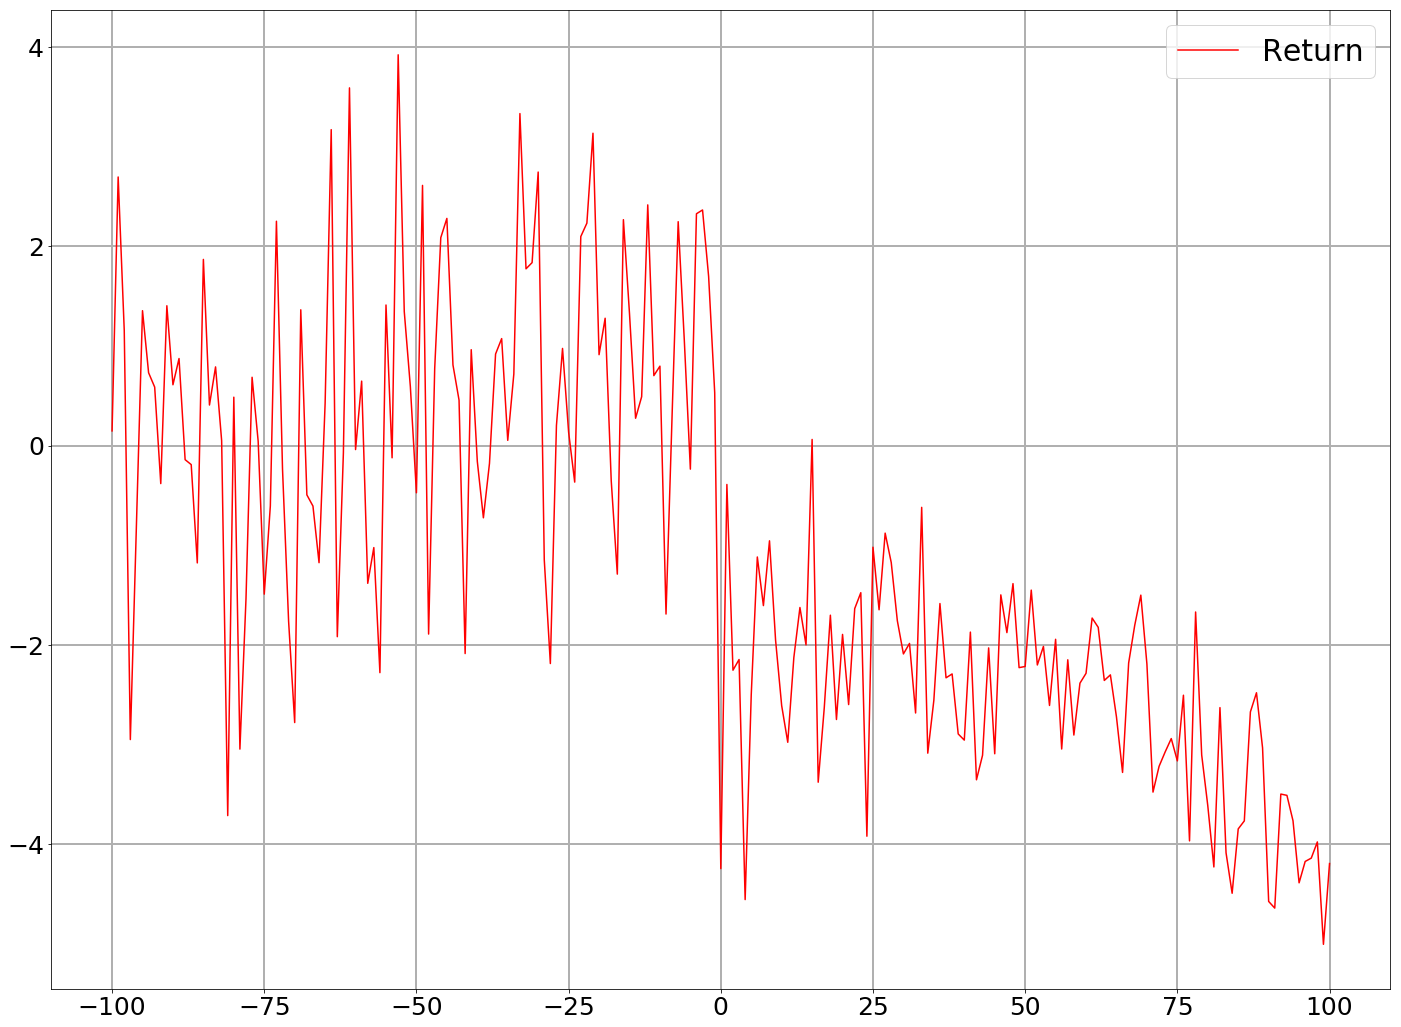
\includegraphics[width=\textwidth]{images/behaviour-up-100s-sell.png}
        \caption{Returns of sell orders 100 seconds}
        \label{fig:behvaiour-up-100s-sell}
    \end{subfigure}
    \caption{Returns of buy and sell orders executed within 10, 30, 60 and 100 seconds on data set II.}
    \label{fig:behvaiour-up}
\end{figure}

\subsection{Order placement behavior on data set II}
For data set II, which shows an upward price trend, the assumption is the opposite as stated for the investigation using data set I.
We expect buy orders to result in better returns when immediately filled, that is, when the agent crosses the spread and places the order high in the book ($a>0$).
The assumption is that, as time passes and the market price rises, other traders become less willing to sell at the market price or lower.
Therefore, the longer the time horizon given to the agent, the more critical it becomes to execute immediately;  otherwise, shares would have to be bought at an increased market price.
In contrast, better returns with sell orders are expected when placed deep in the book ($a<0$), meaning that they are sold at a higher price.
The assumption is that, as the price rises, market participants become more likely to buy assets at higher prices.
Hence, the longer the time horizon, the deeper in the book the agent should place a limit sell order.
We investigated these assumptions by performing the same experiment as in the previous section, with time horizons of 10, 30, 60 and 100 seconds, as shown in Figure \ref{fig:behvaiour-up}.

The returns of buy orders filled within a time horizon of 10 seconds, as shown in Figure \ref{fig:behvaiour-up-10s-buy}, correlate with the above-mentioned assumptions.
The highest returns are achieved when crossing the spread and, although limit levels in the range of 1-50 tend to perform the same, and considering the risk of paying a premium, the wisest choice for the agent would be to choose the level closest to the spread.
The sell orders placed with a time horizon of 10 seconds contradict the assumptions, as shown in Figure \ref{fig:behvaiour-up-10s-sell}.
The agent obtains the highest rewards when choosing a price for the order at market price $a=0$.
A highly negative limit level yields a return of  approximately \$3.00 less than when placing at the suggested market price.

With 30 seconds left to buy 1.0 BTC (Figure \ref{fig:behvaiour-up-30s-buy}), the orders placed with $a>0$ (above the spread) become stable for any such limit level.
This is likely due to the higher order pressure of data set II, as described in Section \ref{sec:analysis-data-sets}, as there are more market participants willing to sell.
The returns for limit sell orders, as shown in Figure \ref{fig:behvaiour-up-30s-sell}, became more rewarding as the agent benefits from a slight increase in price within the given time horizon.

This pattern becomes clearly apparent when a time horizon of 60 and 100 seconds was given, as shown in Figures \ref{fig:behvaiour-up-60s-sell} and \ref{fig:behvaiour-up-100s-sell} respectively.
With this increased time horizon, the assumptions stated in the beginning of this section are confirmed and the agent, when trying to sell shares, should indeed place orders deep in the order book ($a<0$).
As time passes and the market price rises, market participants are willing to buy at an increased price and the agent is expected to be able to sell all assets at this increased price without the need for a further market order.
In contrast, if the agent decides to sell the assets at decreasing prices, as indicated by the higher limit levels (when $a>0$), a lower reward can be expected.
More precisely, for a time horizon of 100 seconds, the agent is expected to receive up to \$7.00 less when choosing to cross the spread with an action of +100, as opposed to a negative action.
Figures \ref{fig:behvaiour-up-60s-buy} and \ref{fig:behvaiour-up-100s-buy} show the expected results of an agent that buys assets within 60 and 100 seconds respectively.
It is evident from the figures that the rise in the market price means that the expected damage can be minimized by crossing the spread and buying immediately.
The proposition stated before remains valid: the agent should choose a price slightly above the market price as there is enough liquidity in the market to buy the demanded number of assets.

\subsection{Conclusion of empirical analysis}
From the results of the empirical analysis performed on data sets I and II, the following observations can be made with respect to limit order placement:
during a fall in the market price, the purchase prices of assets can be optimized by placing limit orders deep in the order book ($a<0$) and the least loss is sustained when selling assets immediately at the market price ($a>0$).
In contrast, during a rising market, it is suggested that assets be purchased using a market order ($a>0$) and sale prices can be optimized by placing the sell orders deep in the order book ($a<0$).
These effects become more apparent when a longer time horizon is given for an order. With regard to shorter time horizons, the order placement process tends to be either intercepted by short term fluctuations or low trading volumes.
The latter implies that, during an upwards trend, market participants are willing to buy and sell shares at higher prices and on the contrary, during a downwards trend at lower prices.
In this experiment, the orders placed had to be completely filled without the ability to take intermediate steps of canceling and replacing the order within the given time horizon.
Therefore, it falls to the reinforcement learners to evaluate whether or not such amendments to the order will result in a more favorable reward.
In order to have a measure of comparison for the reinforcement learning agents to come, Table \ref{tbl:analysis-empirical-summary} summarizes the findings and shows the expected rewards for (1) the optimal limit level chosen and (2) an immediate completion of the order using a market order.
\begin{table}[H]
\centering
\begin{tabular}{l|l|l|}
\cline{2-3}
& \textbf{$\mathbb{E}$[Limit order] (optimal)} & \textbf{\begin{tabular}[c]{@{}l@{}}$\mathbb{E}$[Market order]\end{tabular}} \\ \hline
\multicolumn{1}{|l|}{\textbf{Buy (I)}}   & 15.20          & -0.05                                                           \\ \hline
\multicolumn{1}{|l|}{\textbf{Sell (I)}}  & -27.70         & -27.70                                                          \\ \hline
\multicolumn{1}{|l|}{\textbf{Buy (II)}}  & -1.06          & -1.06                                                           \\ \hline
\multicolumn{1}{|l|}{\textbf{Sell (II)}} & 3.68          & -1.72                                                           \\ \hline
\multicolumn{1}{|l|}{\textbf{$\Sigma$}} & -9.88          & -30.53                                                           \\ \hline
\end{tabular}
\caption{Summary of rewards derived from the empirical analysis.}
\label{tbl:analysis-empirical-summary}
\end{table}

Furthermore, we ran the same experiment by using different action step parameters $\Delta{a}$, as shown in Table \ref{tbl:analysis-empirical-summary-a}.
Thereby, we found that a coarser step size does not improve the expected return for an optimal placed limit order.
As a result, we will henceforth use the setting $\Delta{a}=\$0.1$ for investigations undertaken with reinforcement learning agents.
\begin{table}[H]
\centering
\begin{tabular}{l|l|l|l|l|}
\cline{2-5} & \textbf{$\Delta{a}=\$0.1$} & \textbf{$\Delta{a}=\$0.2$} & \textbf{$\Delta{a}=\$0.5$} & \textbf{$\Delta{a}=\$1.0$} \\ \hline
\multicolumn{1}{|l|}{\textbf{\begin{tabular}[c]{@{}l@{}}$\mathbb{E}${[}Limit order{]} \\ (optimal)\end{tabular}}} & -9.88          & -9.96          & -13.52         & -17.65         \\ \hline
\end{tabular}
\caption{Rewards derived from the empirical analysis with different action step parameters $\Delta{a}$.}
\label{tbl:analysis-empirical-summary-a}
\end{table}

\section{Q-Learning without market variables}
\label{sec:eval-qlearn}
The previous section provided the expected rewards an agent receives when placing buy and sell orders using the reinforcement learning environment under the application of data set I and II.
For each observation, a fixed time horizon was chosen for which an orders were placed in the order book, followed by a market orders in case the orders were not filled completely.

This section aims to investigate whether or not a Q-Learning agent, as described in Chapter \ref{chap:setup} (Section \ref{setup:q-learning}), can improve with respect to the rewards received.
Thereby, the agent is allowed to cancel its order after every 10 seconds (e.g. $\Delta{t}=10$) and place a new order on the basis of the remaining inventory, until the time horizon of 100 seconds expires.
Subsequently, and in the event that an order has not been filled completely, a market order is submitted for the remaining share to be bought or sold.
For both data sets (I and II), an independent learning experiment was proceeded where the agent had to either buy or sell shares.
In each experiment, the training was limited to 5000 epochs and 1000 orders were placed and evaluated on the test set (defined as "backtesting").
The Q-Learning agent was set up as follows:
the learning rate selected $\alpha=0.1$ is small due to the extensive number of steps the agent will take throughout the epochs.
The discount factor $\gamma=0.5$ is chosen to balance the agent's incentive to profit from immediate and future rewards.
Initially, the exploration constant $\epsilon$ is set to 0.8 and a decay is applied such that the factor reduces to $\epsilon=0.1$ by the time the training is completed.
This allows the agent first to explore the action space and then exploit on the learned optimal actions to take.

With this setup, four observations were made and for each, the training and testing results are stated below.
During training, the mean rewards and the average action chosen for each epoch were recorded.
Once the model was trained, a backtest was run on the test data sets, in which the agent executed orders by choosing from the learned policy.

\subsection{Results of training and testing on data sets I and II}

\begin{figure}
    \centering
    \begin{subfigure}[b]{0.4\textwidth}
        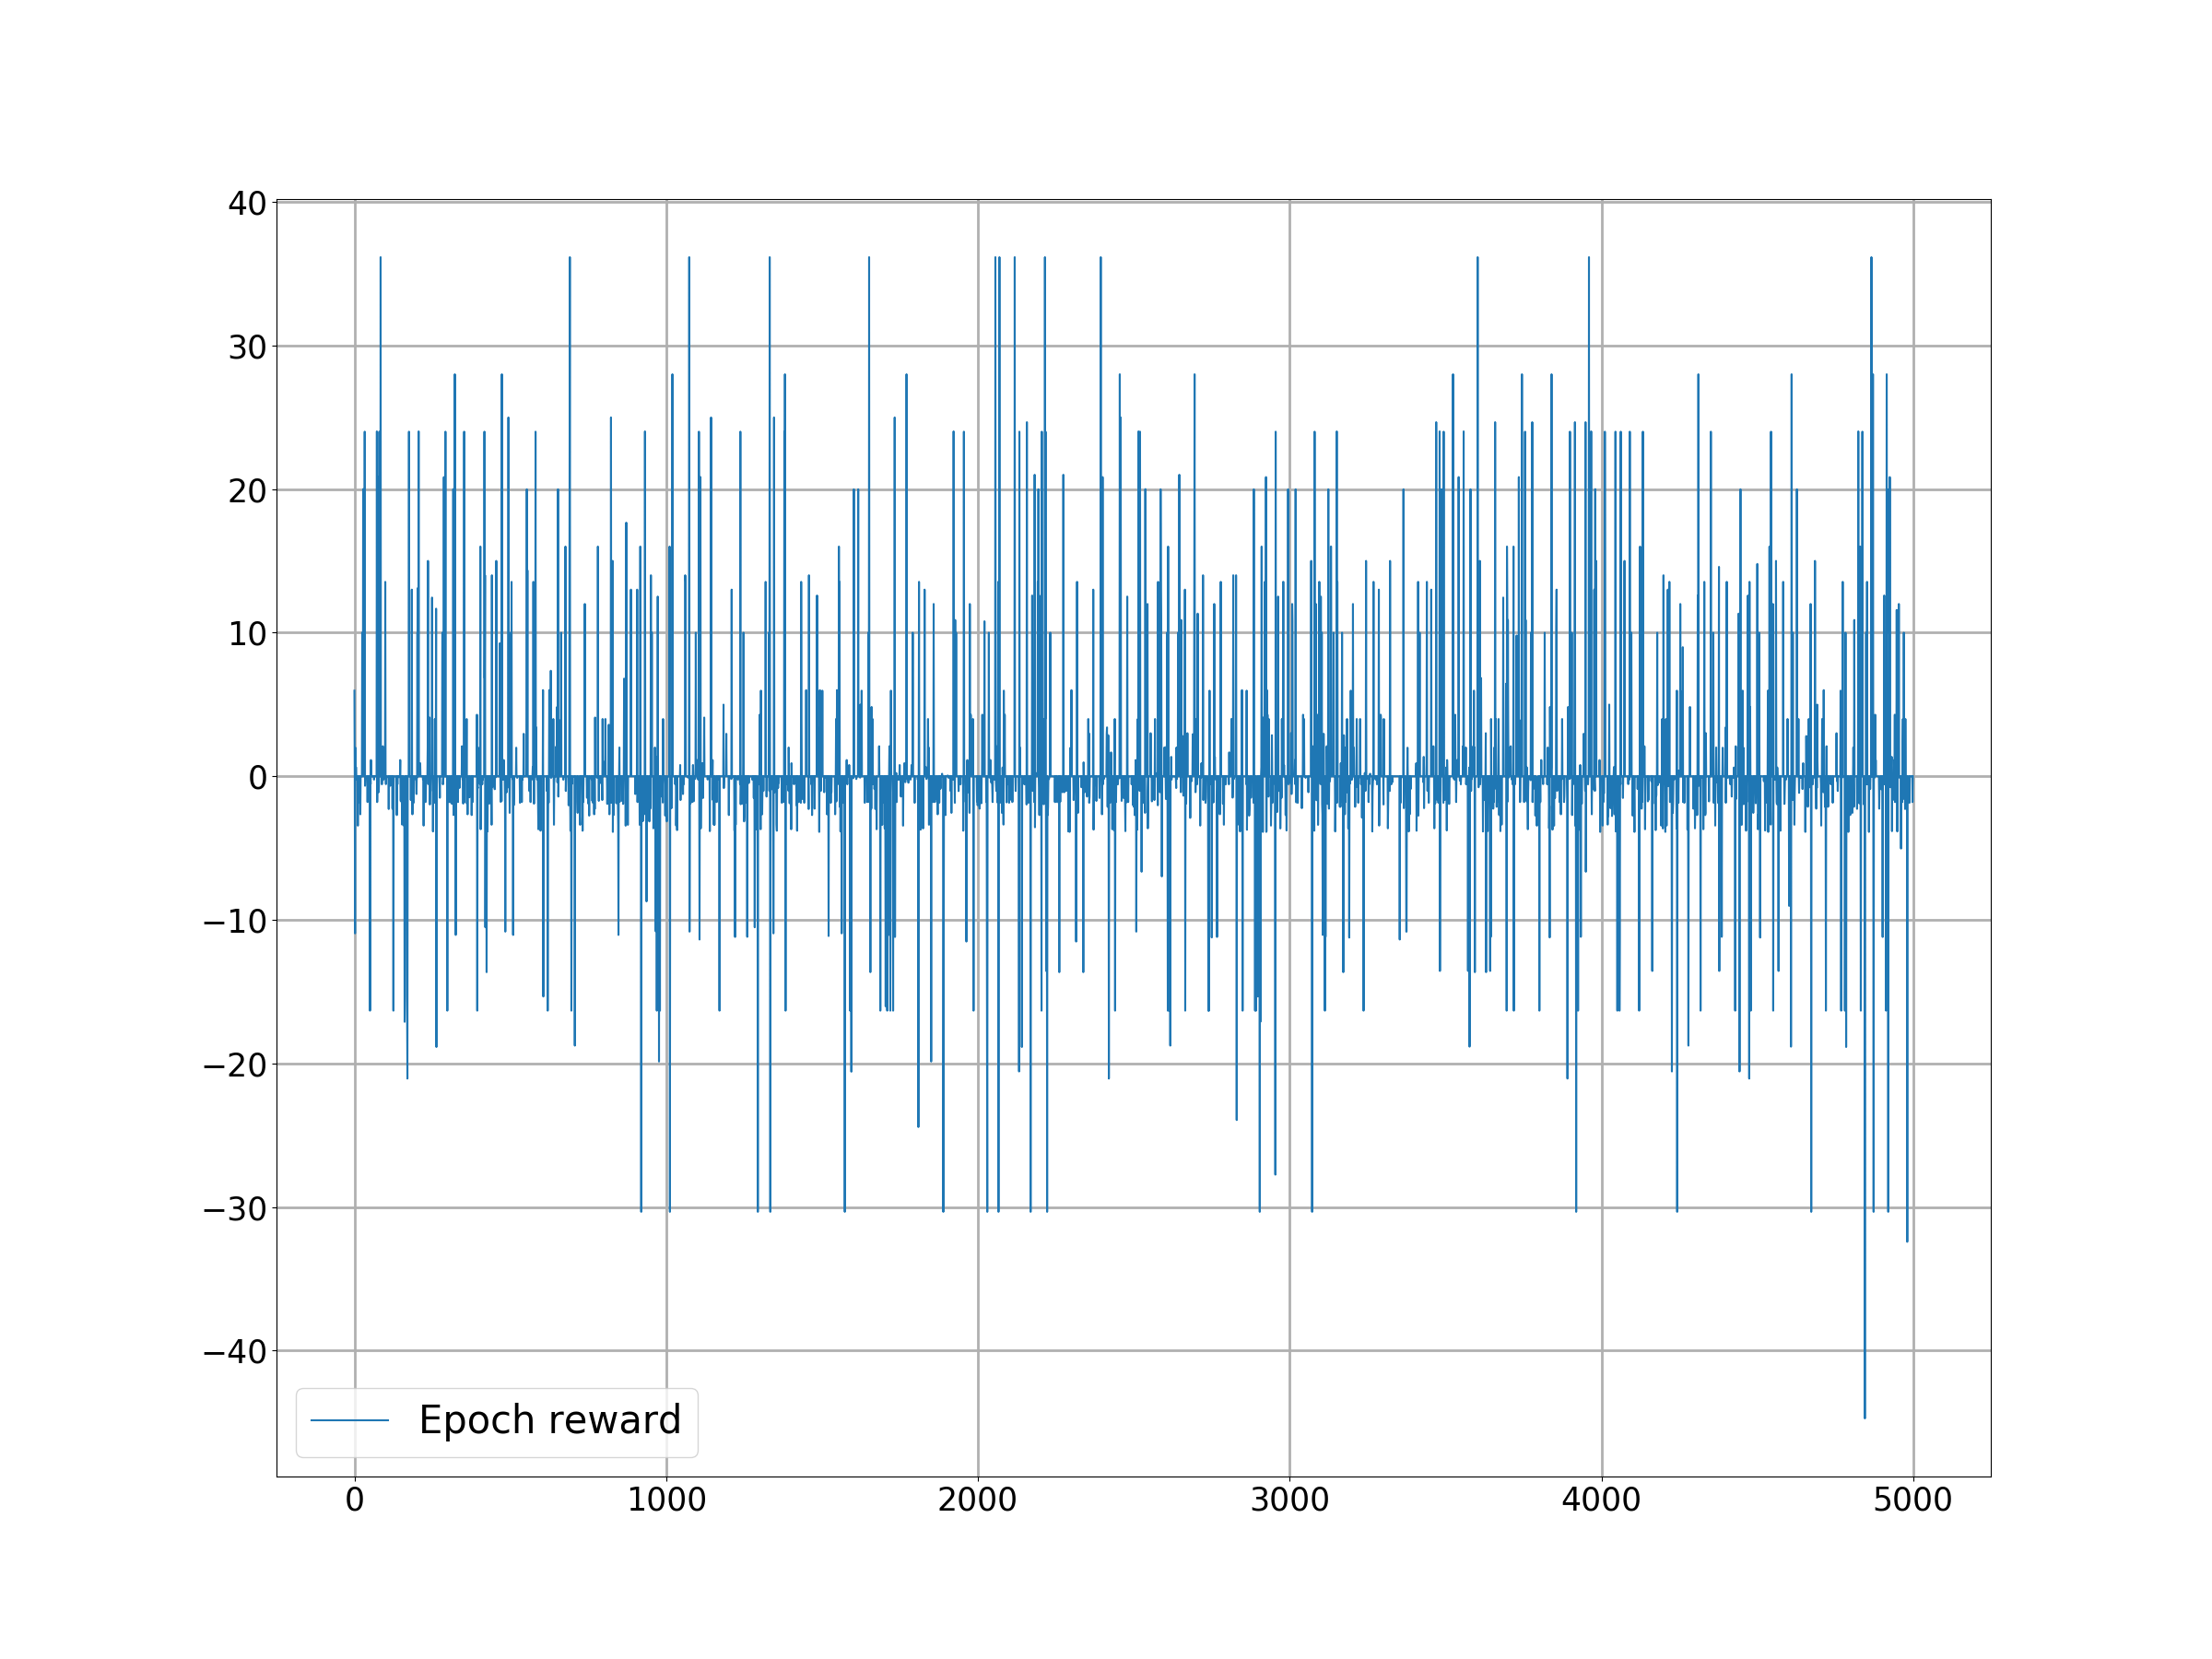
\includegraphics[width=\textwidth]{q_1_10000_BUY_rewards.png}
        \caption{Mean rewards per epoch (buy)}
        \label{fig:analysis-q-learn-1-reward-buy}
    \end{subfigure}
    \begin{subfigure}[b]{0.4\textwidth}
        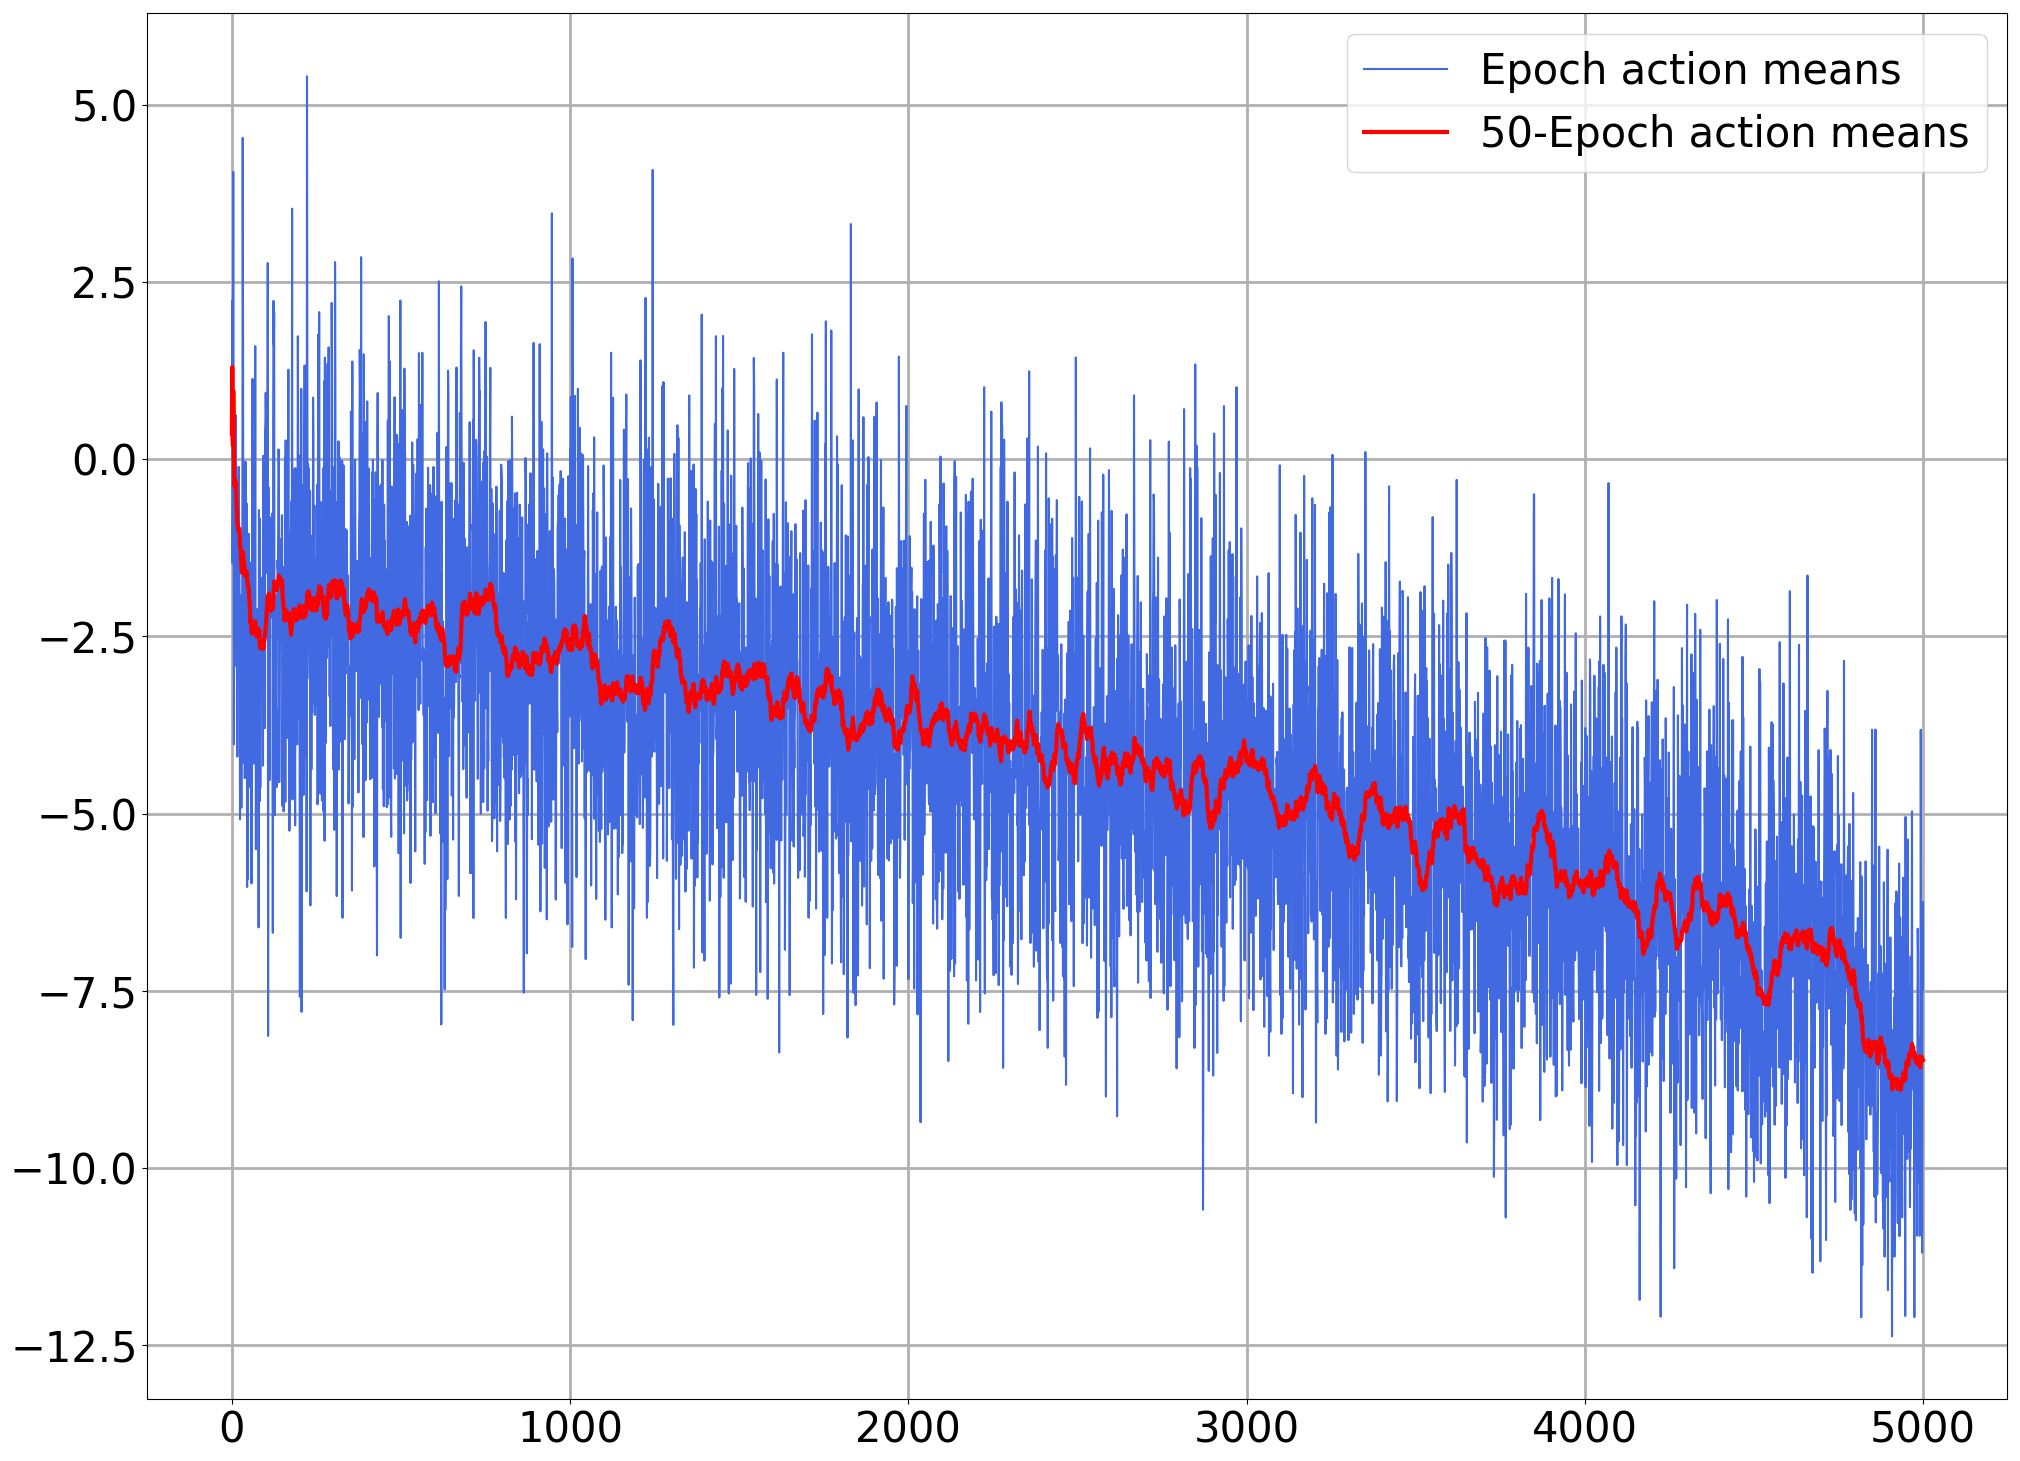
\includegraphics[width=\textwidth]{q_1_10000_BUY_mean_actions.png}
        \caption{Mean of actions per epoch (buy)}
        \label{fig:analysis-q-learn-1-action-buy}
    \end{subfigure}
    \begin{subfigure}[b]{0.4\textwidth}
        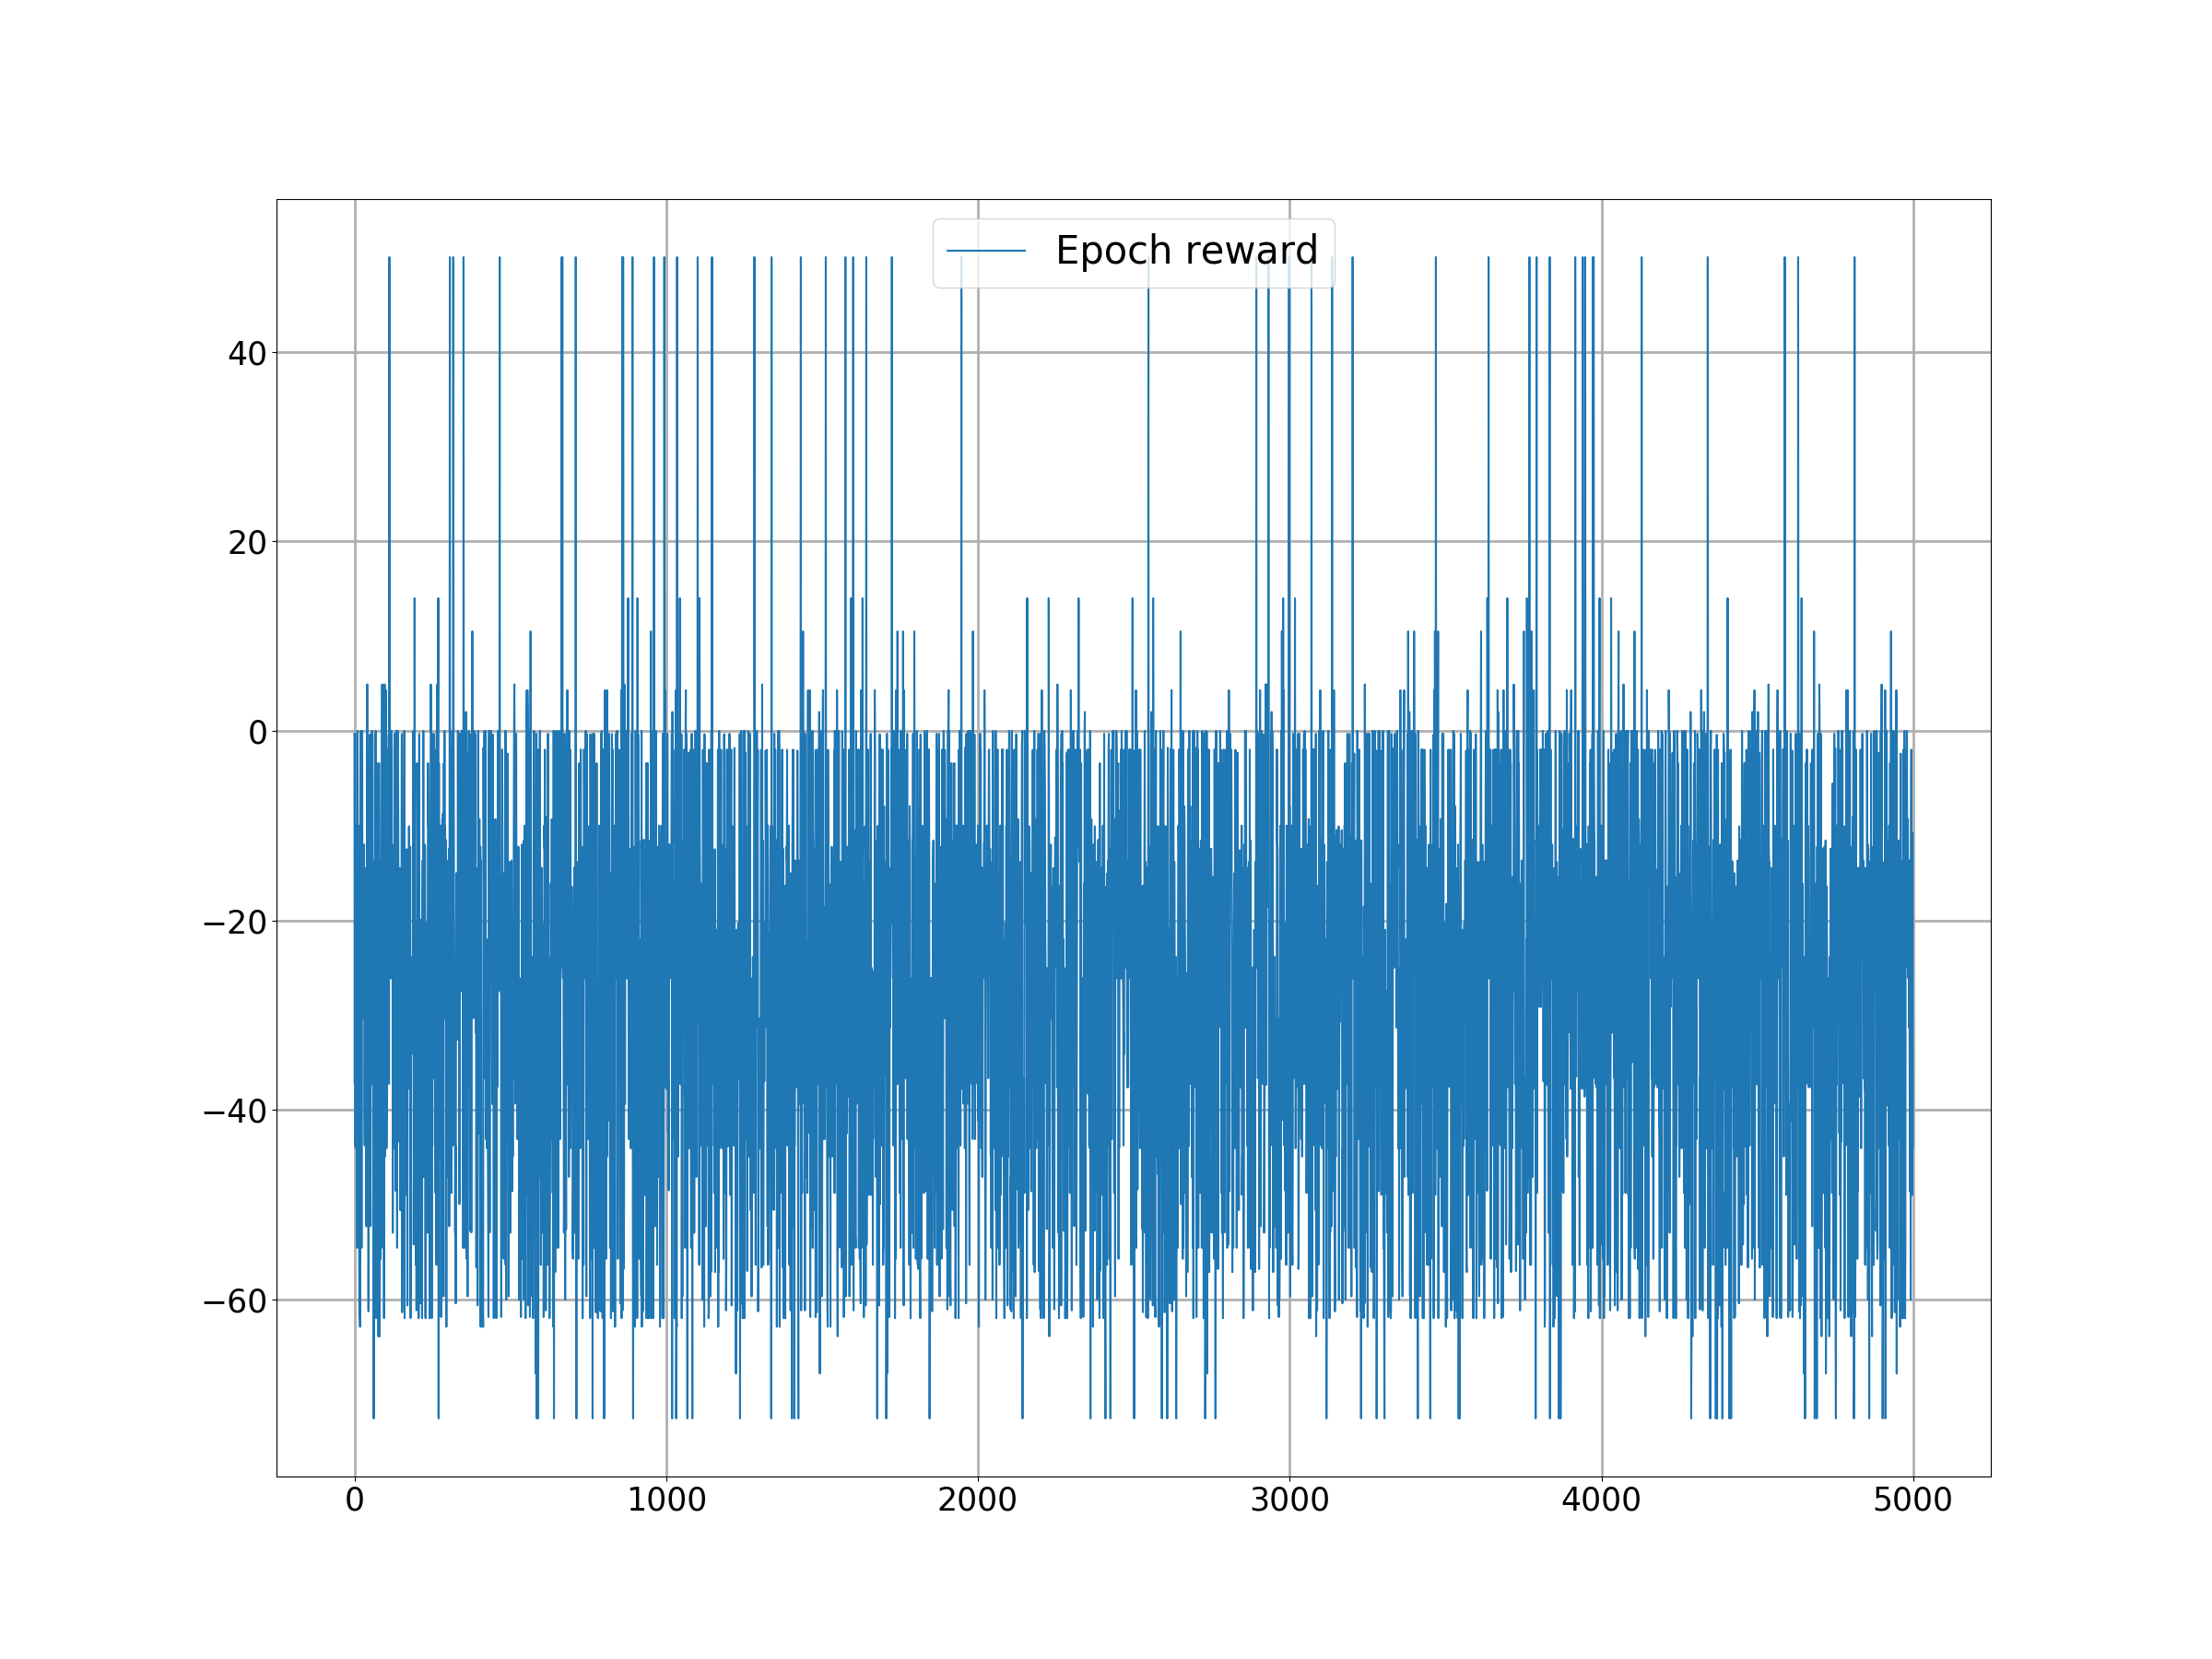
\includegraphics[width=\textwidth]{q_1_10000_SELL_rewards.png}
        \caption{Mean rewards per epoch (sell)}
        \label{fig:analysis-q-learn-1-reward-sell}
    \end{subfigure}
    \begin{subfigure}[b]{0.4\textwidth}
        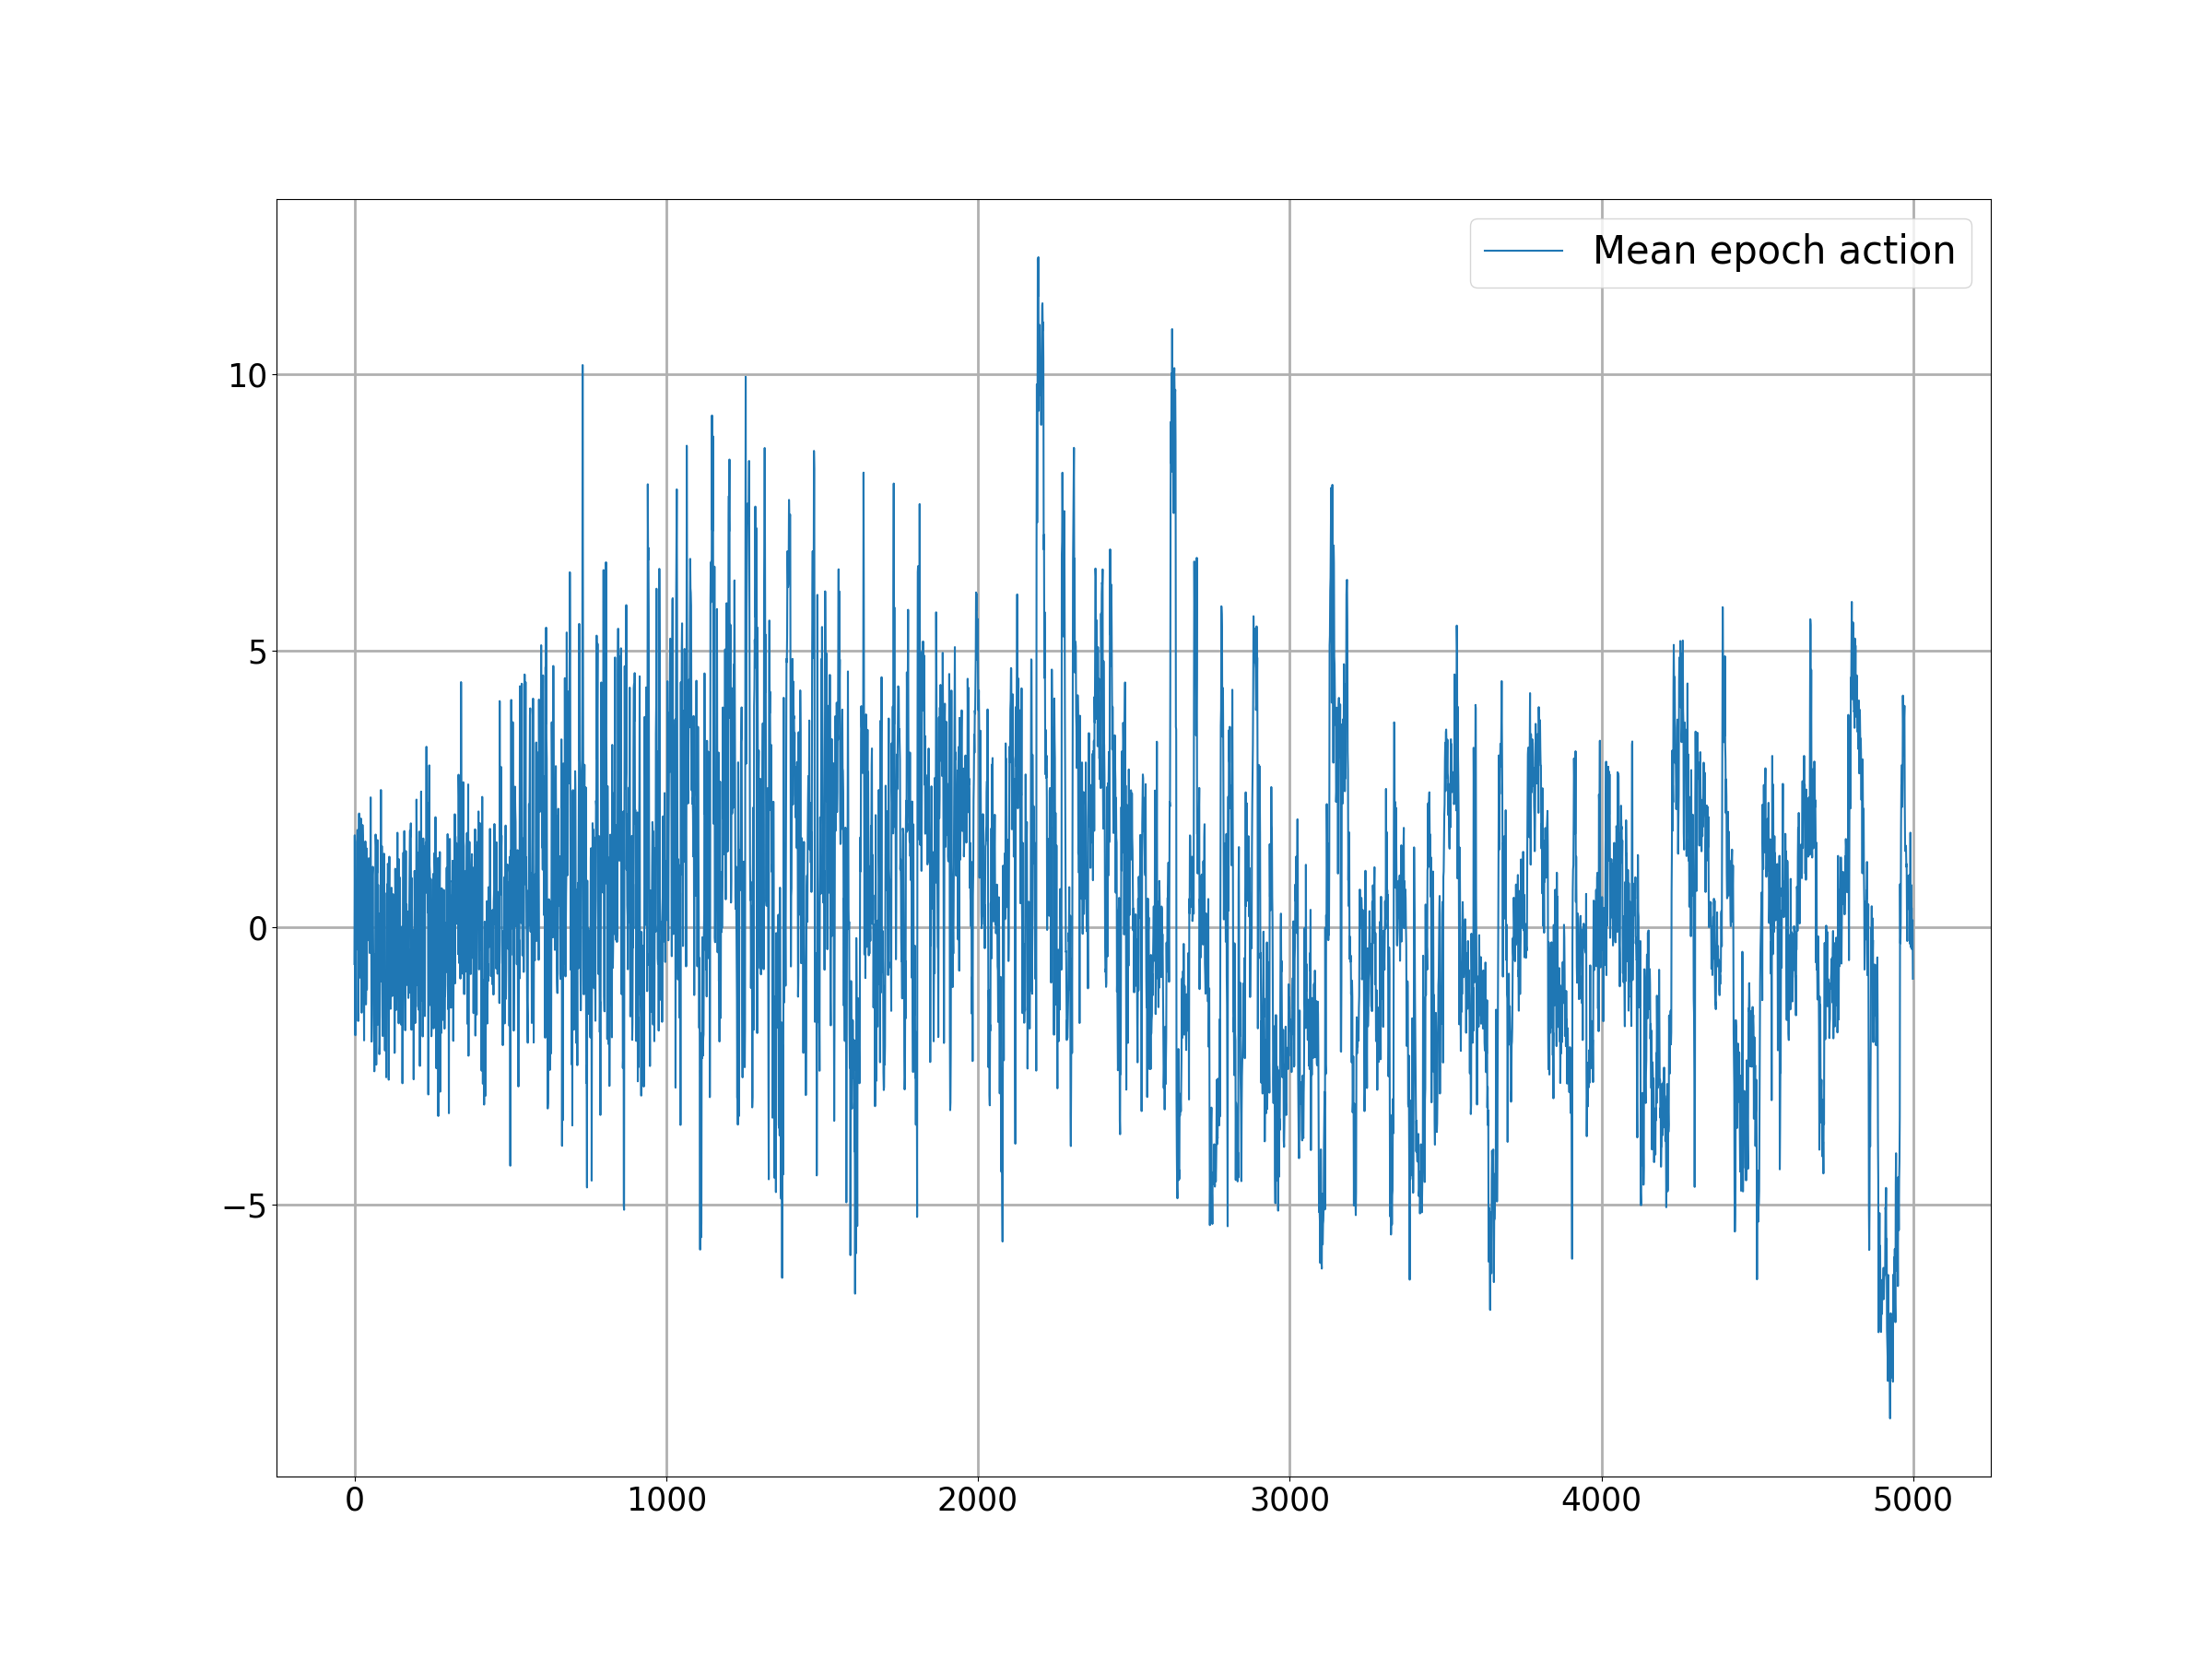
\includegraphics[width=\textwidth]{q_1_10000_SELL_mean_actions.png}
        \caption{Mean of actions per epoch (sell)}
        \label{fig:analysis-q-learn-1-action-sell}
    \end{subfigure}
    \caption{Mean rewards and actions for buying and selling on training data set I.}
    \label{fig:analysis-q-learn-1}
\end{figure}
\begin{figure}
    \centering
    \begin{subfigure}[b]{0.4\textwidth}
        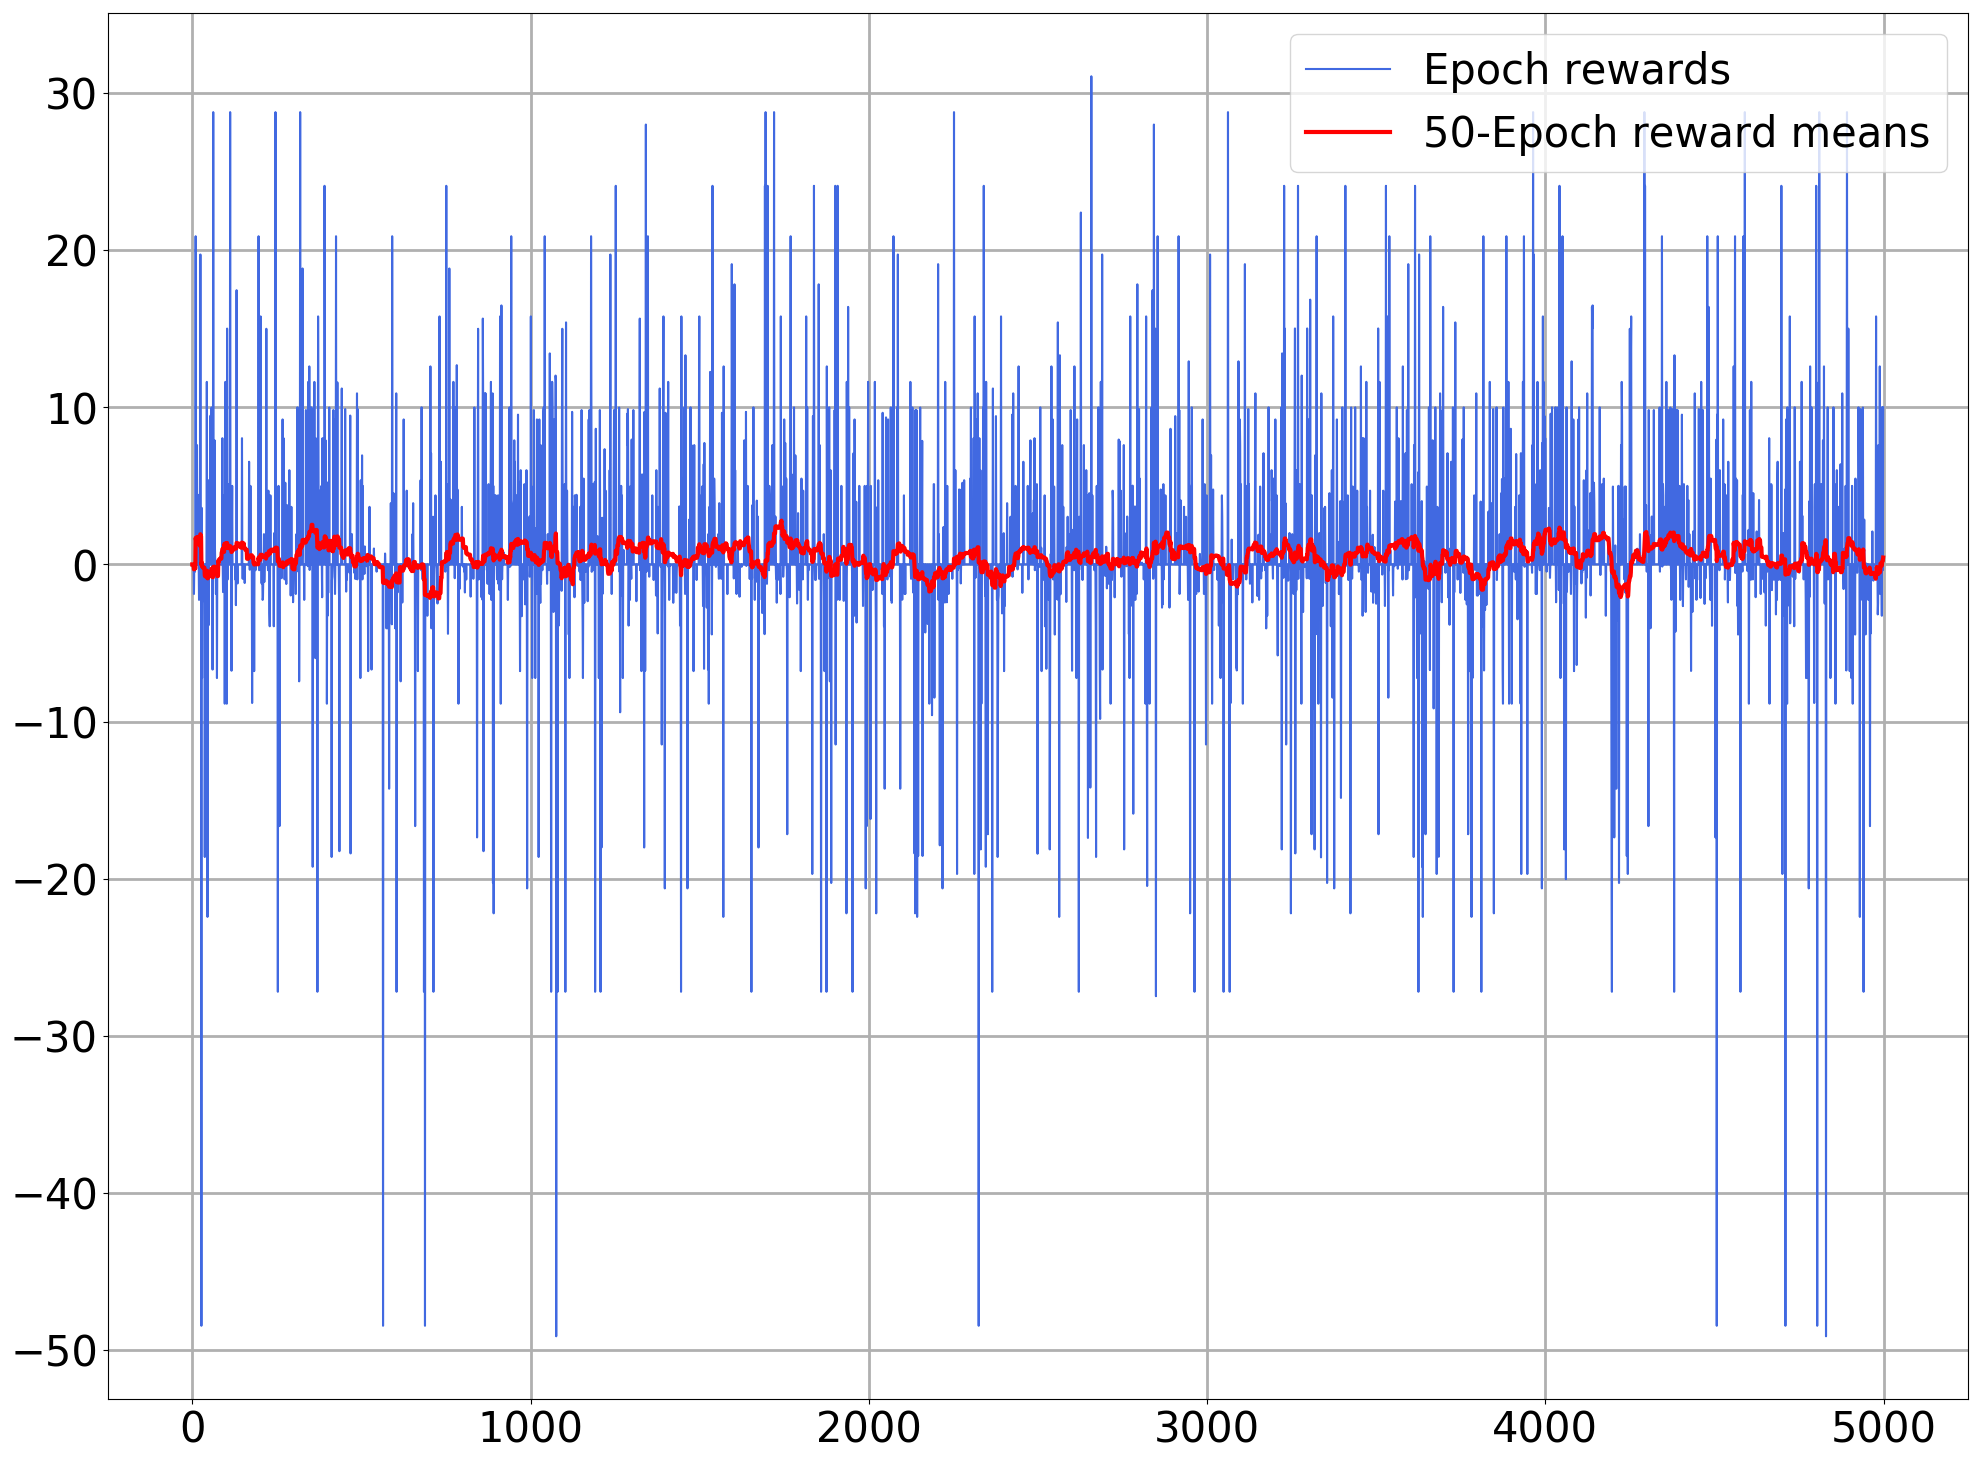
\includegraphics[width=\textwidth]{q_2_10000_BUY_rewards.png}
        \caption{Mean rewards per epoch (buy)}
        \label{fig:analysis-q-learn-2-reward-buy}
    \end{subfigure}
    \begin{subfigure}[b]{0.4\textwidth}
        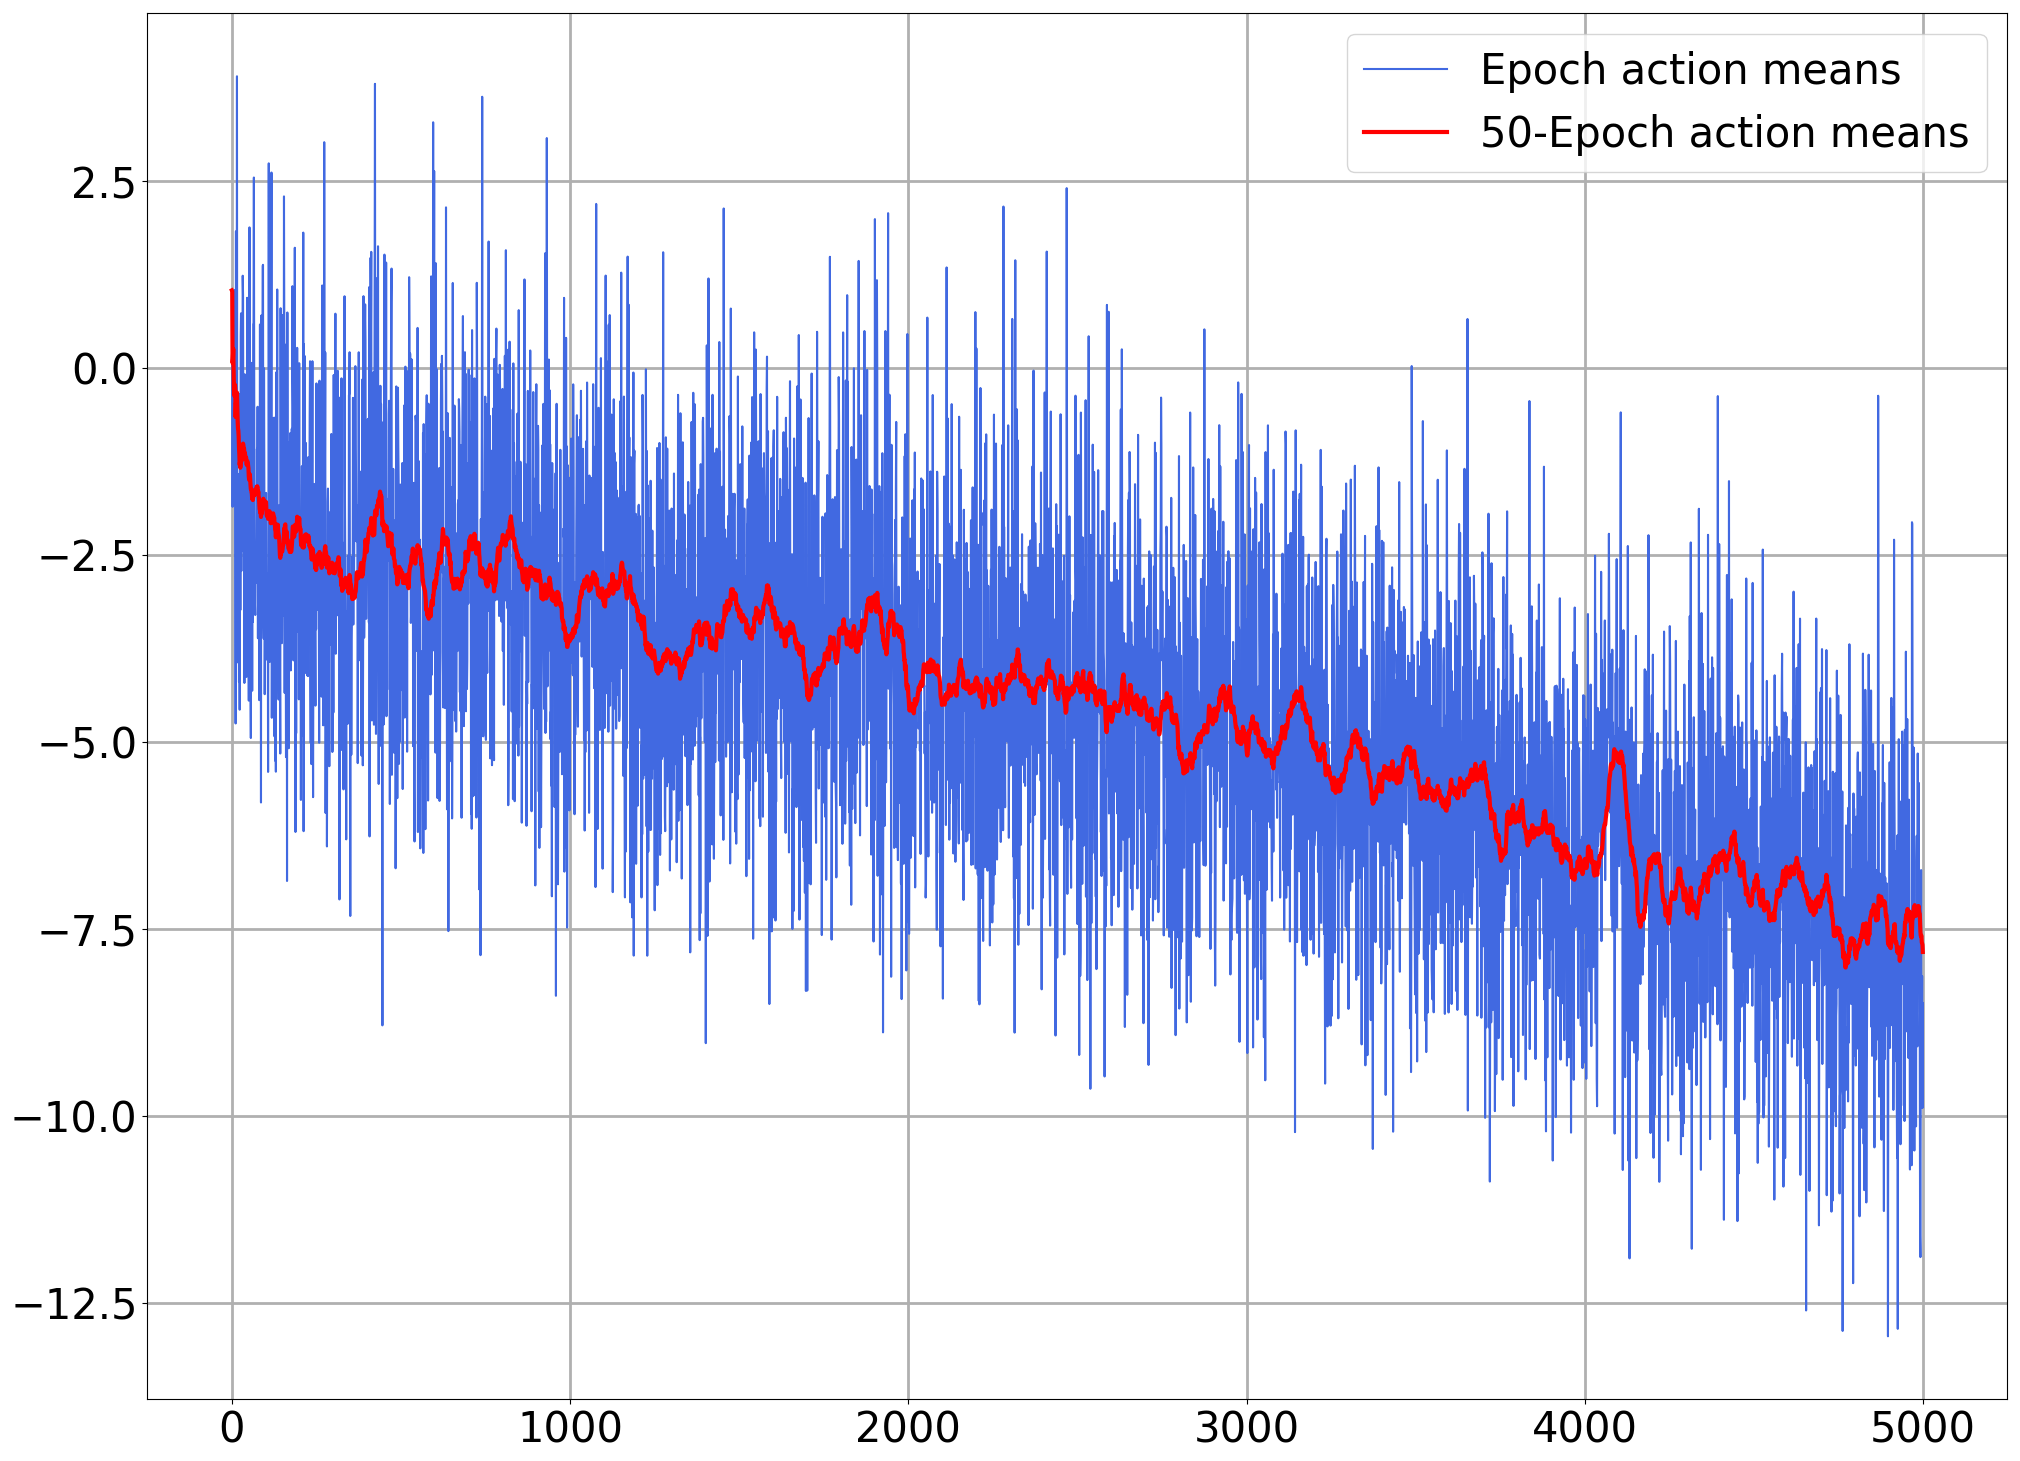
\includegraphics[width=\textwidth]{q_2_10000_BUY_mean_actions.png}
        \caption{Mean of actions per epoch (buy)}
        \label{fig:analysis-q-learn-2-action-buy}
    \end{subfigure}
    \begin{subfigure}[b]{0.4\textwidth}
        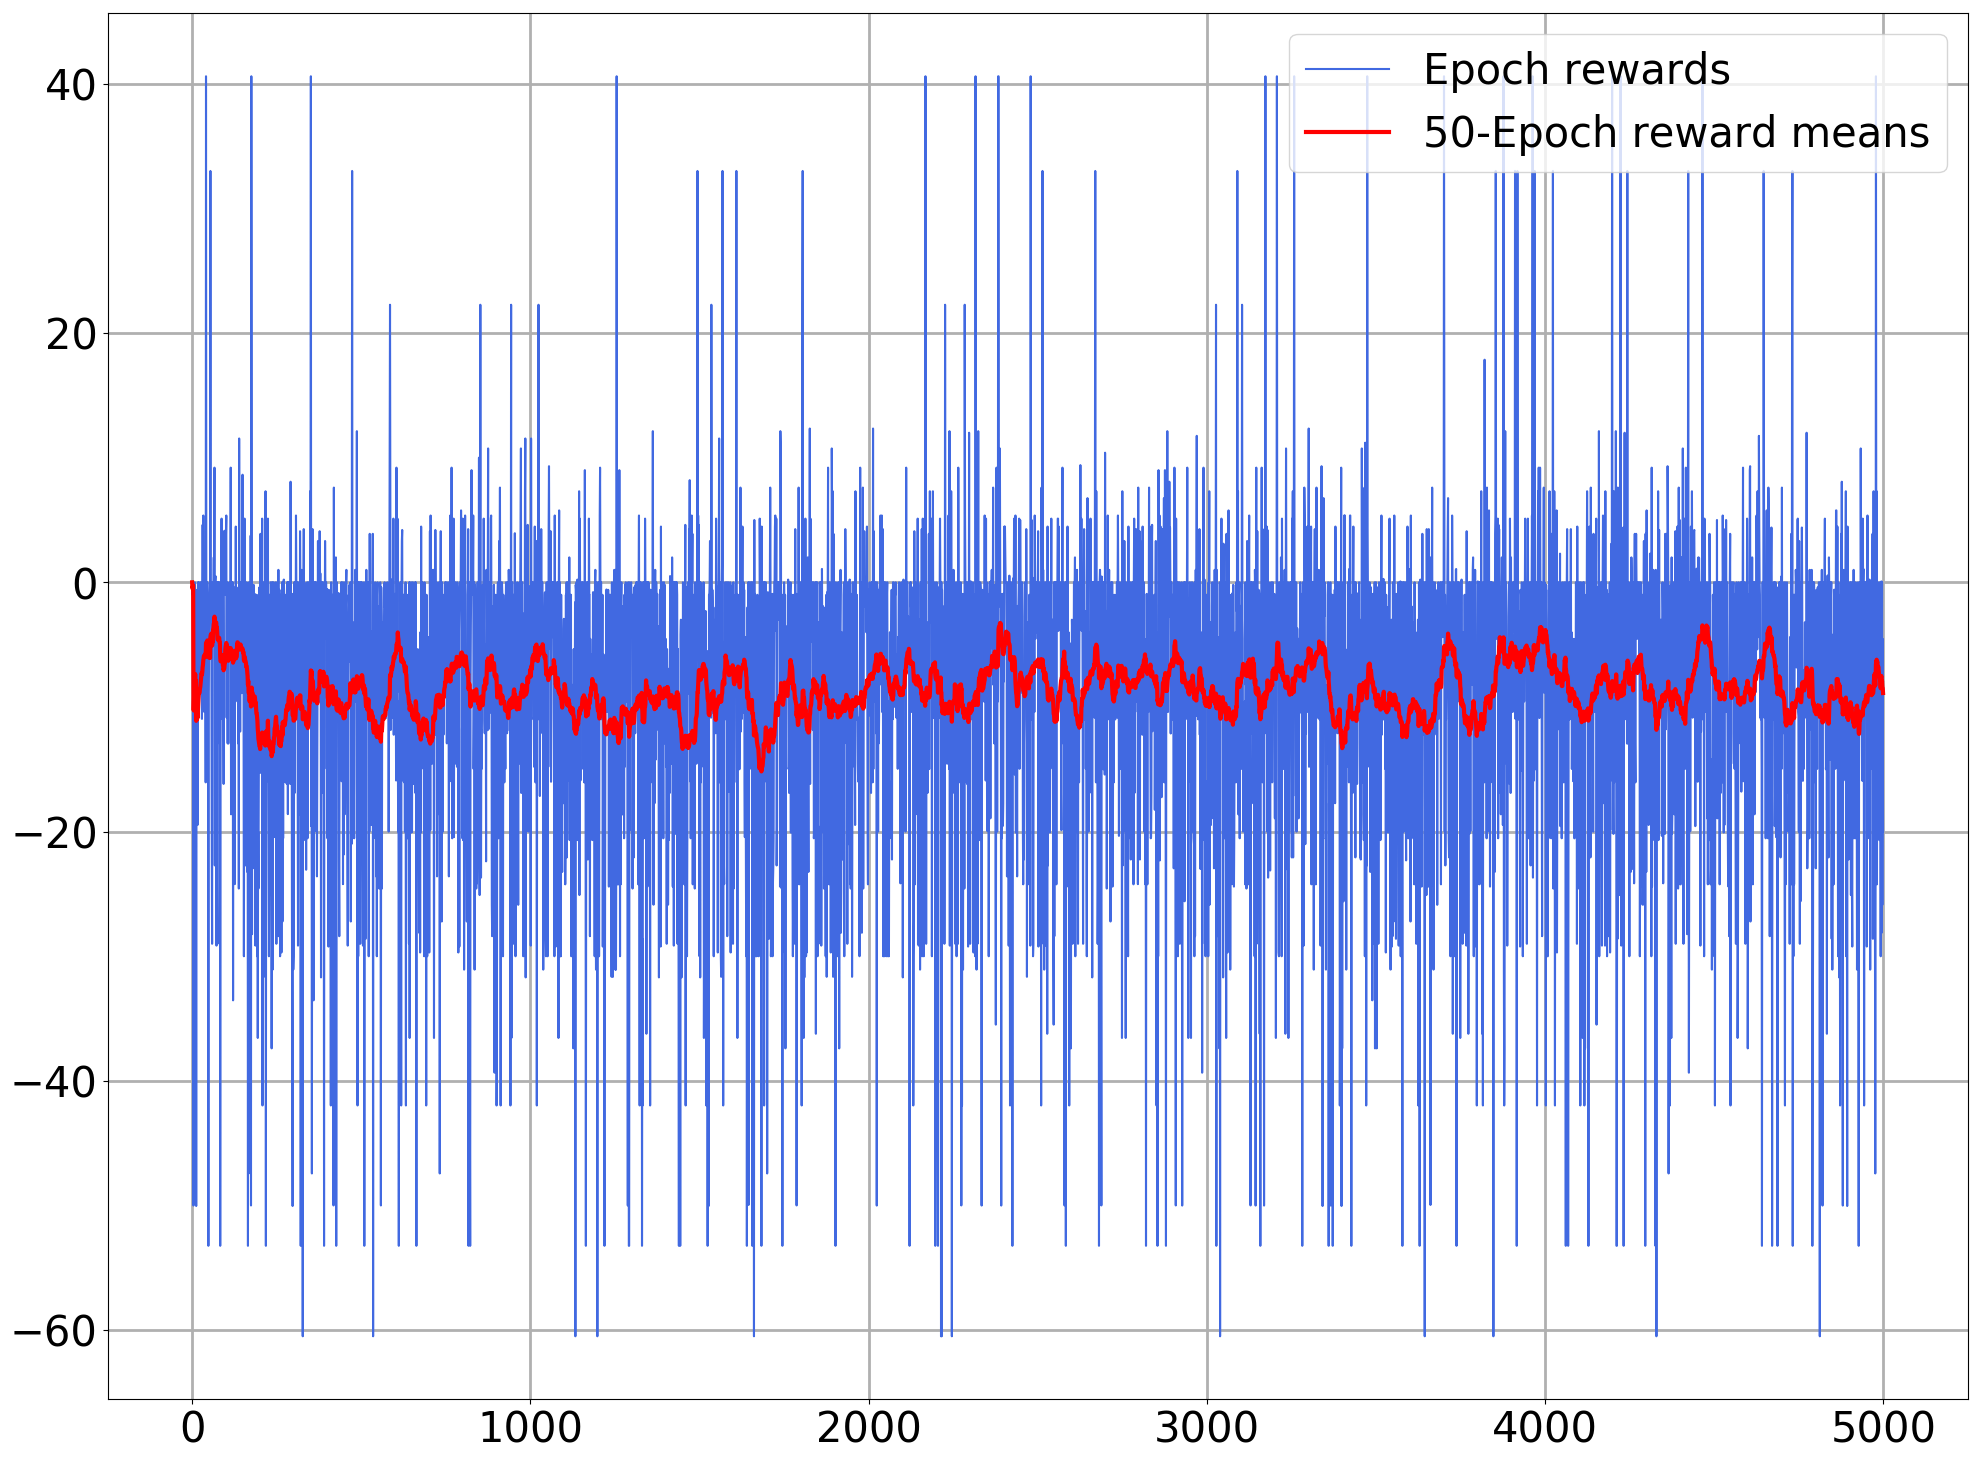
\includegraphics[width=\textwidth]{q_2_10000_SELL_rewards.png}
        \caption{Mean rewards per epoch (sell)}
        \label{fig:analysis-q-learn-2-reward-sell}
    \end{subfigure}
    \begin{subfigure}[b]{0.4\textwidth}
        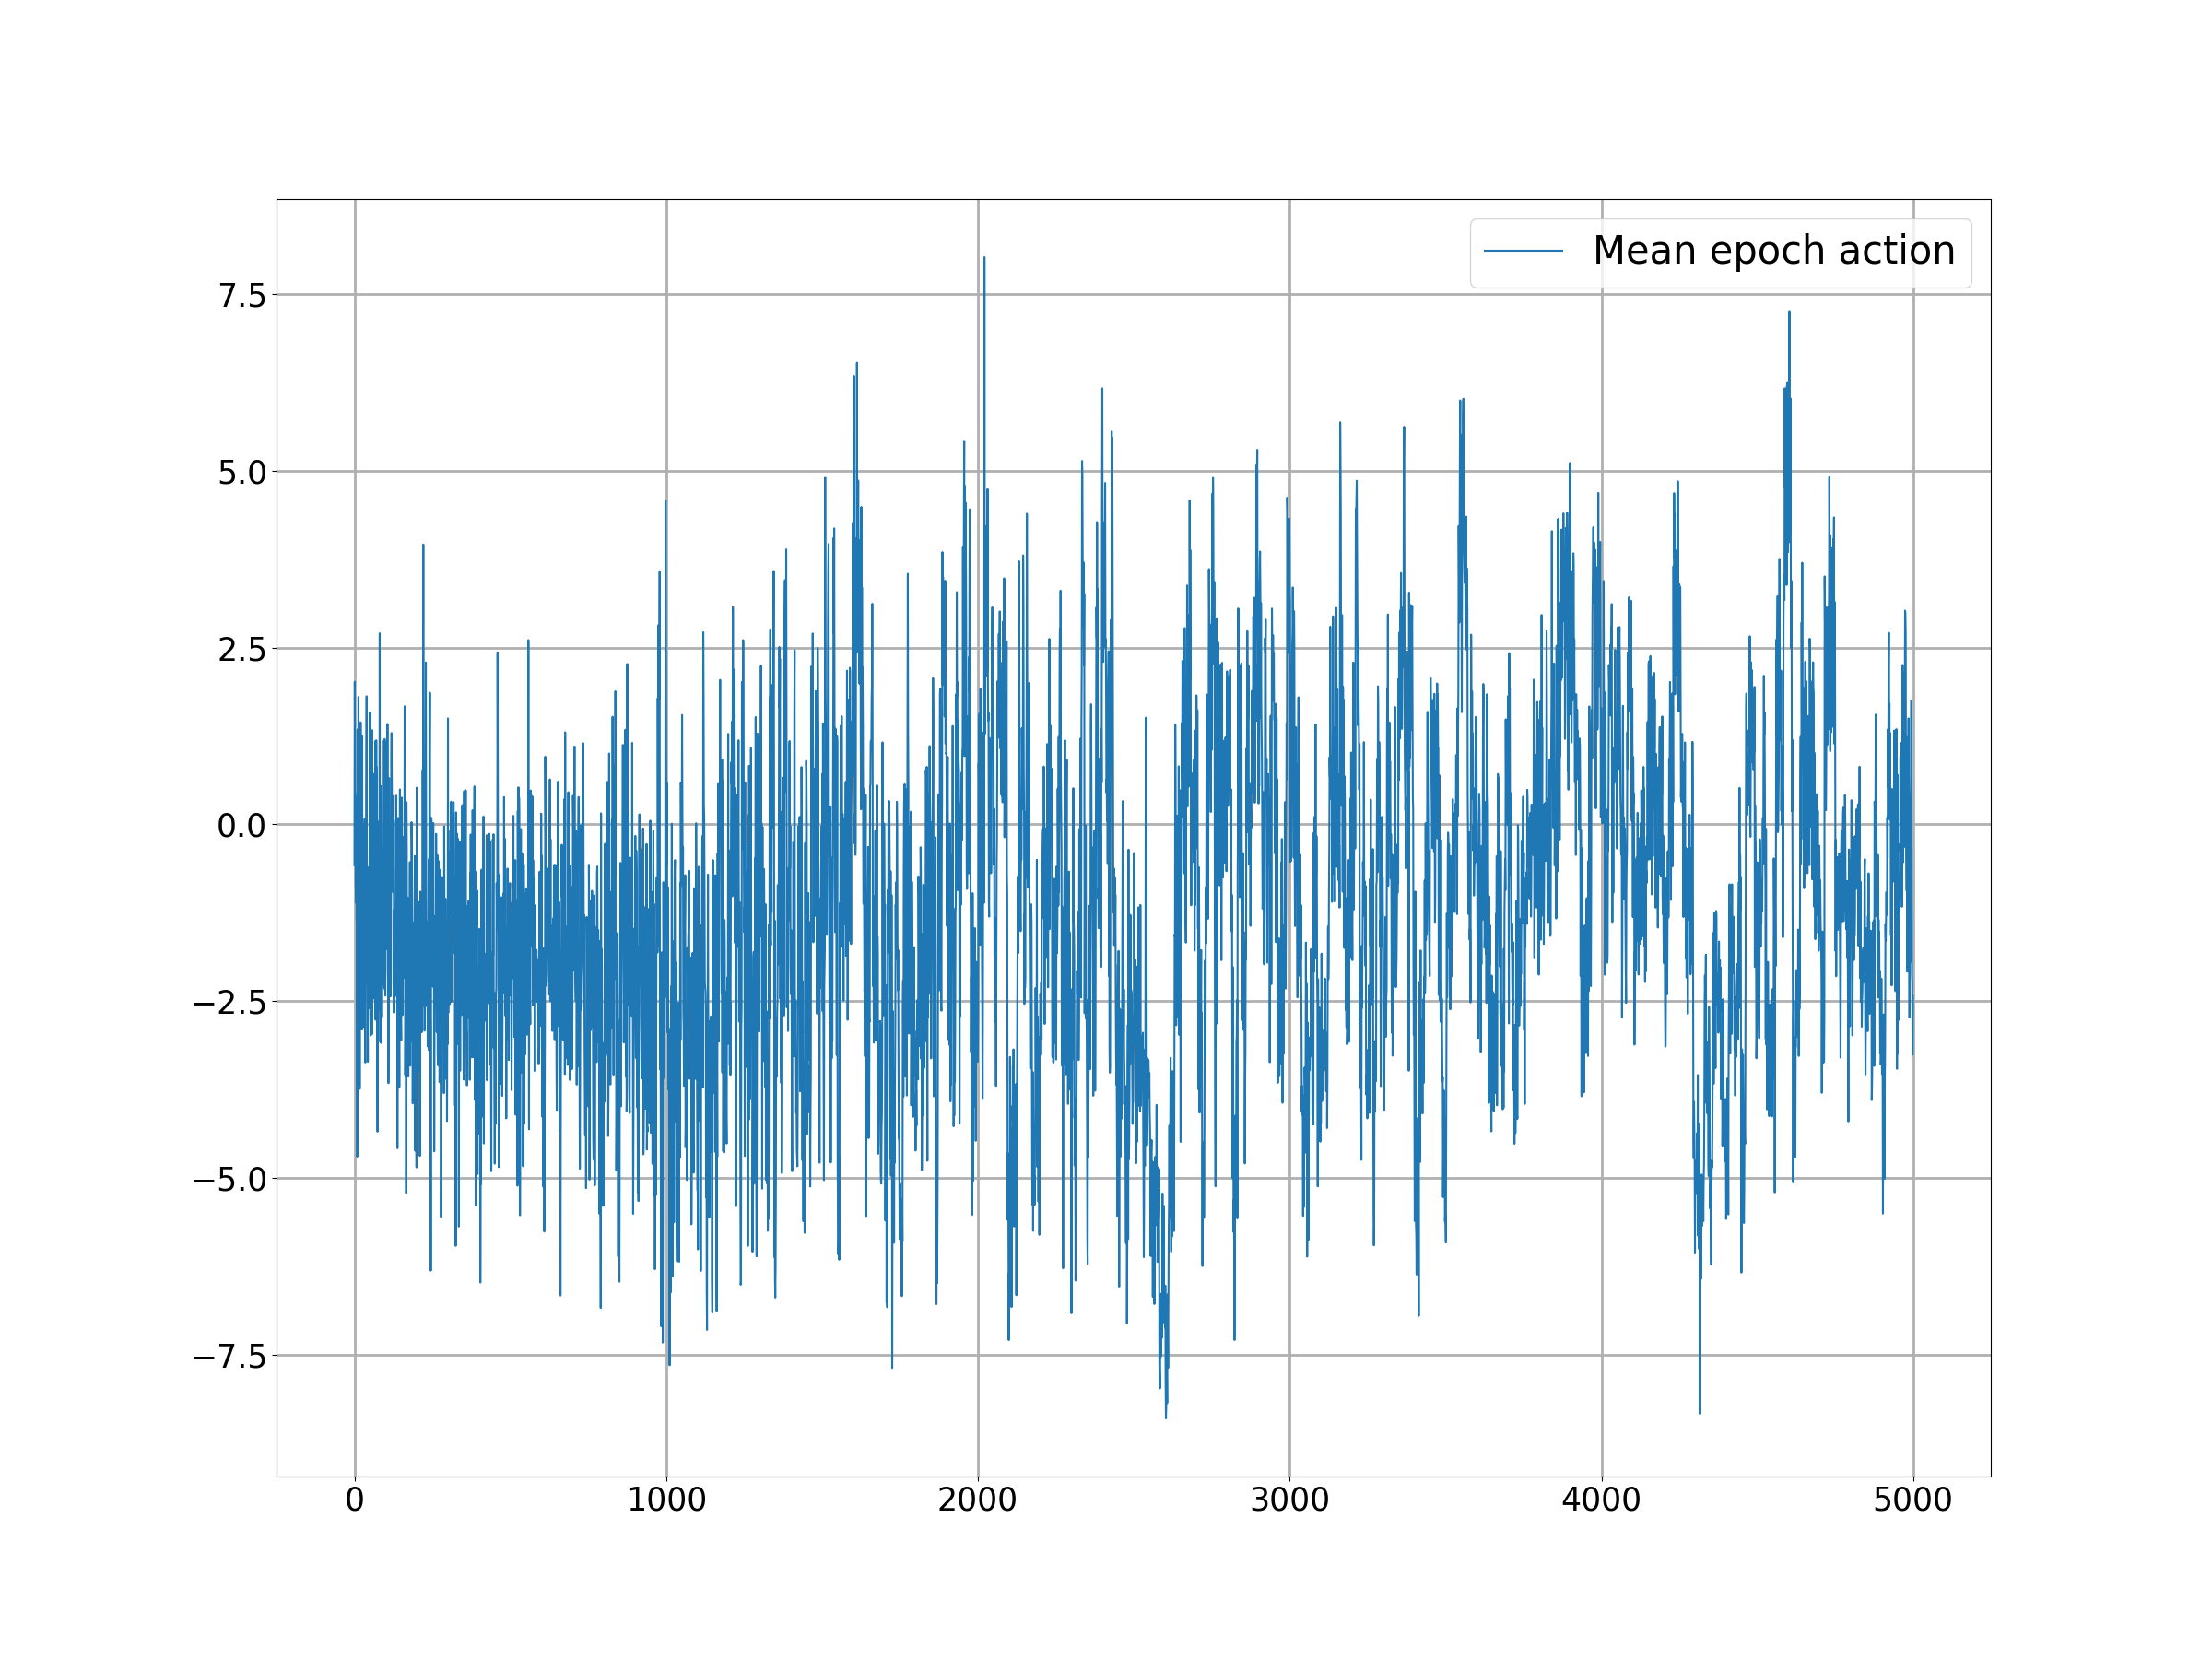
\includegraphics[width=\textwidth]{q_2_10000_SELL_mean_actions.png}
        \caption{Mean of actions per epoch (sell)}
        \label{fig:analysis-q-learn-2-action-sell}
    \end{subfigure}
    \caption{Mean rewards and actions for buying and selling on training data set II.}
    \label{fig:analysis-q-learn-2}
\end{figure}

Figure \ref{fig:analysis-q-learn-1} shows the training on data set I.
The average reward received during the training is shown in Figure \ref{fig:analysis-q-learn-1-reward-buy}.
Over the course of 5000 epochs, the agent was able to improve the mean reward by approximately $\sim$0.5, as a result of the changing policy.  This is illustrated in Figure \ref{fig:analysis-q-learn-1-action-buy}.
The agent started off with the average action of $\sim$-3, which is a result of the low epsilon parameter that makes the agent choose actions randomly.
Actions were then adjusted to the more negative side of the order book, such that after $\sim$1500 epochs, the agent chose actions as low as -20 and then adjusted and stagnated at $\sim$-15.
During the backtest, 1000 orders were executed on the test data set, which resulted in an average reward of \textit{-1.17}.
Making a comparison between the results of the empirical analysis performed on the same data set, as shown in Figure \ref{fig:behvaiour-down}, provides means for interpretation:
The policy learned by the Q-Learning agent performed worse than the expected costs of a market order, which was \$-1.12 when buying 1.0 BTC; this is shown in Section \ref{sec:eval-empirical}.
The highly negative average actions the agent choose toward the end of the training indicates that the order might not oftentimes have been able to be filled within the time horizon and an expensive market order had to follow.

The rewards received for the agents' tasks of selling the assets are much more volatile than for buying, as shown in Figure \ref{fig:analysis-q-learn-1-reward-sell}, and no clear improvement can be seen.
In addition, no significant adjustment was made by the agent regarding the mean of the actions chosen, as indicated in Figure \ref{fig:analysis-q-learn-1-action-sell}.
The backtest resulted in the achievement of an average reward of -21.34 by the agent.
The return received for placing market orders on the test set accounted to a negative reward of -27.70.
Hence, the agent was able to save \$6.36 when selling 1.0 BTC.
\\
\\
Figure \ref{fig:analysis-q-learn-2} shows the experiment performed on data set II.
The average reward received while training to buy the asset is shown in Figure \ref{fig:analysis-q-learn-2-reward-buy}.
Throughout the epochs, the agent was able to improve the mean reward by approximately 0.5, which was a similar result to that obtained with the previous data set (I), .
Even though the trend of this data set is the opposite, the change in chosen actions correlates to the previous findings and is illustrated in Figure \ref{fig:analysis-q-learn-2-action-buy}.
The backtest on test data set II resulted in an average reward of \textit{-1.04} --,  again worse than the average reward received with the training set.
A market order on test data set to accounted to an average reward of -1.06, indicating that the agent's policy was saving \$0.02 when buying 1.0 BTC.
On the basis of the empirical analysis performed when buying on this data set, as shown in Figure \ref{fig:behvaiour-up}, and comparing it to the rewards received by the agent, implies that the agent failed to execute orders with the limit orders placed and oftentimes market orders were followed.

As with the sell orders placed on data set I, the rewards received from the agent's tasks to sell the assets in data set II are very volatile, as shown in Figure \ref{fig:analysis-q-learn-1-reward-sell}.
No improvement can be seen from the rewards during the training and no significant adjustment was made by the agent regarding the actions chosen, as indicated in Figure \ref{fig:analysis-q-learn-2-action-sell}.
The backtest resulted in an average reward of -4.74 achieved by the agent, whereas market orders are expected to result in an average reward of -1.72.
Hence, the use of an requires the payment of a premium of \$3.02 when selling 1.0 BTC.

\subsection{Conclusion of Q-Learning approach}

\begin{table}[H]
\centering
\begin{tabular}{l|l|l|}
\cline{2-3}
& \textbf{Q-Learner} & \textbf{\begin{tabular}[c]{@{}l@{}}$\mathbb{E}$[Market\\ Order]\end{tabular}} \\ \hline
\multicolumn{1}{|l|}{\textbf{Buy (I)}}   & -1.17          & -0.05                                                           \\ \hline
\multicolumn{1}{|l|}{\textbf{Sell (I)}}  & -21.34         & -27.70                                                          \\ \hline
\multicolumn{1}{|l|}{\textbf{Buy (II)}}  & -1.04          & -1.06                                                           \\ \hline
\multicolumn{1}{|l|}{\textbf{Sell (II)}} & -4.74          & -1.72                                                           \\ \hline
\multicolumn{1}{|l|}{\textbf{$\Sigma$}} & -28.29          & -30.53                                                           \\ \hline
\end{tabular}
\caption{Summary of rewards for the Q-Learning agent and market orders.}
\label{tbl:analysis-q-learn-summary}
\end{table}
The findings of this section are summarized in Table \ref{tbl:analysis-q-learn-summary}.
We conclude that the Q-Learning agent was not able to constantly place buy and sell orders in a way which would result in a price better than the current market price.
Oftentimes, a market order, which would trigger an immediate purchase or sale, would be the better choice.
Clearly, this is due to the fact that the agent was not able to find the most suitable actions.
Furthermore, in order to investigate whether or not these findings were a result of the agent aiming for a reward that was too immediate, the same experiment was performed with $\gamma=0.3$ and therefore rely more extensively on the future rewards.
However, no improvement could be achieved and instead, the agent achieved similar rewards while requiring more epochs in order to converge to the same mean of actions.
In this section, we have only investigated the mean of the actions chosen throughout an epoch, which has provided evidence, which we regard as sufficient, that the chosen actions resulted mostly in market orders.
Furthermore, it is to be assumed that the absence of market variables makes it hard for any learner to determine an optimal policy.
Therefore, the following section will make use of market variables in order to determine whether or not a learner can exploit the information hidden in the market and therefore act in favor of optimally placing limit orders.

\section{Deep Q-Network with market features}
\label{sec:eval-dqn}
In the previous section, the Q-Learning agent was trained on data sets I and II, and no significant optimization in terms of the buying and selling of assets was achieved.
By considering the above-mentioned results of the empirical analysis of the limit order placement behavior, we found that most of the limit orders placed by the Q-Learning agent were not filled within the given time horizon and instead, market orders had to be submitted after the time has elapsed.

In this section, we aim to determine whether or not the DQN agent is capable of extracting information provided by the raw market features and therefore improve the limit order placement policy.
The setup is the same as in the previous section, where the agents task is to buy and sell 1.0 BTC within 100 seconds with discrete step size $\Delta{t}=10$ in both data sets I and II.
Furthermore, both of the features constructed in Chapter \ref{chap:data}, will be applied and investigated separately.
The input shape of the model in use that approximates the action-value function, as described in Chapter \ref{chap:preliminaries} (Section \ref{sec:deep-reinforcement-learning}), is determined by the feature in use and is described below.
We evaluate the performance of the DQN agent under the application of both neural network architectures, the standard convolutional neural network and the multilayer perceptron, as presented in Section \ref{setup:dqn}.
For both of these DQN agent setups, we rely on the default hyperparameters worked out by Mnih et al. \cite{mnih2015human}, as shown in Figure \ref{fig:eval-dqn-hyperparameters}.
Furthermore, we will train both agents with 5000 epochs and will test with 1000 epochs.
Finally, we will conclude our findings and determine the capabilities of the DQN approach (and its use of the market features) by comparing it to the expected returns for a market order calculated earlier in Section \ref{sec:eval-empirical}.
\begin{figure}[H]
    \centering
    \makebox[\linewidth]{
        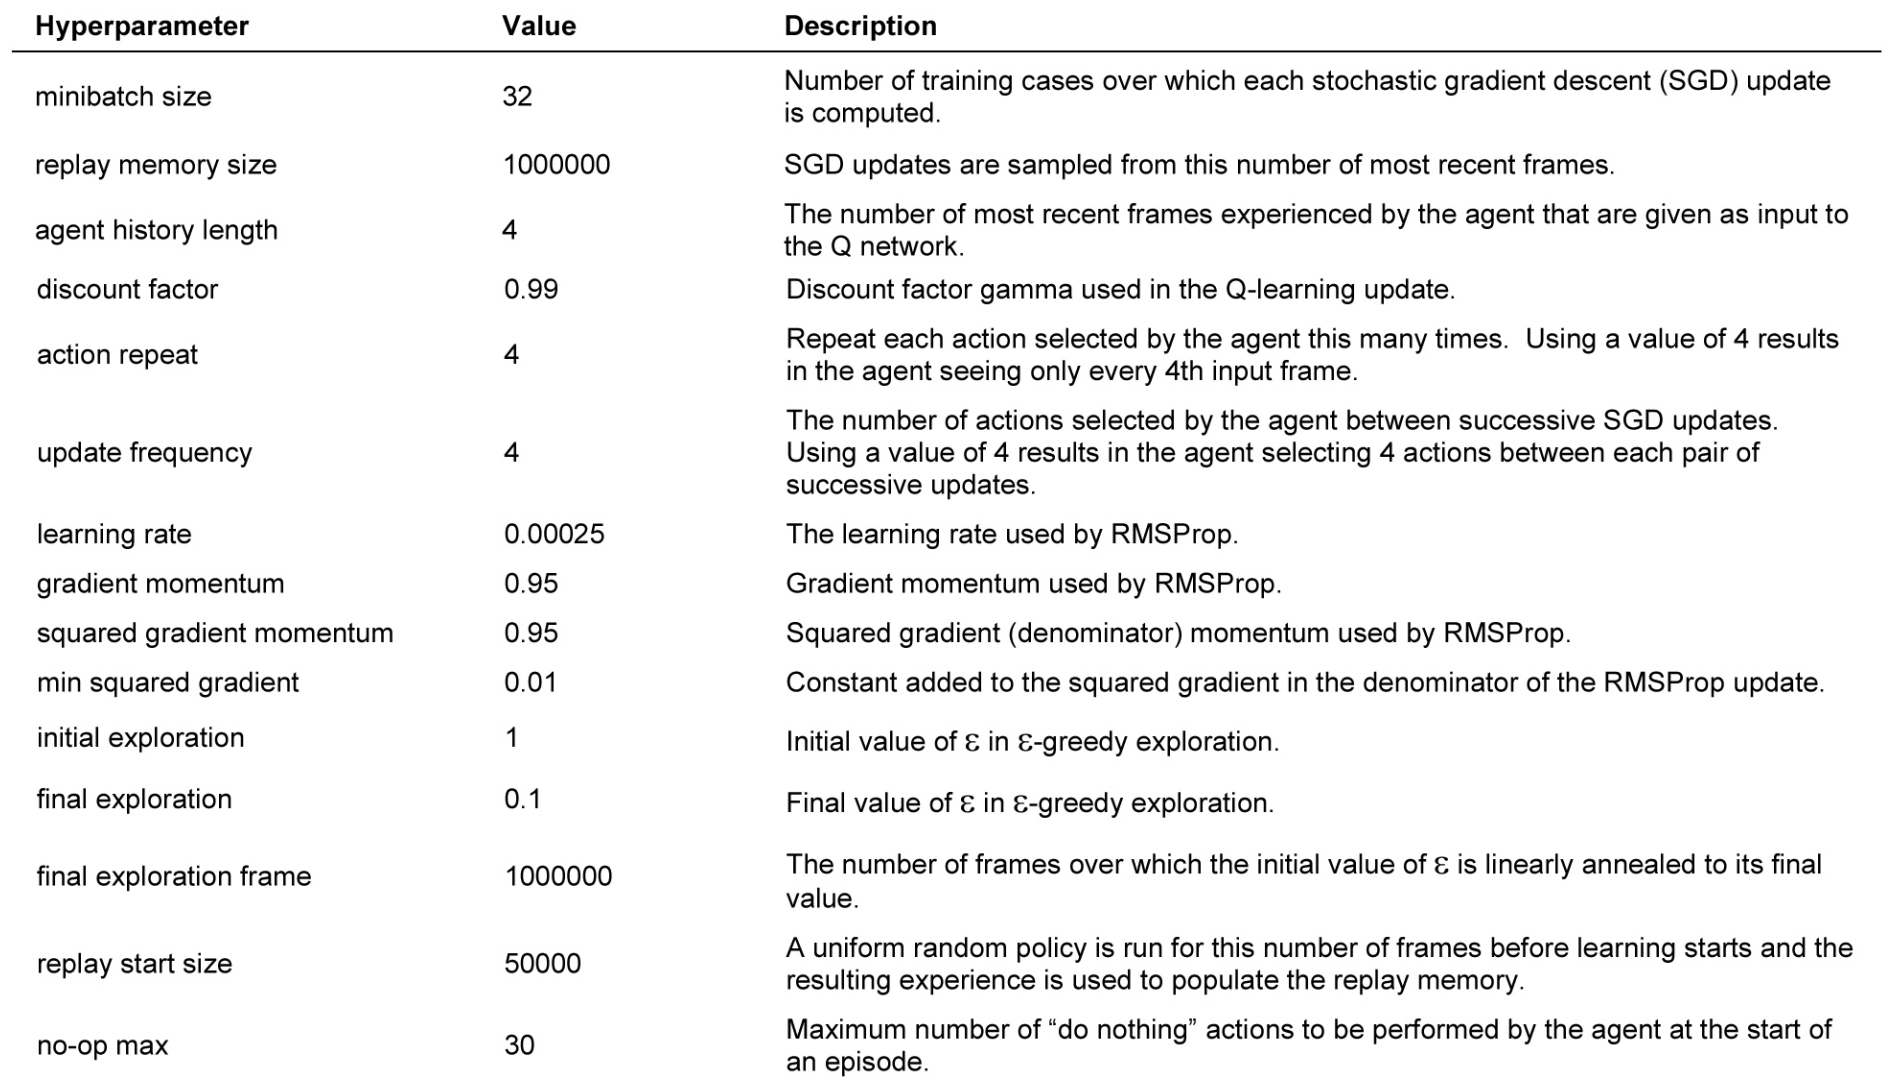
\includegraphics[width=14cm]{images/dqn_hyperparameters.png}
    }
    \caption{The values of all the hyperparameters were selected. We did not perform a systematic grid search owing to the high computational cost, although it is conceivable that better results can be obtained by tuning these hyperparameter values.}
    \label{fig:eval-dqn-hyperparameters}
\end{figure}

\subsection{Application of historical order feature}

The following evaluation of the DQN agent setups that consider Feature I, as described in Chapter \ref{chap:data} (Section \ref{sec:data-feature-1}).
Furthermore, in this initial run we consider $m=30$ historical order book states, alongside the maximum number of bid and ask levels $n=40$.
This results in a feature set size of $(60, 40, 2)$, as a consequence of the defined size $(2*m, n, 2)$.
When we included the two private variables by appending a vector $[inventory, time]$ at the beginning of this feature vector, the size of the feature set was $(61, 40, 2)$ and, as such, will serve as the input for the neural networks in use.

\begin{figure}[H]
    \centering
    \begin{subfigure}[b]{0.4\textwidth}
        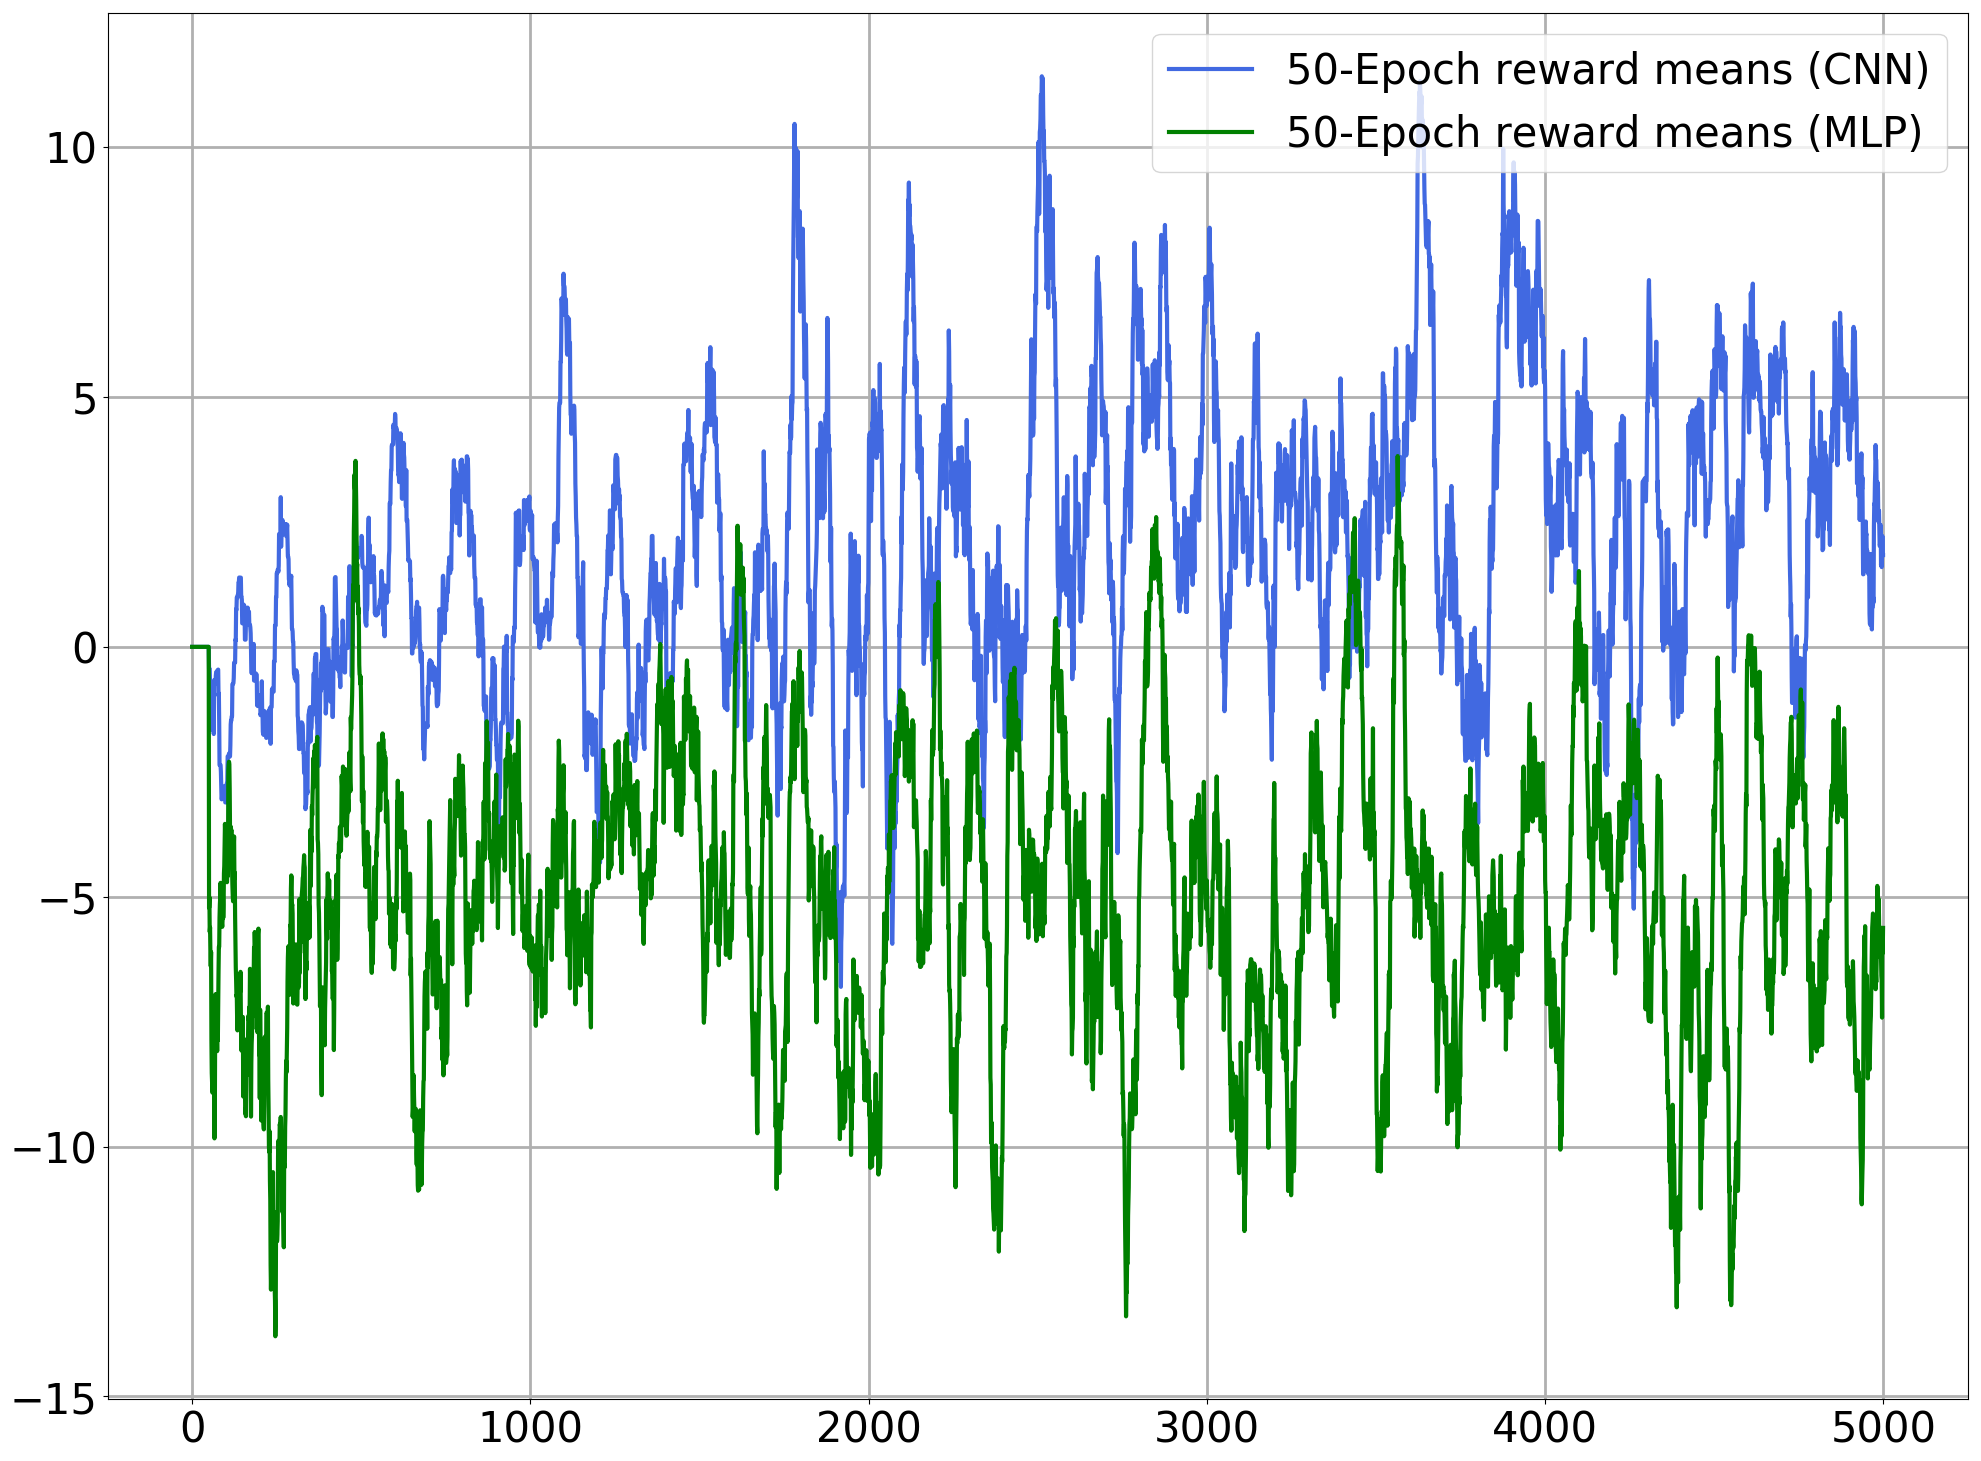
\includegraphics[width=\textwidth]{cnn_nn_1_buy_bidask_rewards.png}
        \caption{Reward per epoch (buy)}
        \label{fig:analysis-dqn-1-reward-buy}
    \end{subfigure}
    \begin{subfigure}[b]{0.4\textwidth}
        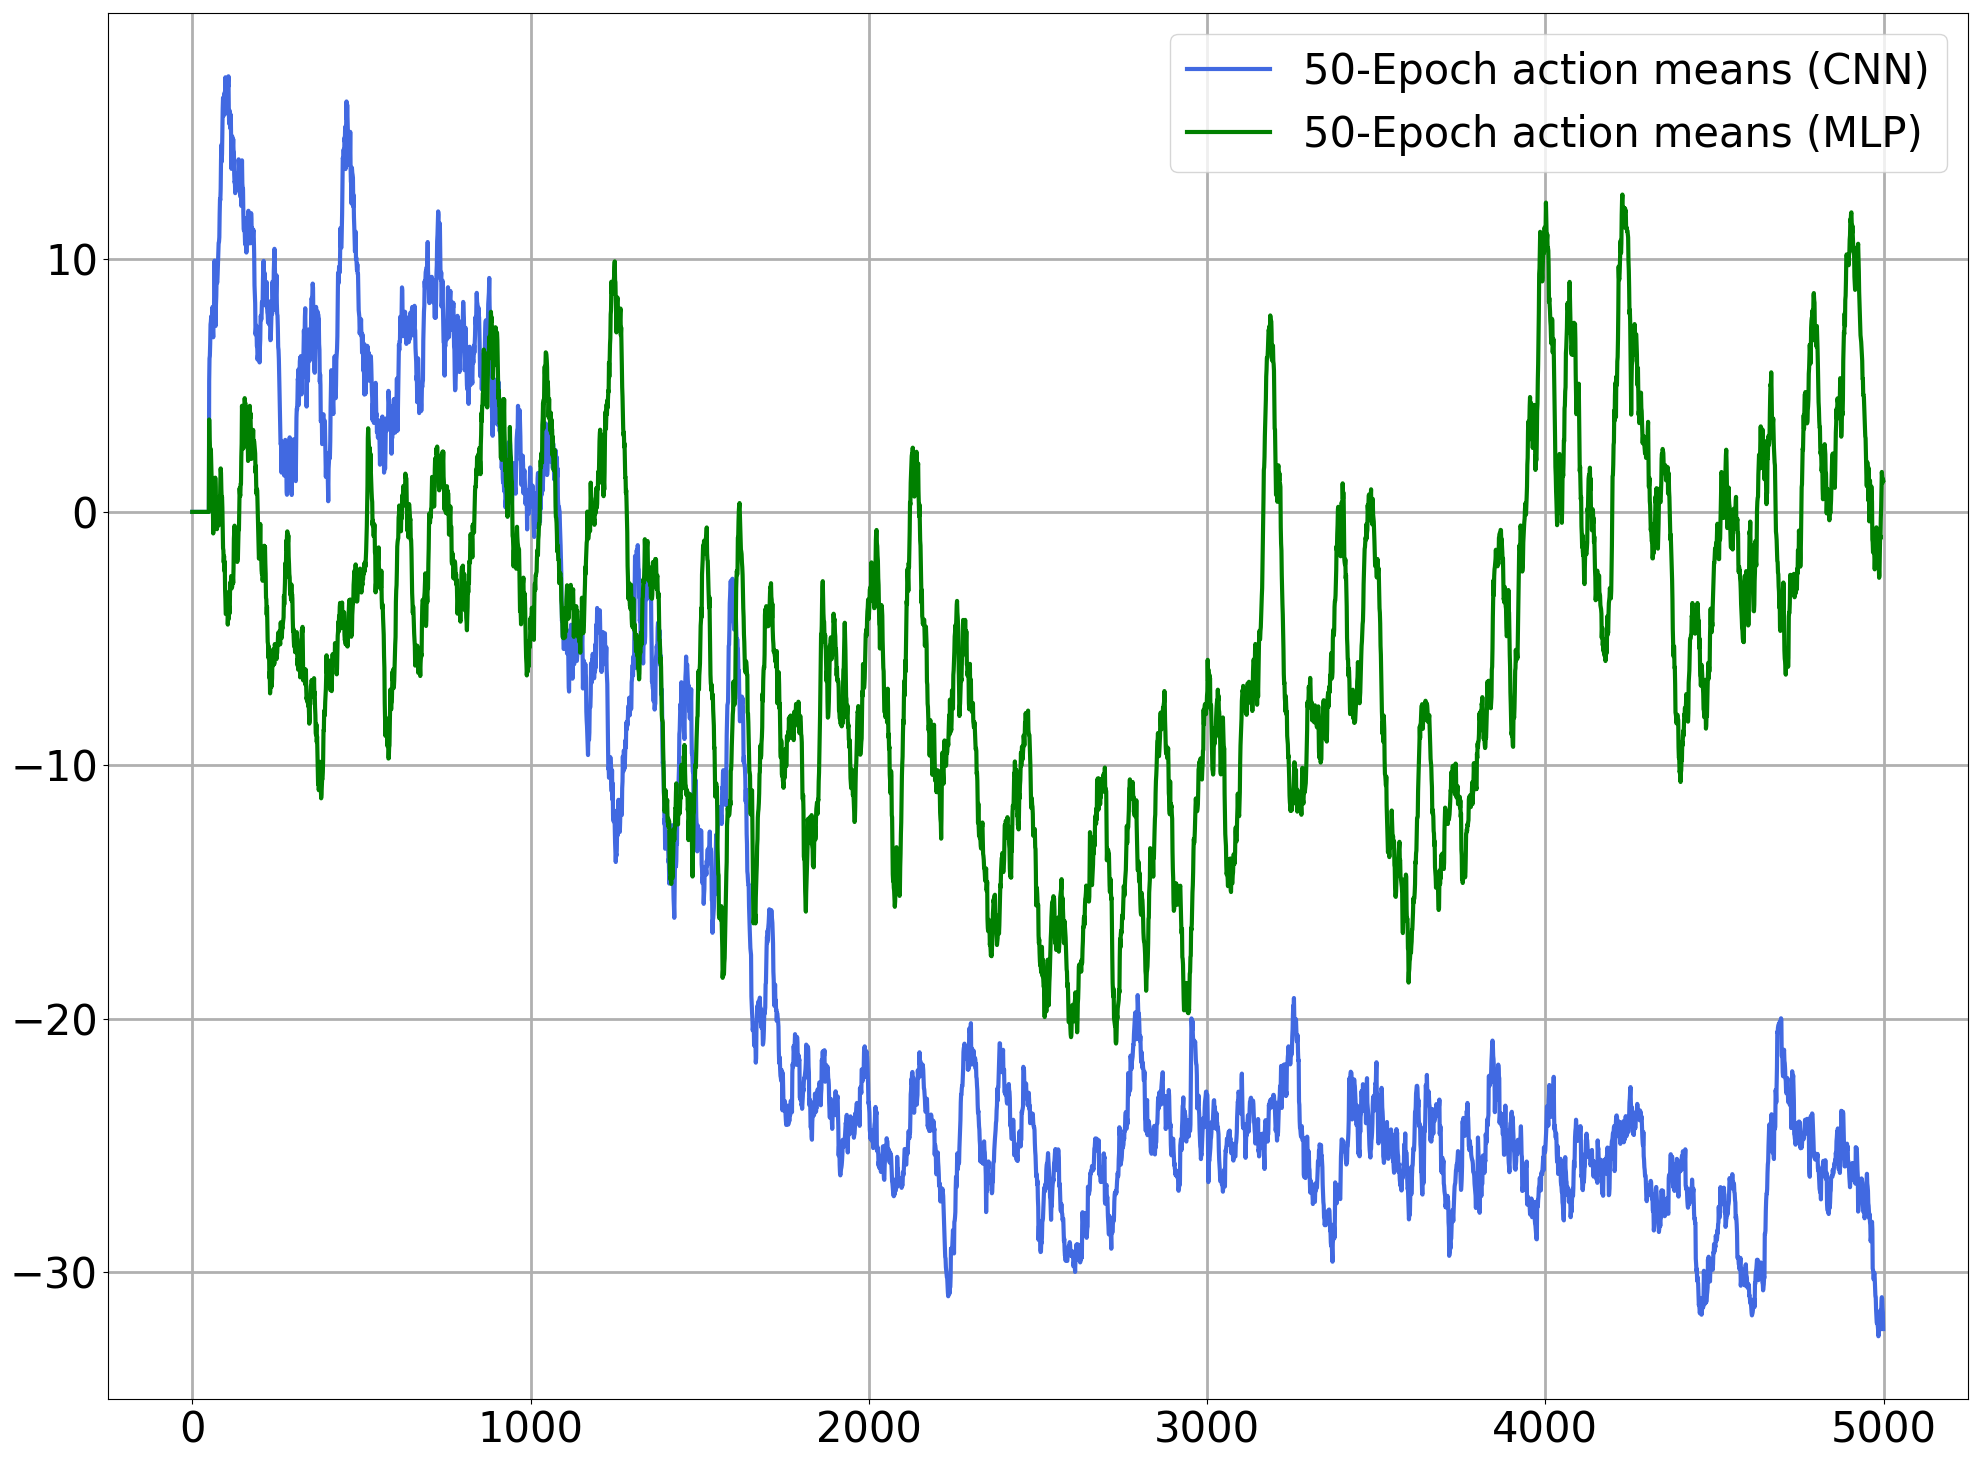
\includegraphics[width=\textwidth]{cnn_nn_1_buy_bidask_mean_actions.png}
        \caption{Mean of actions per epoch (buy)}
        \label{fig:analysis-dqn-1-action-buy}
    \end{subfigure}
    \begin{subfigure}[b]{0.4\textwidth}
        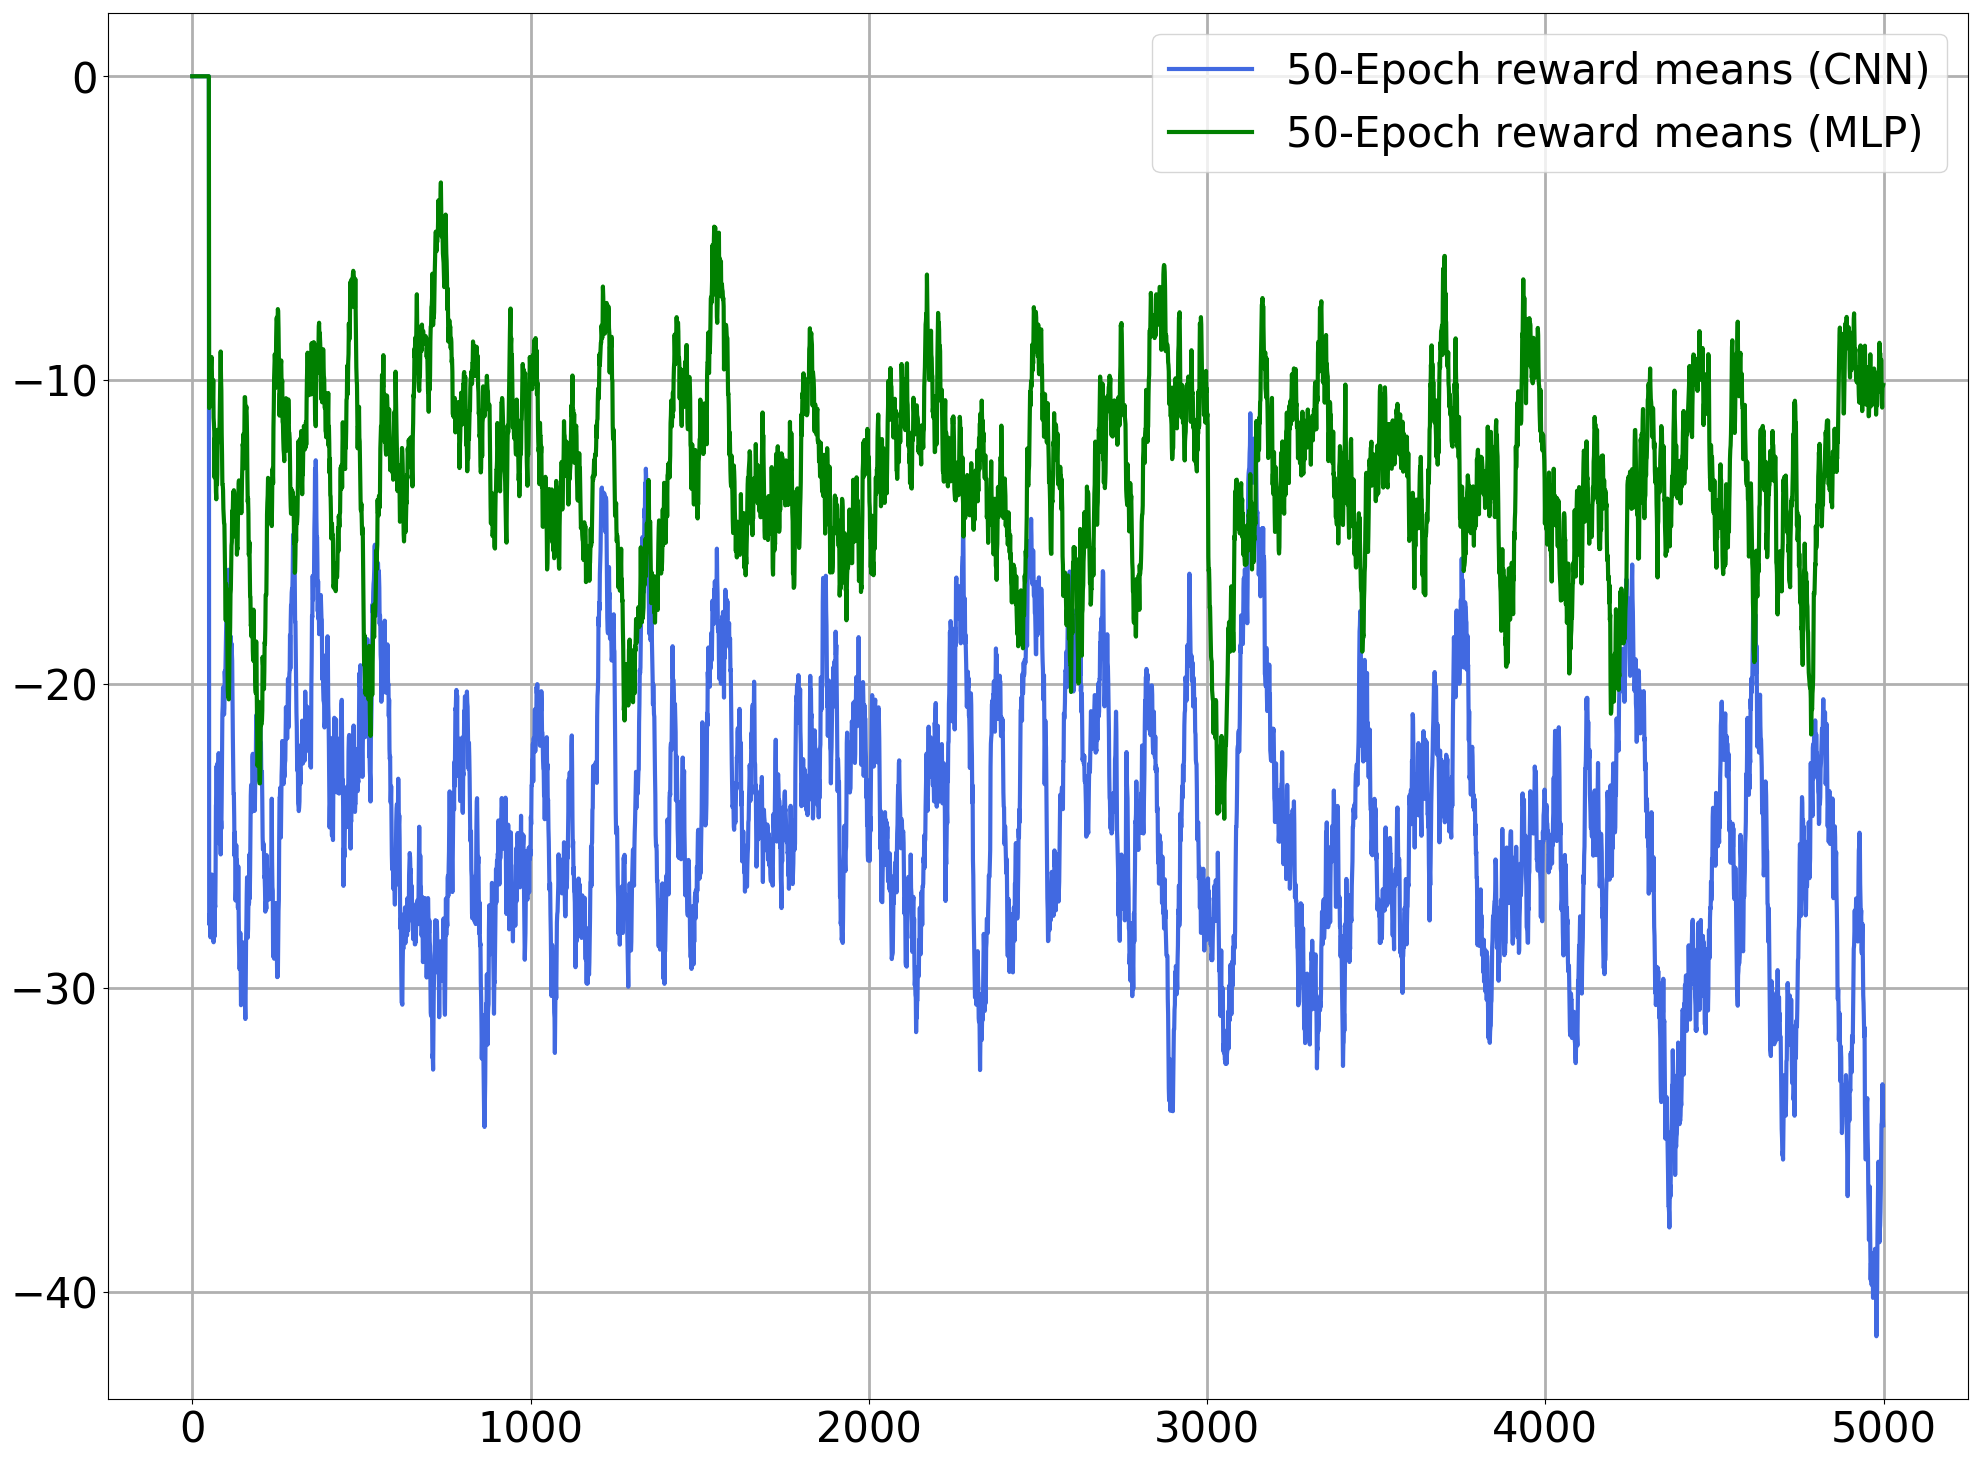
\includegraphics[width=\textwidth]{cnn_nn_1_sell_bidask_rewards.png}
        \caption{Mean rewards per epoch (sell)}
        \label{fig:analysis-dqn-1-reward-sell}
    \end{subfigure}
    \begin{subfigure}[b]{0.4\textwidth}
        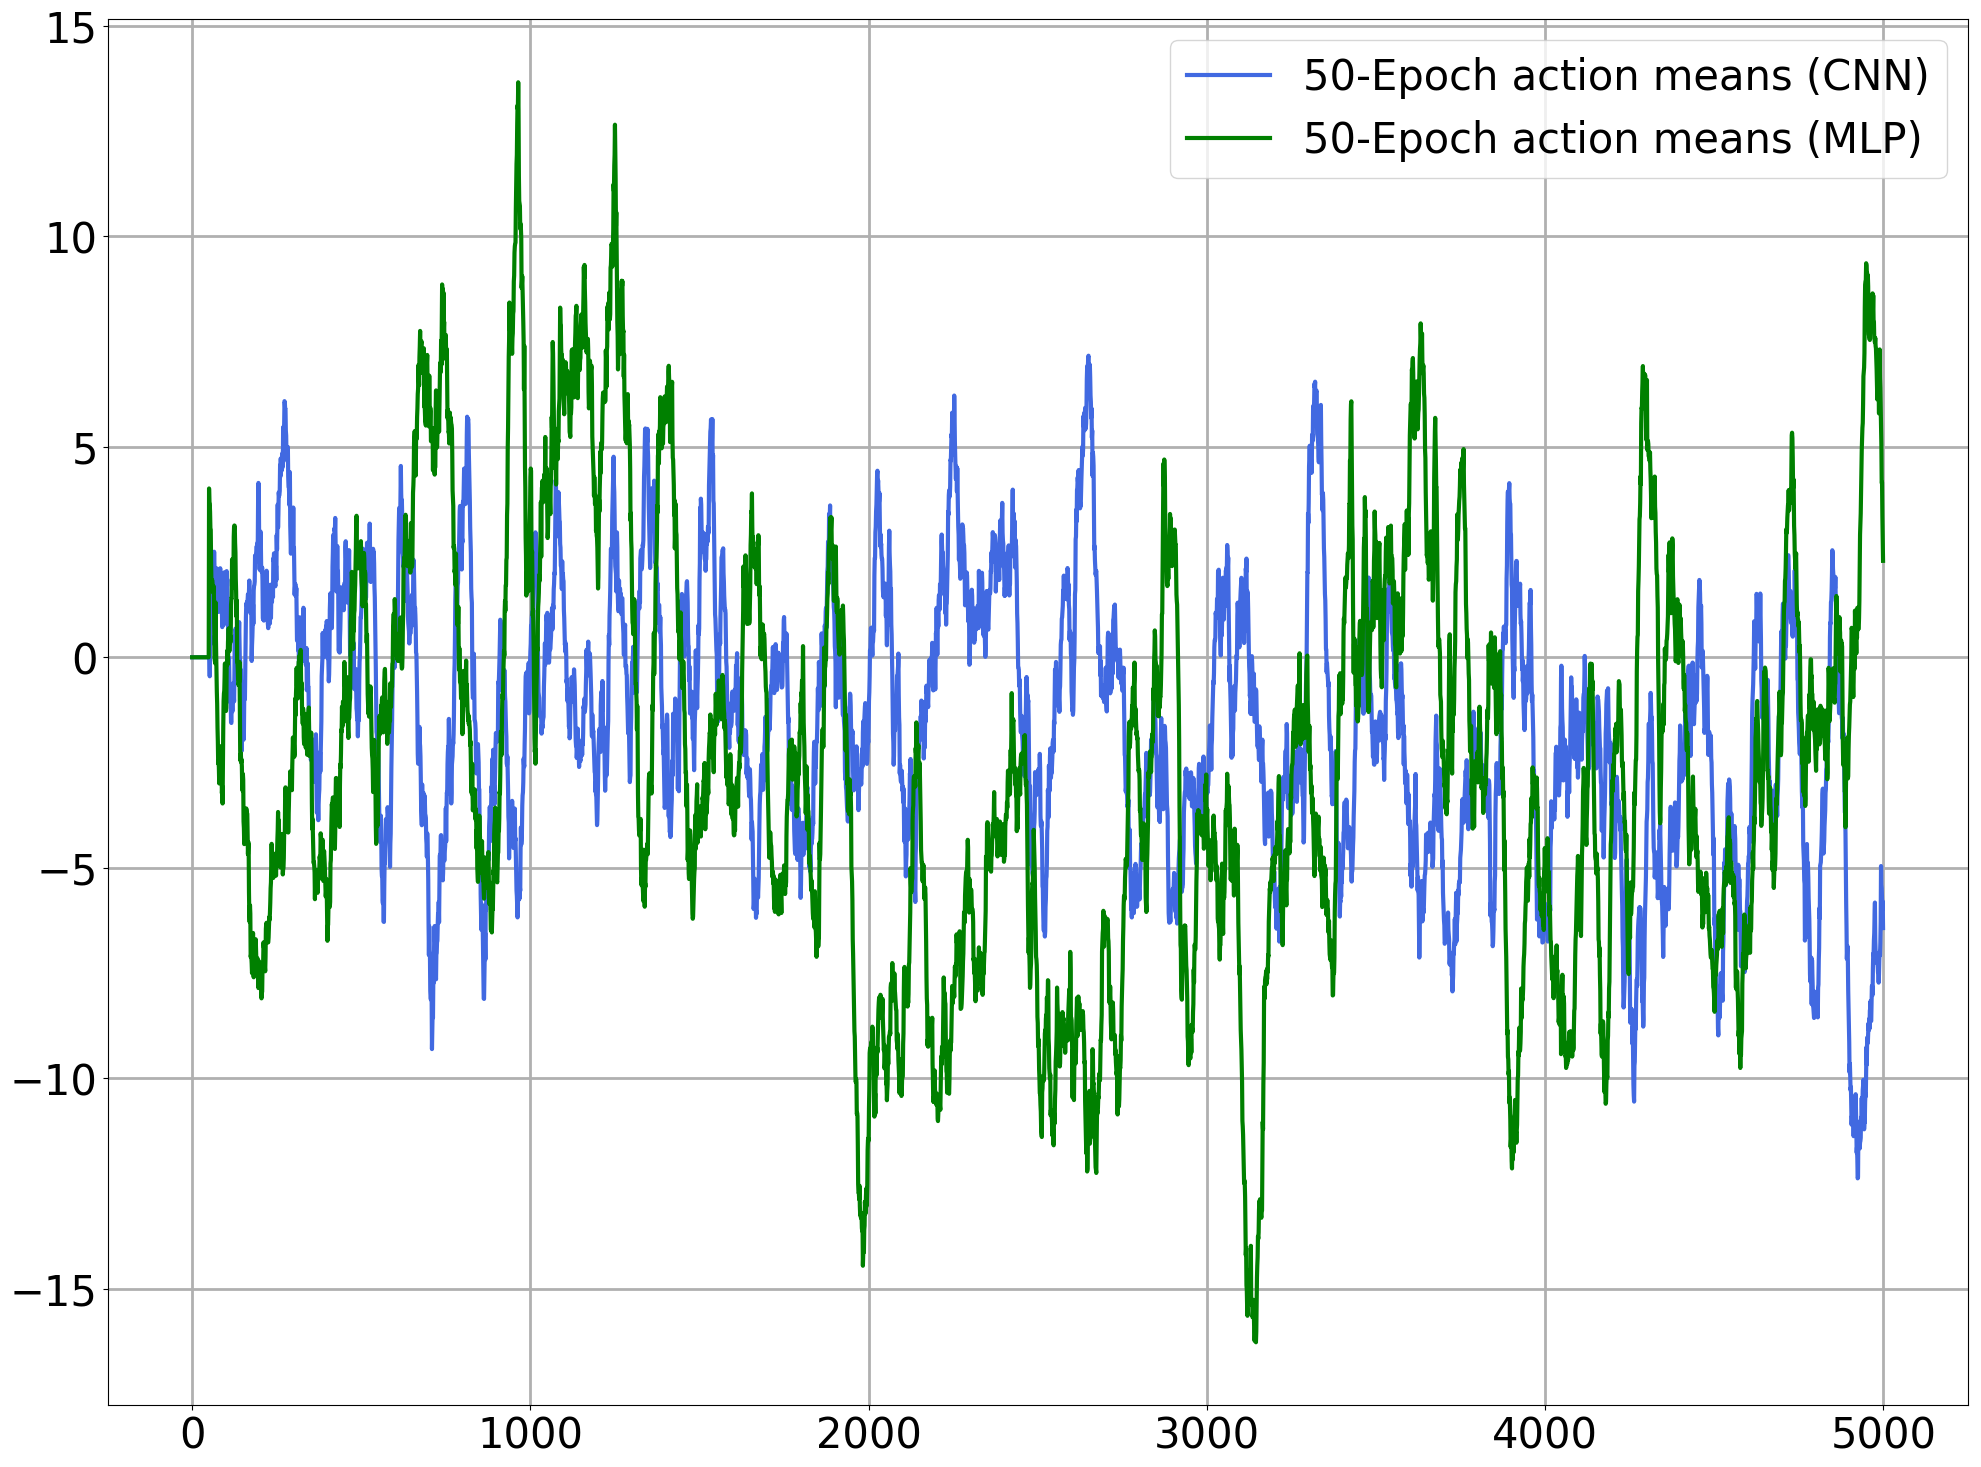
\includegraphics[width=\textwidth]{cnn_nn_1_sell_bidask_mean_actions.png}
        \caption{Mean of actions per epoch (sell)}
        \label{fig:analysis-dqn-1-action-sell}
    \end{subfigure}
    \caption{DQN agent rewards and mean of actions for buying and selling on training data set I using feature I.}
    \label{fig:analysis-dqn-1}
\end{figure}

\begin{figure}[H]
    \centering
    \begin{subfigure}[b]{0.4\textwidth}
        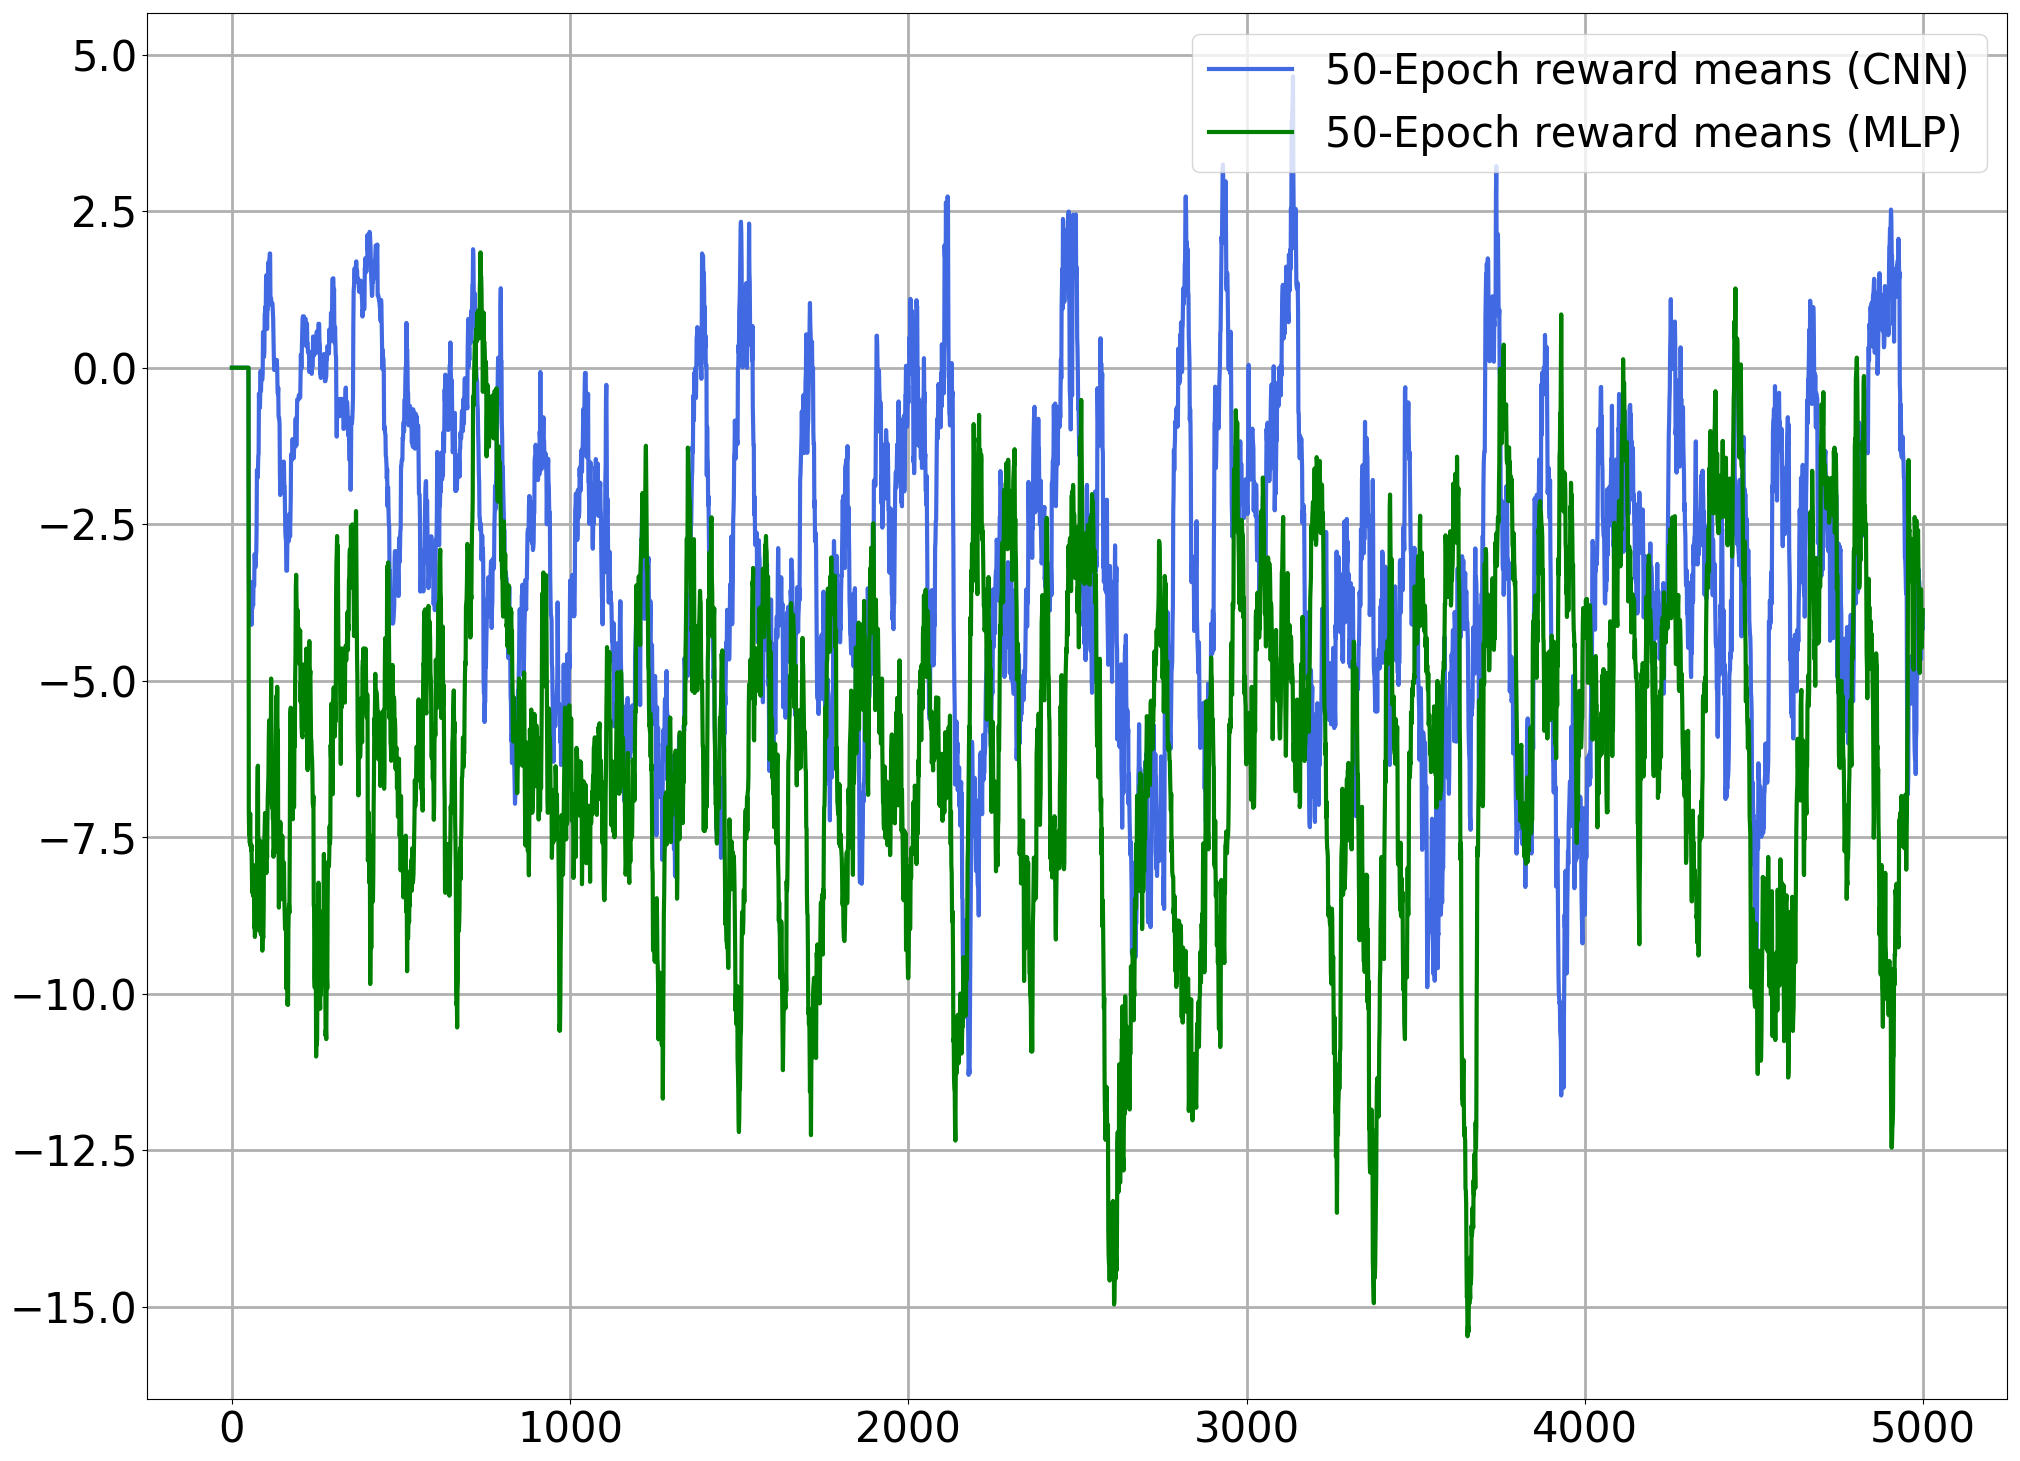
\includegraphics[width=\textwidth]{cnn_nn_2_buy_bidask_rewards.png}
        \caption{Reward per epoch (buy)}
        \label{fig:analysis-dqn-2-reward-buy}
    \end{subfigure}
    \begin{subfigure}[b]{0.4\textwidth}
        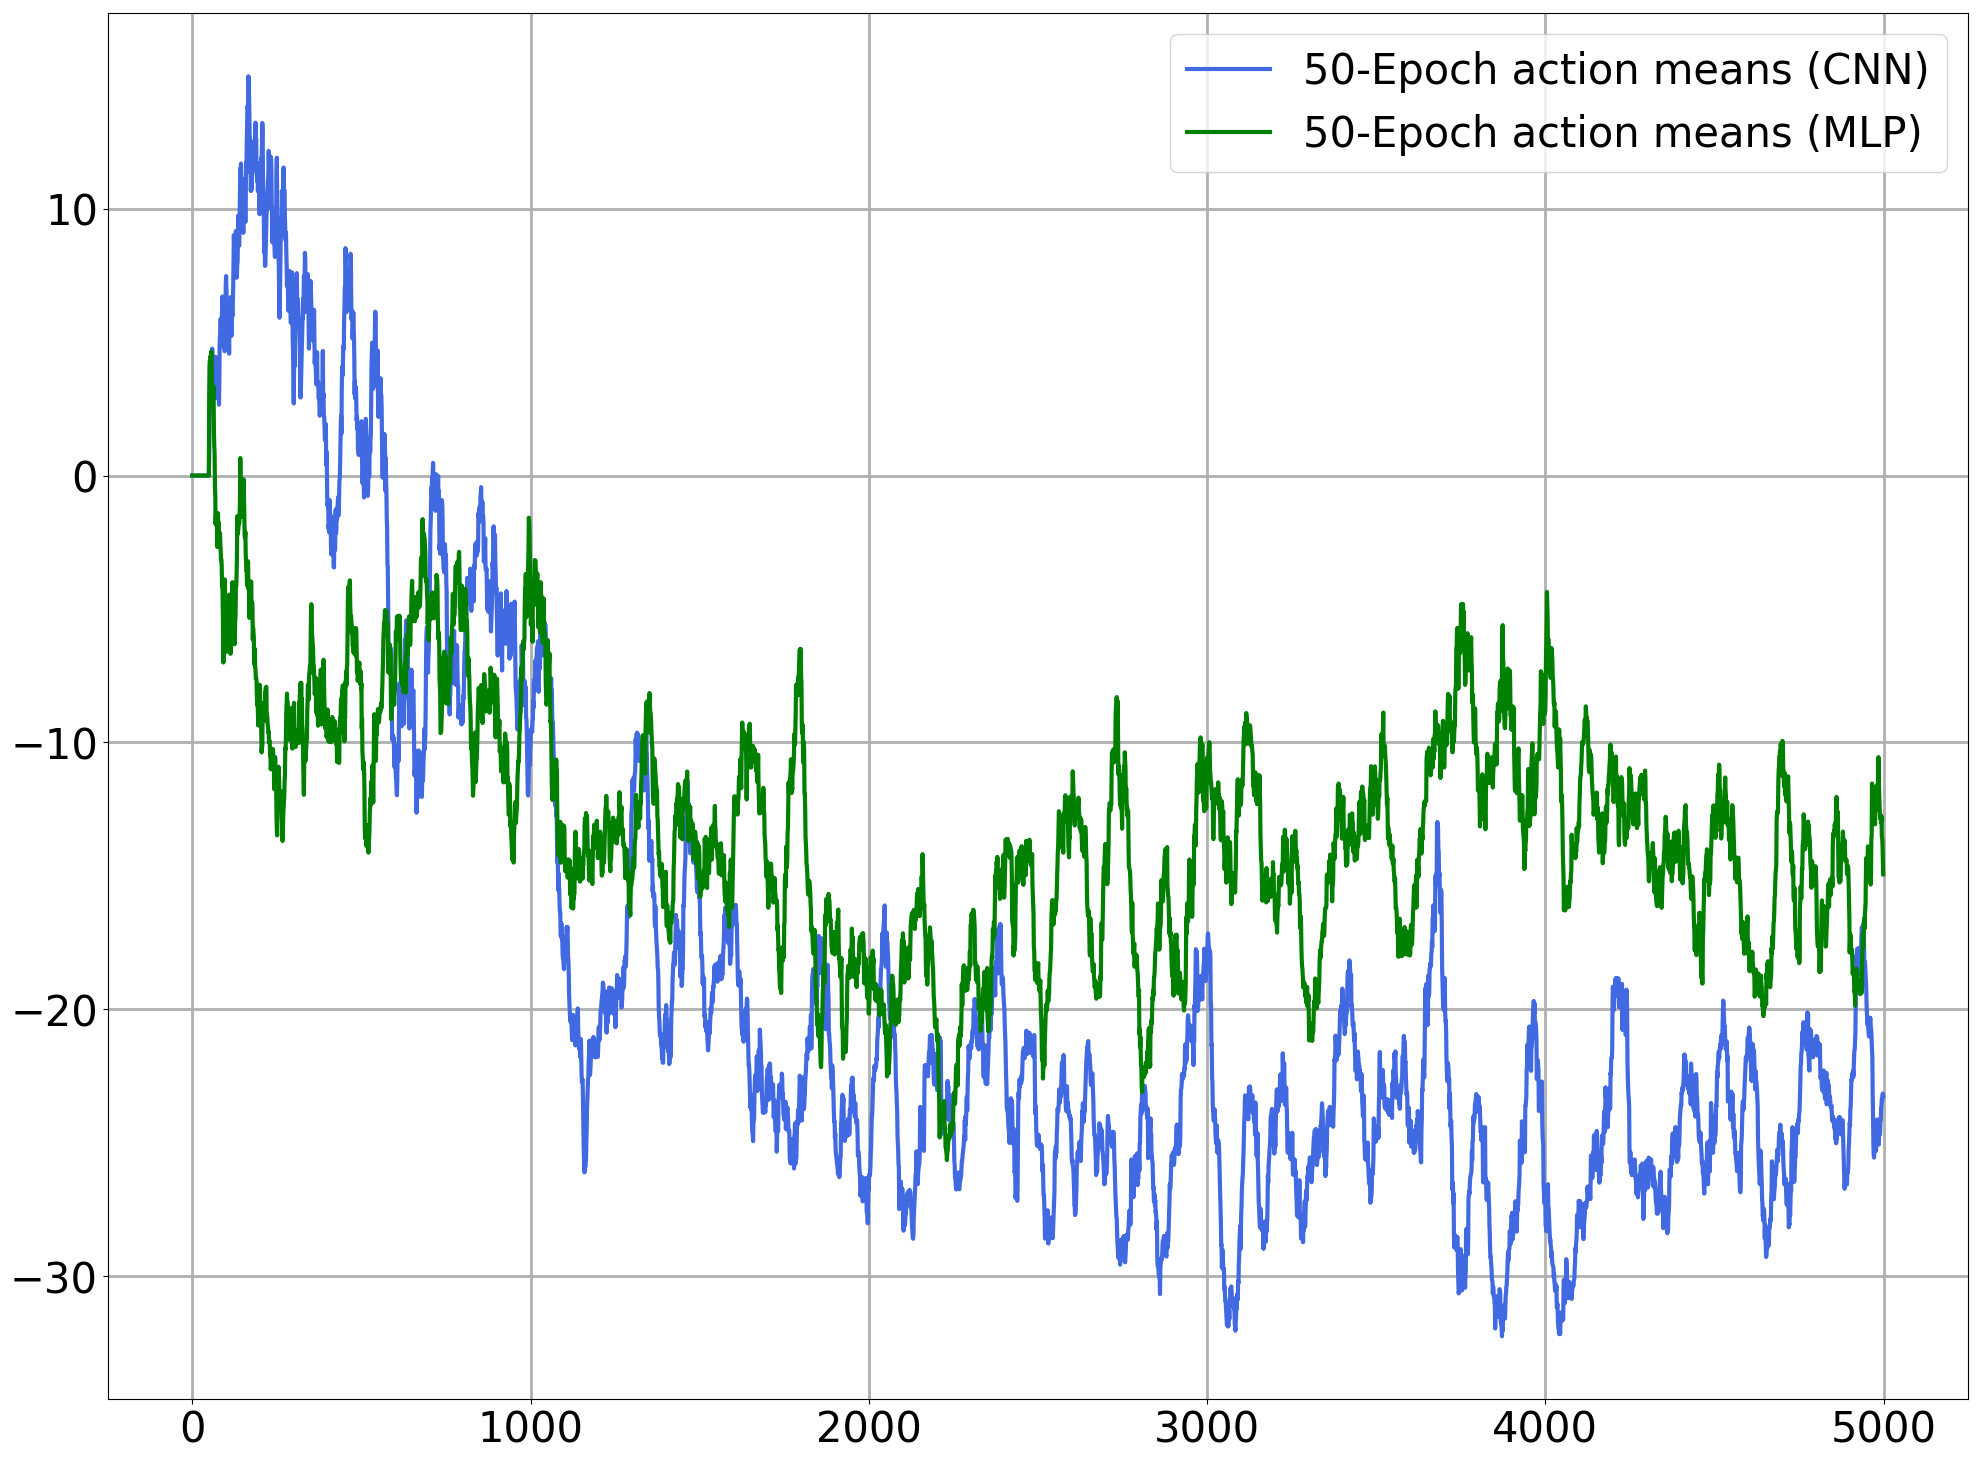
\includegraphics[width=\textwidth]{cnn_nn_2_buy_bidask_mean_actions.png}
        \caption{Mean of actions per epoch (buy)}
        \label{fig:analysis-dqn-2-action-buy}
    \end{subfigure}
    \begin{subfigure}[b]{0.4\textwidth}
        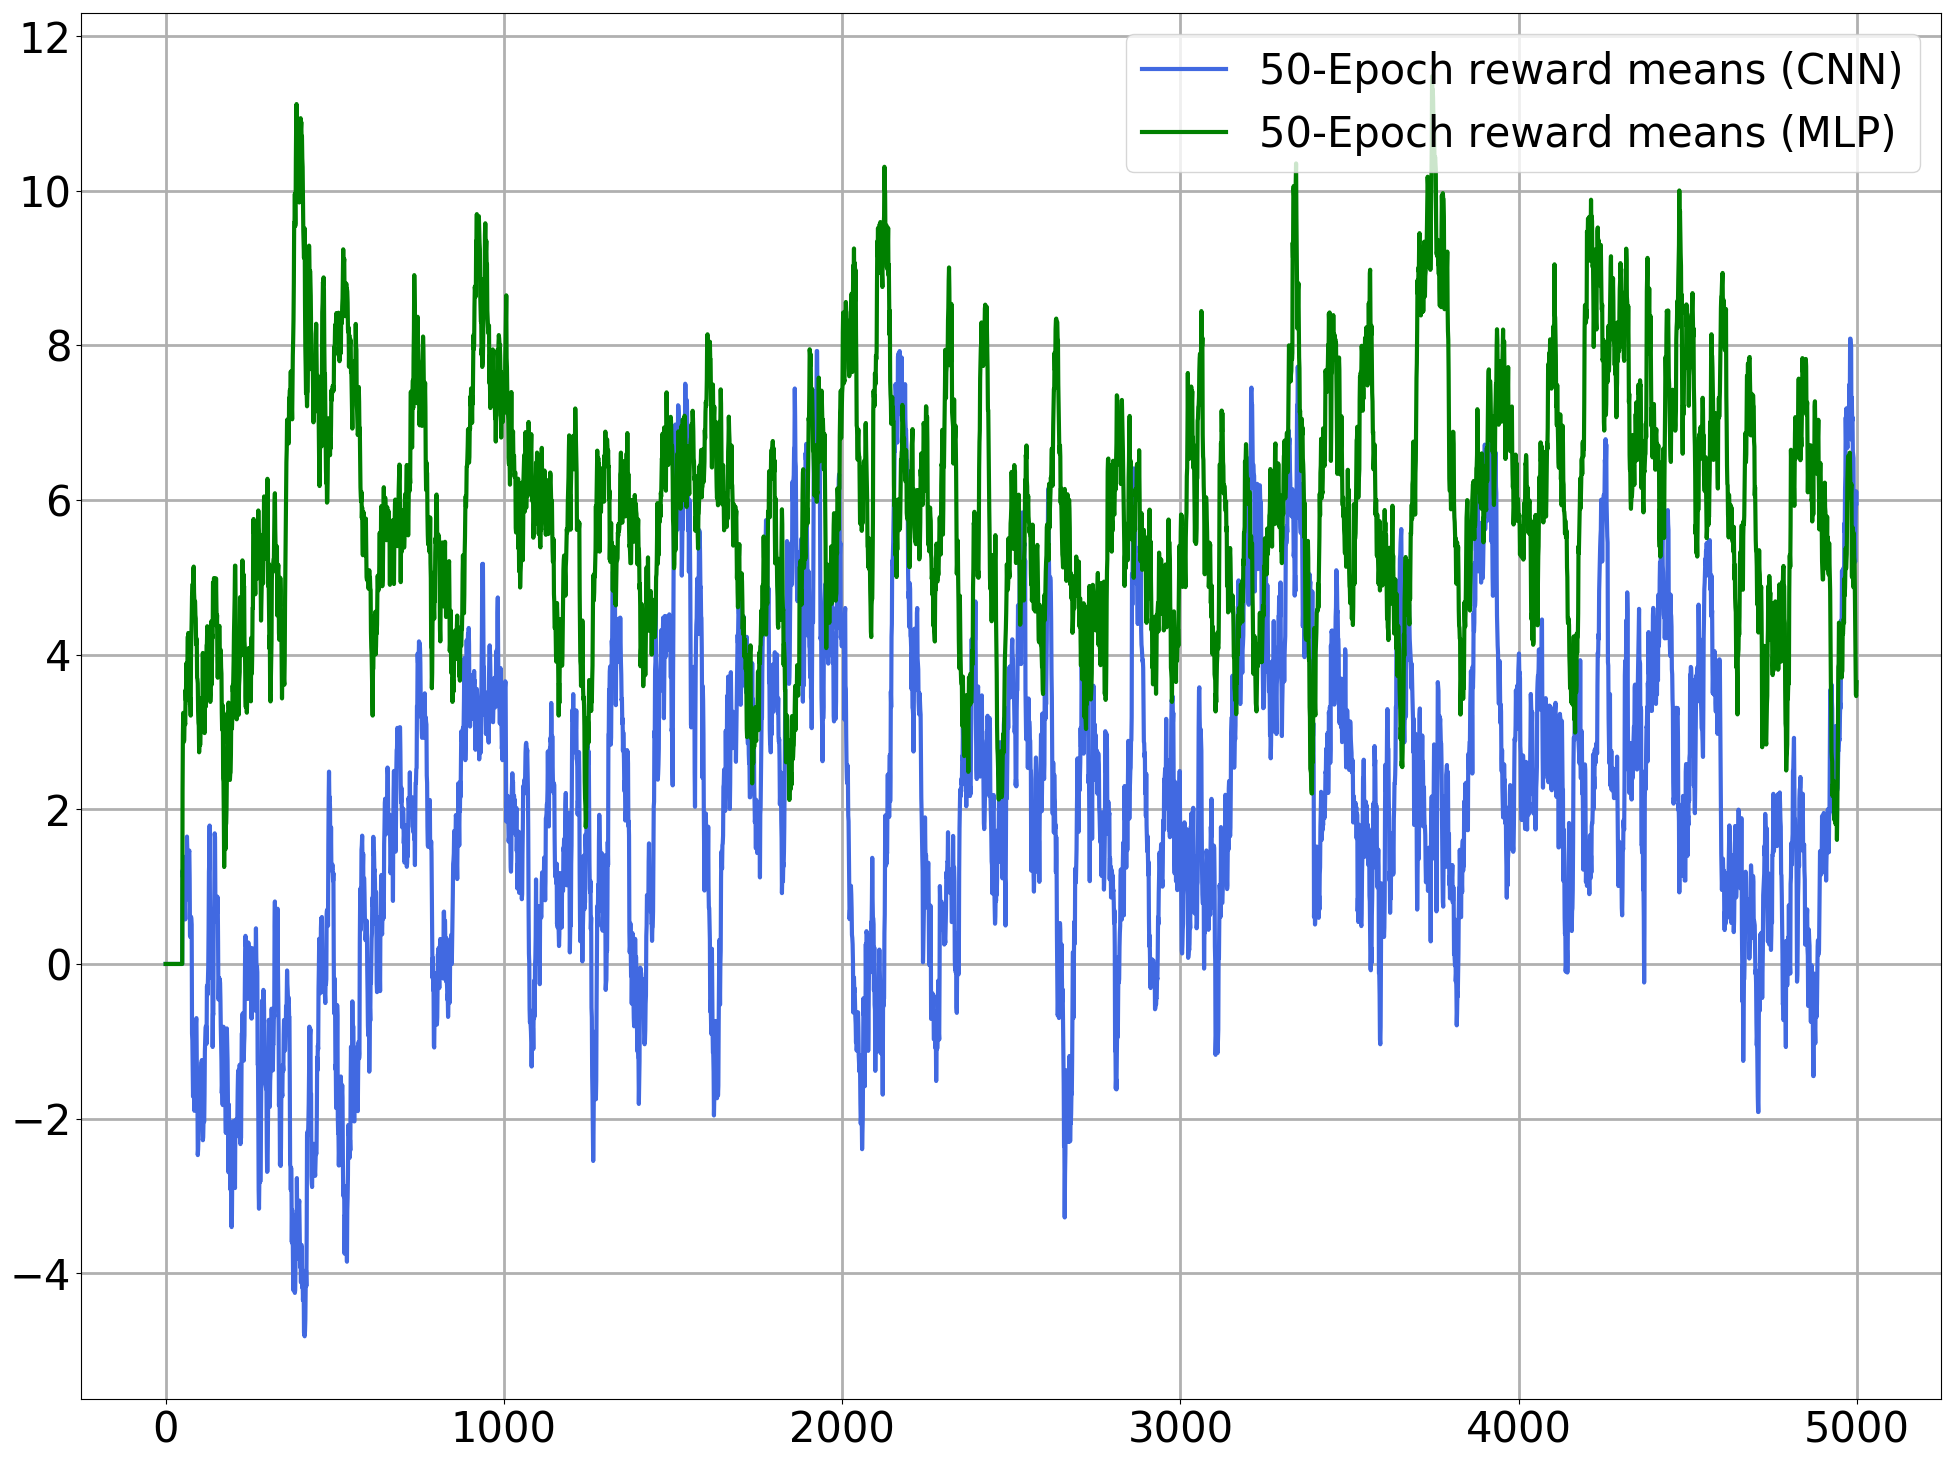
\includegraphics[width=\textwidth]{cnn_nn_2_sell_bidask_rewards.png}
        \caption{Mean rewards per epoch (sell)}
        \label{fig:analysis-dqn-2-reward-sell}
    \end{subfigure}
    \begin{subfigure}[b]{0.4\textwidth}
        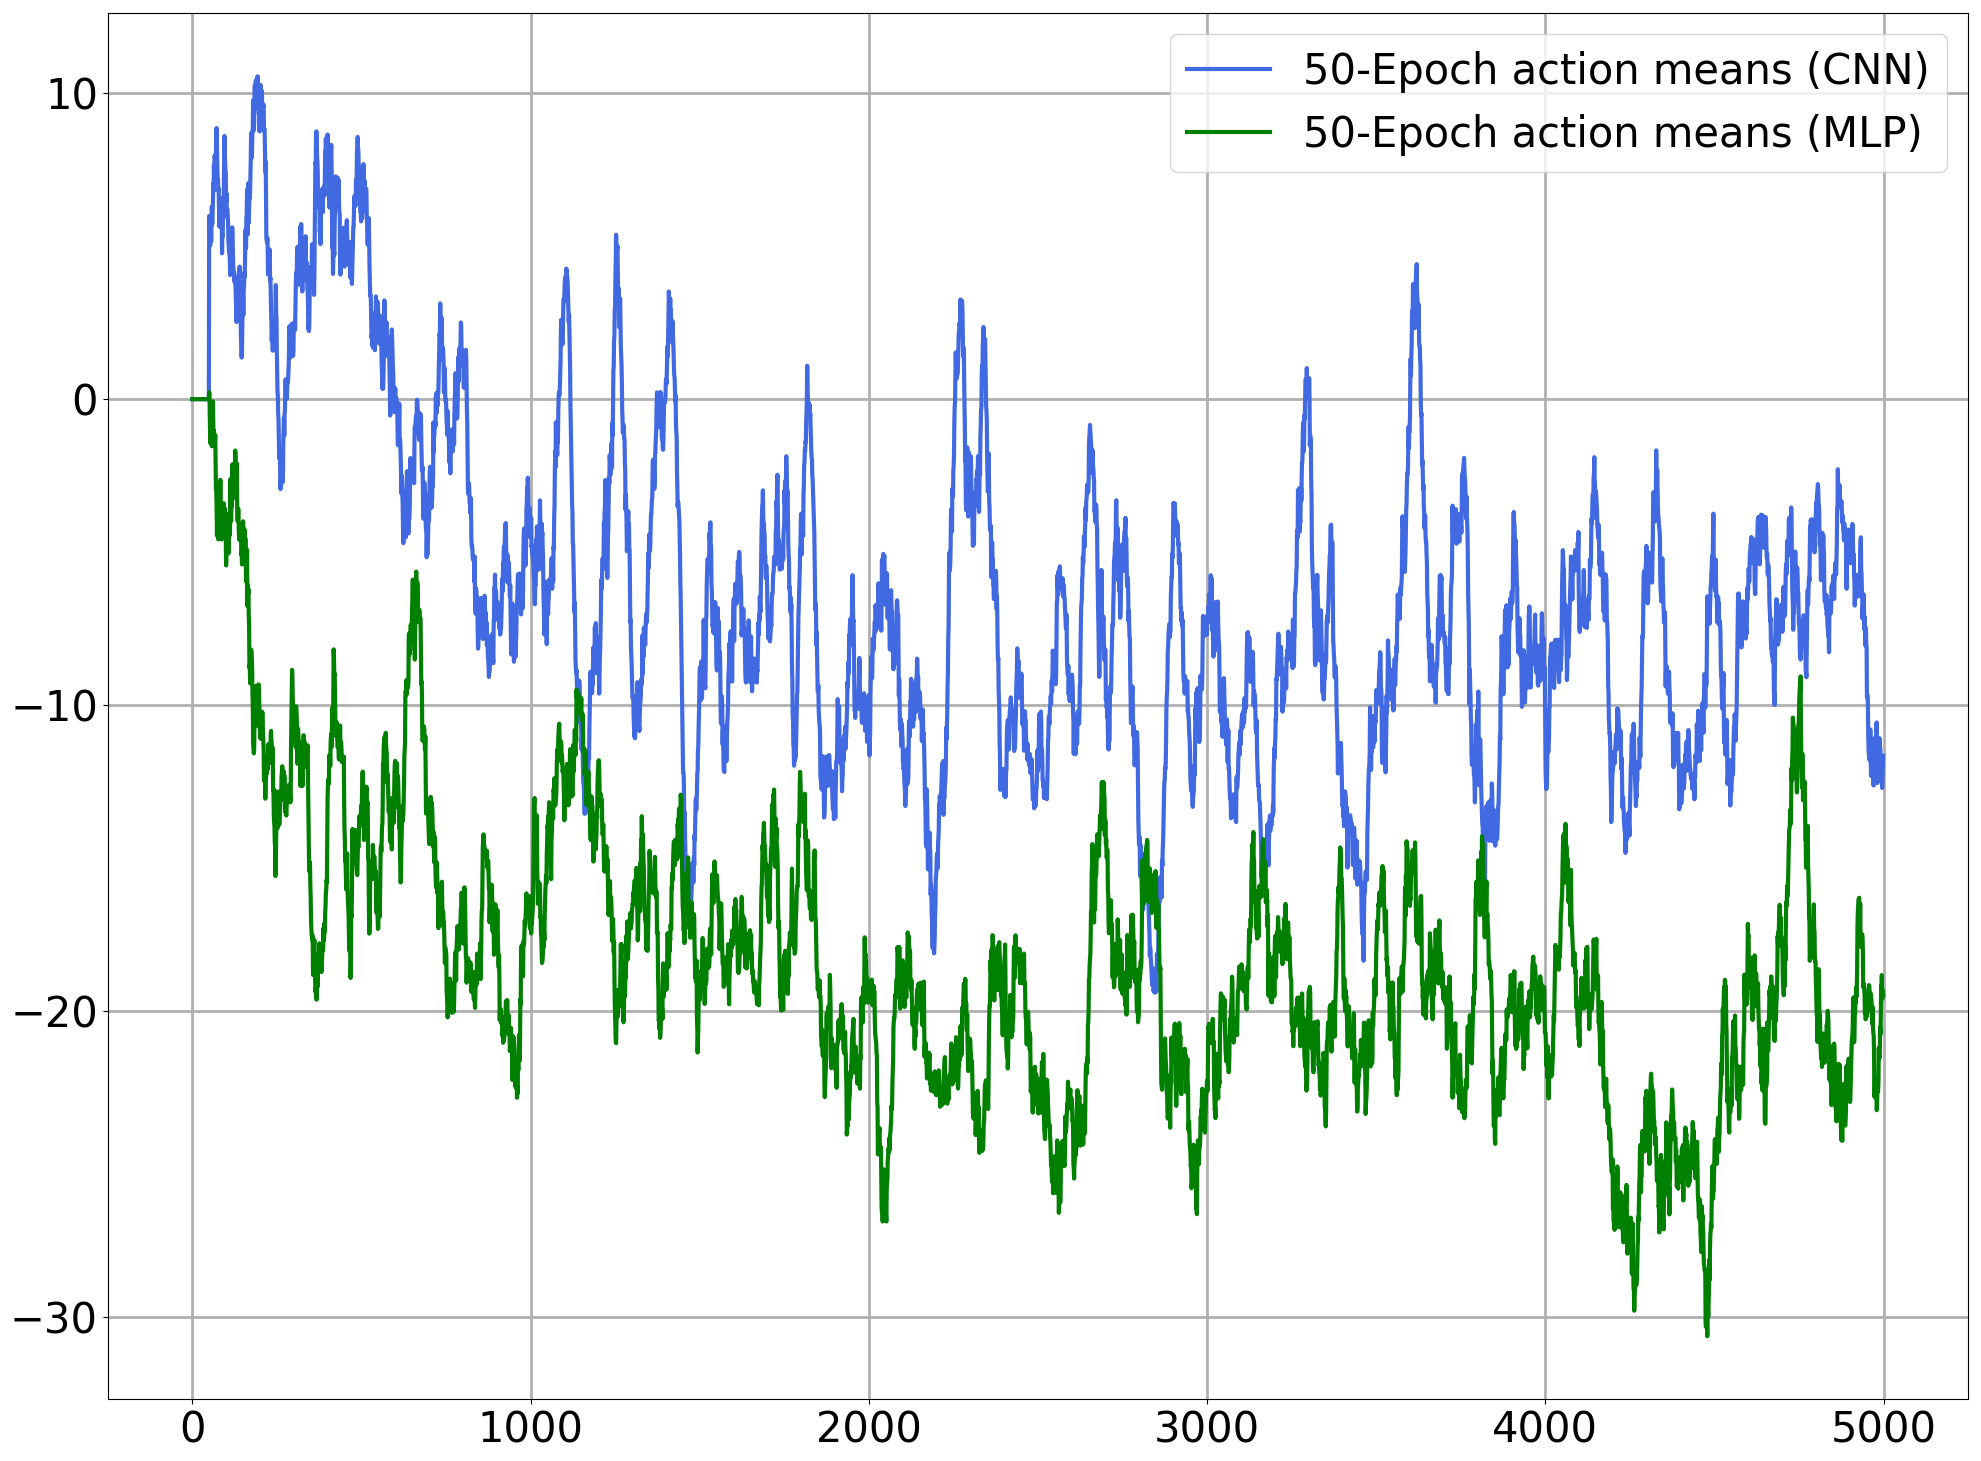
\includegraphics[width=\textwidth]{cnn_nn_2_sell_bidask_mean_actions.png}
        \caption{Mean of actions per epoch (sell)}
        \label{fig:analysis-dqn-2-action-sell}
    \end{subfigure}
    \caption{DQN agent rewards and mean of actions for buying and selling on training data set II using feature I.}
    \label{fig:analysis-dqn-2}
\end{figure}

Figure \ref{fig:analysis-dqn-1} shows the learning process using data set I.
During the training process relating to the purchase of assets, the rewards obtained consistently improved over the course of the 5000 epochs (Figure \ref{fig:analysis-dqn-1-reward-buy}), throughout which the DQN-CNN agent steadily adjusted its actions to be more negative and the DQN-MLP agent adjusted them to become more positive (Figure \ref{fig:analysis-dqn-1-action-buy}).
It is evident that this adjustment, for both DQN agents, is not as linear as it was during the training of the Q-Learning agent, as shown in the previous section.
However, the adjustment made by the DQN-CNN agent is appropriate since the market price was falling.
The rewards obtained from selling are shown in Figure \ref{fig:analysis-dqn-1-reward-sell} and the average chosen action throughout the epochs is shown in Figure \ref{fig:analysis-dqn-1-action-sell}.
The rewards did not improve over the course of the training and both agents did not choose to adjust the average actions.
Possibly, this was due to the constantly negative rewards obtained during the training under market conditions that were difficult for the sale of assets while the market price was falling.
Figure \ref{fig:analysis-dqn-2} shows the agents learning processes using data set II.
Over the course of 5000 epochs, the agents were not able to improve their reward and instead, stagnated at approximately \$-2.50 and \$5.00 rewards per epoch respectively, as shown in Figure \ref{fig:analysis-dqn-2-reward-buy}.
Both agents adjusted the actions steadily such that the average limit level fell to approximately -20 at epoch 1000 and remained at this level, as shown in Figure \ref{fig:analysis-dqn-2-action-buy}.
Therefore, the rewards must have been determined by market orders followed after those which failed to fill the order with their levels chosen.
The rewards for the agent that learned to sell assets are shown in Figure \ref{fig:analysis-q-learn-2-reward-sell}.
The rewards could not be improved during the training, even though the agent lowered the average action chosen to below -20, as shown in Figure \ref{fig:analysis-q-learn-2-action-sell}.
In such rising market conditions, the rewards observed are a product of the market order, since negative actions will likely not result in a filled order.
The rewards for selling assets in this rising market was improved and remained above \$0.00, as shown in Figure \ref{fig:analysis-q-learn-2-reward-sell}.
Thereby, the average of the actions chosen for an epoch reduced within the first 1000 epochs and, thereafter, remained at approximately -10 (DQN-CNN) and -20 (DQN-MLP), which correlates with the rewards obtained .
\\
\\
Table \ref{tbl:analysis-dqn-orderfeature-summary} summarizes the average rewards observed during the backtest using the DQN agents that made use of Feature I.
Overall, both DQN agents were able to optimize limit order placement when the given market conditions became favorable to making a purchase or sale respectively.
More precisely, significant improvements were made during the backtest of the DQN-CNN agent when the task was to buy assets and the market price was falling (data set I). 
Thereby, the agent was rewarded with 22.06, which is a significant improvement compared to the expected return of -0.05 for a market order.
Likewise, during rising market conditions (data set I), both agents were able to improve by more than the expected market order return.
However, when market conditions were not favorable to an intention to either buy or sell, the agents mostly performed not only worse than the expected return of a market order but also worse than the Q-Learning agent (see Table \ref{tbl:analysis-q-learn-summary} above).
That is, the DQN-CNN agent achieved rewards of -39.26 and -2.26 when selling in data set I and buying in data set II, which were both worse than the expected returns for market orders.
The exception was when the DQN-MLP agent achieved -22.67 when attempting to make sales in data set I and therefore, it performed better than the expected market order return.
However, the backtest that set the DQN-MLP agent to make purchases in data set II performed, with -7.40, much worse than the baseline provided by the expected market order return.
Overall, the DQN-CNN agent performed the best and minor improvements were achieved by the DQN-MLP agent.

\begin{table}[H]
\centering
\begin{tabular}{l|l|l|l|}
\cline{2-4}
& \textbf{DQN-CNN} & \textbf{DQN-MLP} & \textbf{\begin{tabular}[c]{@{}l@{}}$\mathbb{E}$[Market\\ Order]\end{tabular}} \\ \hline
\multicolumn{1}{|l|}{\textbf{Buy (I)}}   & 22.06  & -4.04 & -0.05                                                           \\ \hline
\multicolumn{1}{|l|}{\textbf{Sell (I)}}  & -39.26 & -22.67        & -27.70                                                          \\ \hline
\multicolumn{1}{|l|}{\textbf{Buy (II)}}  & -2.26  & -7.40        & -1.06                                                           \\ \hline
\multicolumn{1}{|l|}{\textbf{Sell (II)}} & 0.84   & 7.47       & -1.72                                                           \\ \hline
\multicolumn{1}{|l|}{\textbf{$\Sigma$}} & -18.62  & -26.64        & -30.53                                                           \\ \hline
\end{tabular}
\caption{Summary of rewards during backtest of DQN agent using Feature I (historical orders).}
\label{tbl:analysis-dqn-orderfeature-summary}
\end{table}

\subsection{Application of historical trade feature}

The following evaluation of the DQN agent setups that consider Feature II, as described in Chapter \ref{chap:data} (Section \ref{sec:data-feature-2}).
In this initial run we consider $n=30$ historical trades.
This results in a feature set size of $(30, 3)$, as a consequence of the defined size $(n, 4)$.
When we included the two private variables by appending a vector $[inventory, time, 0, 0]$ at the beginning of this feature vector, the size of the feature set was $(31, 4)$ and, as such, will serve as the input for the neural networks in use.

\begin{figure}[H]
    \centering
    \begin{subfigure}[b]{0.4\textwidth}
        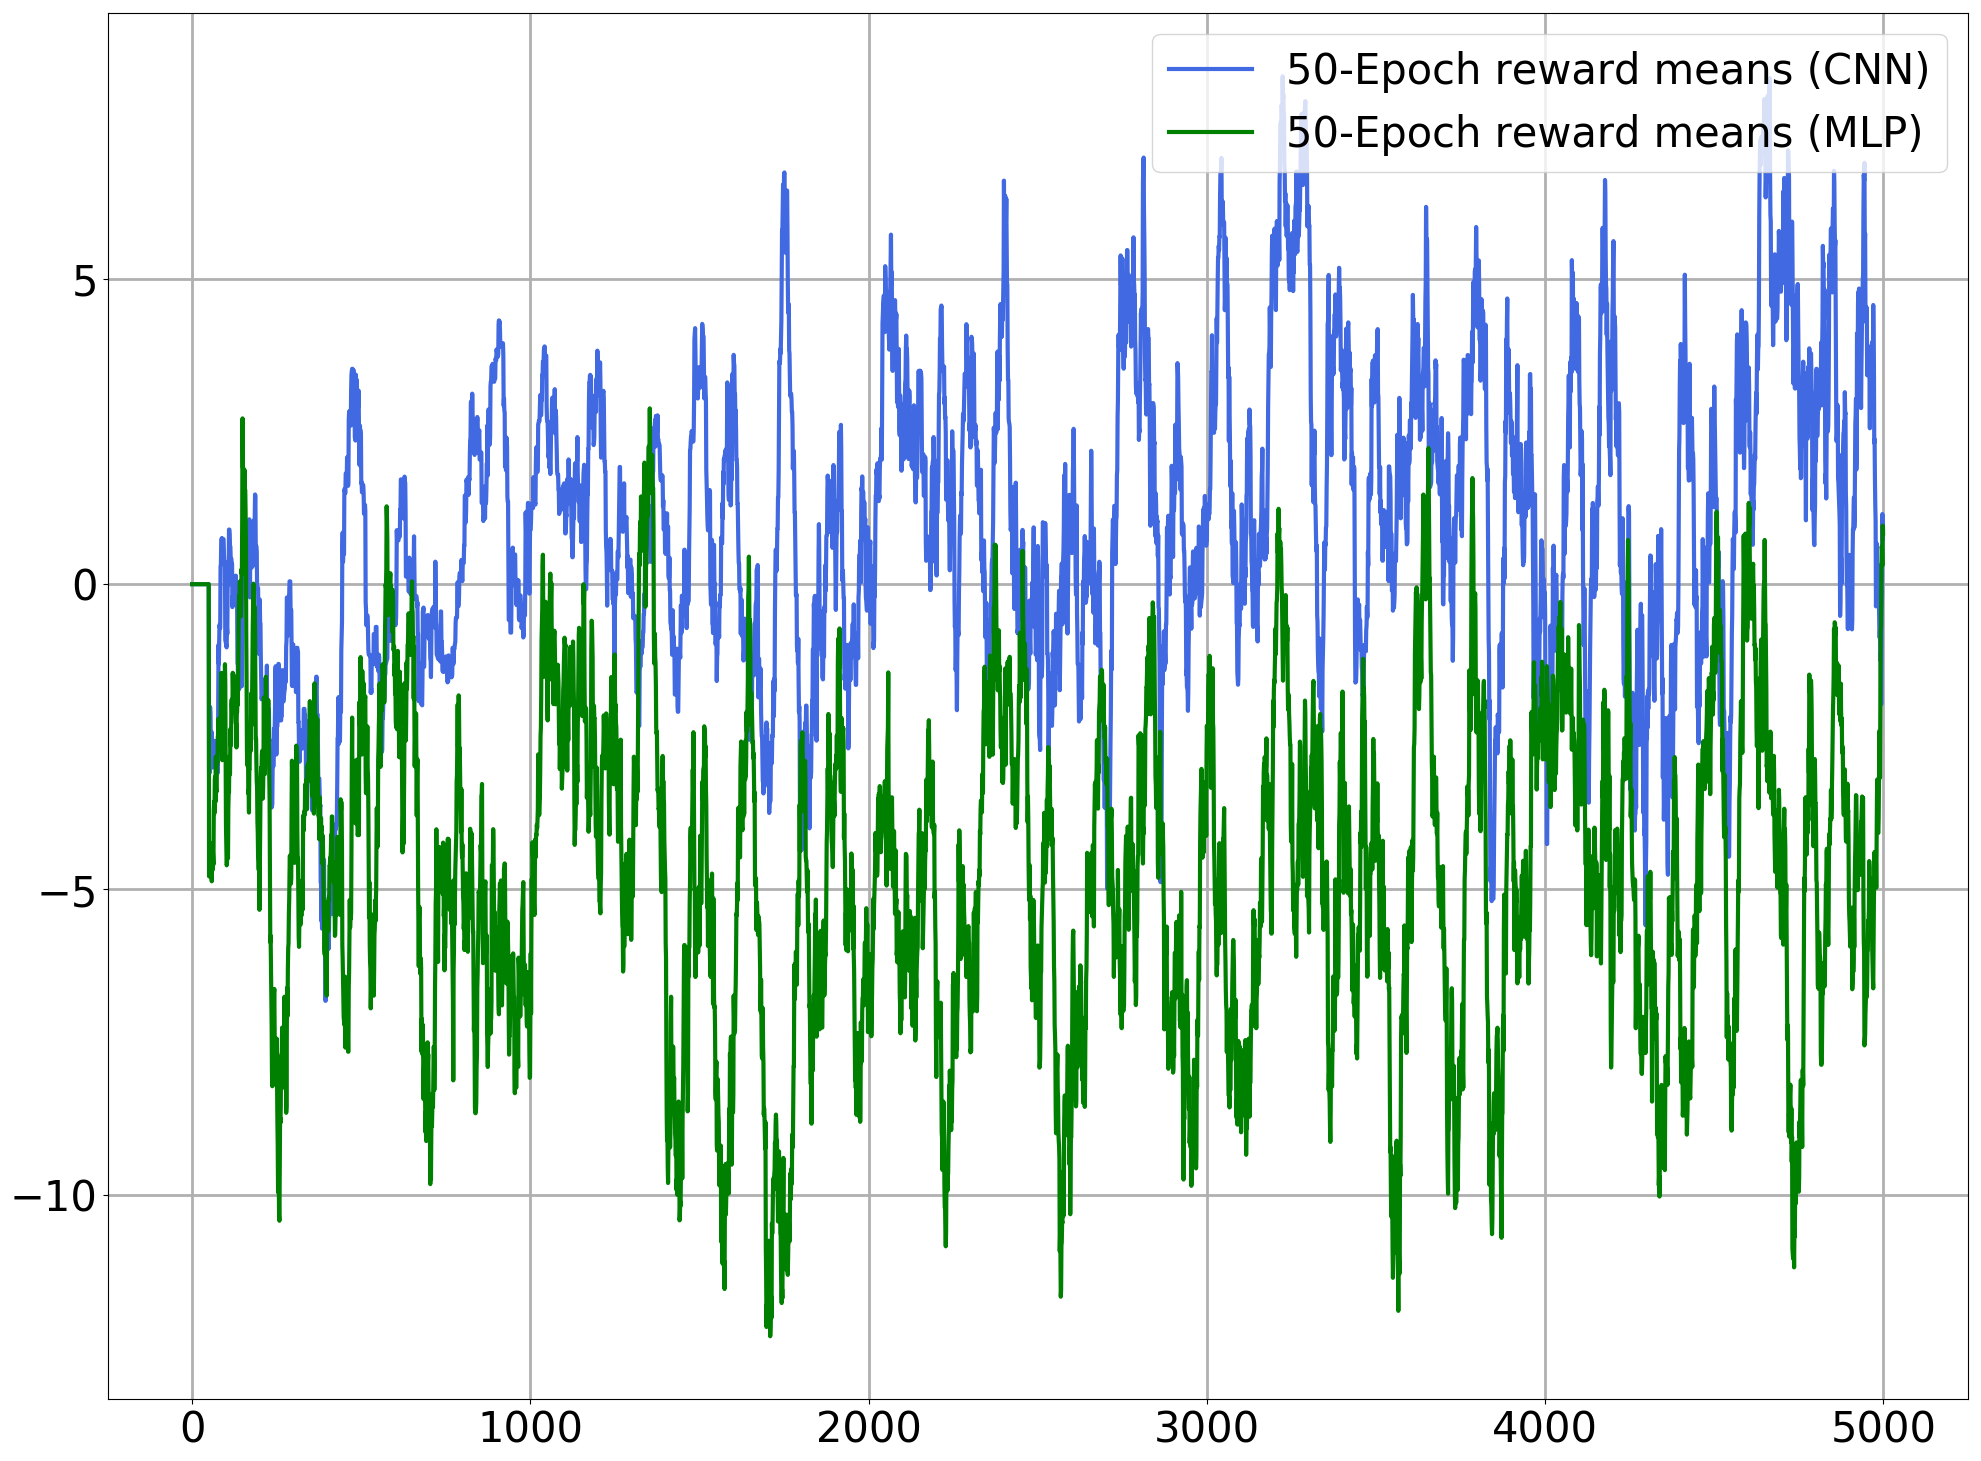
\includegraphics[width=\textwidth]{cnn_nn_1_buy_trades_rewards.png}
        \caption{Reward per epoch (buy)}
        \label{fig:analysis-dqn-1-trades-reward-buy}
    \end{subfigure}
    \begin{subfigure}[b]{0.4\textwidth}
        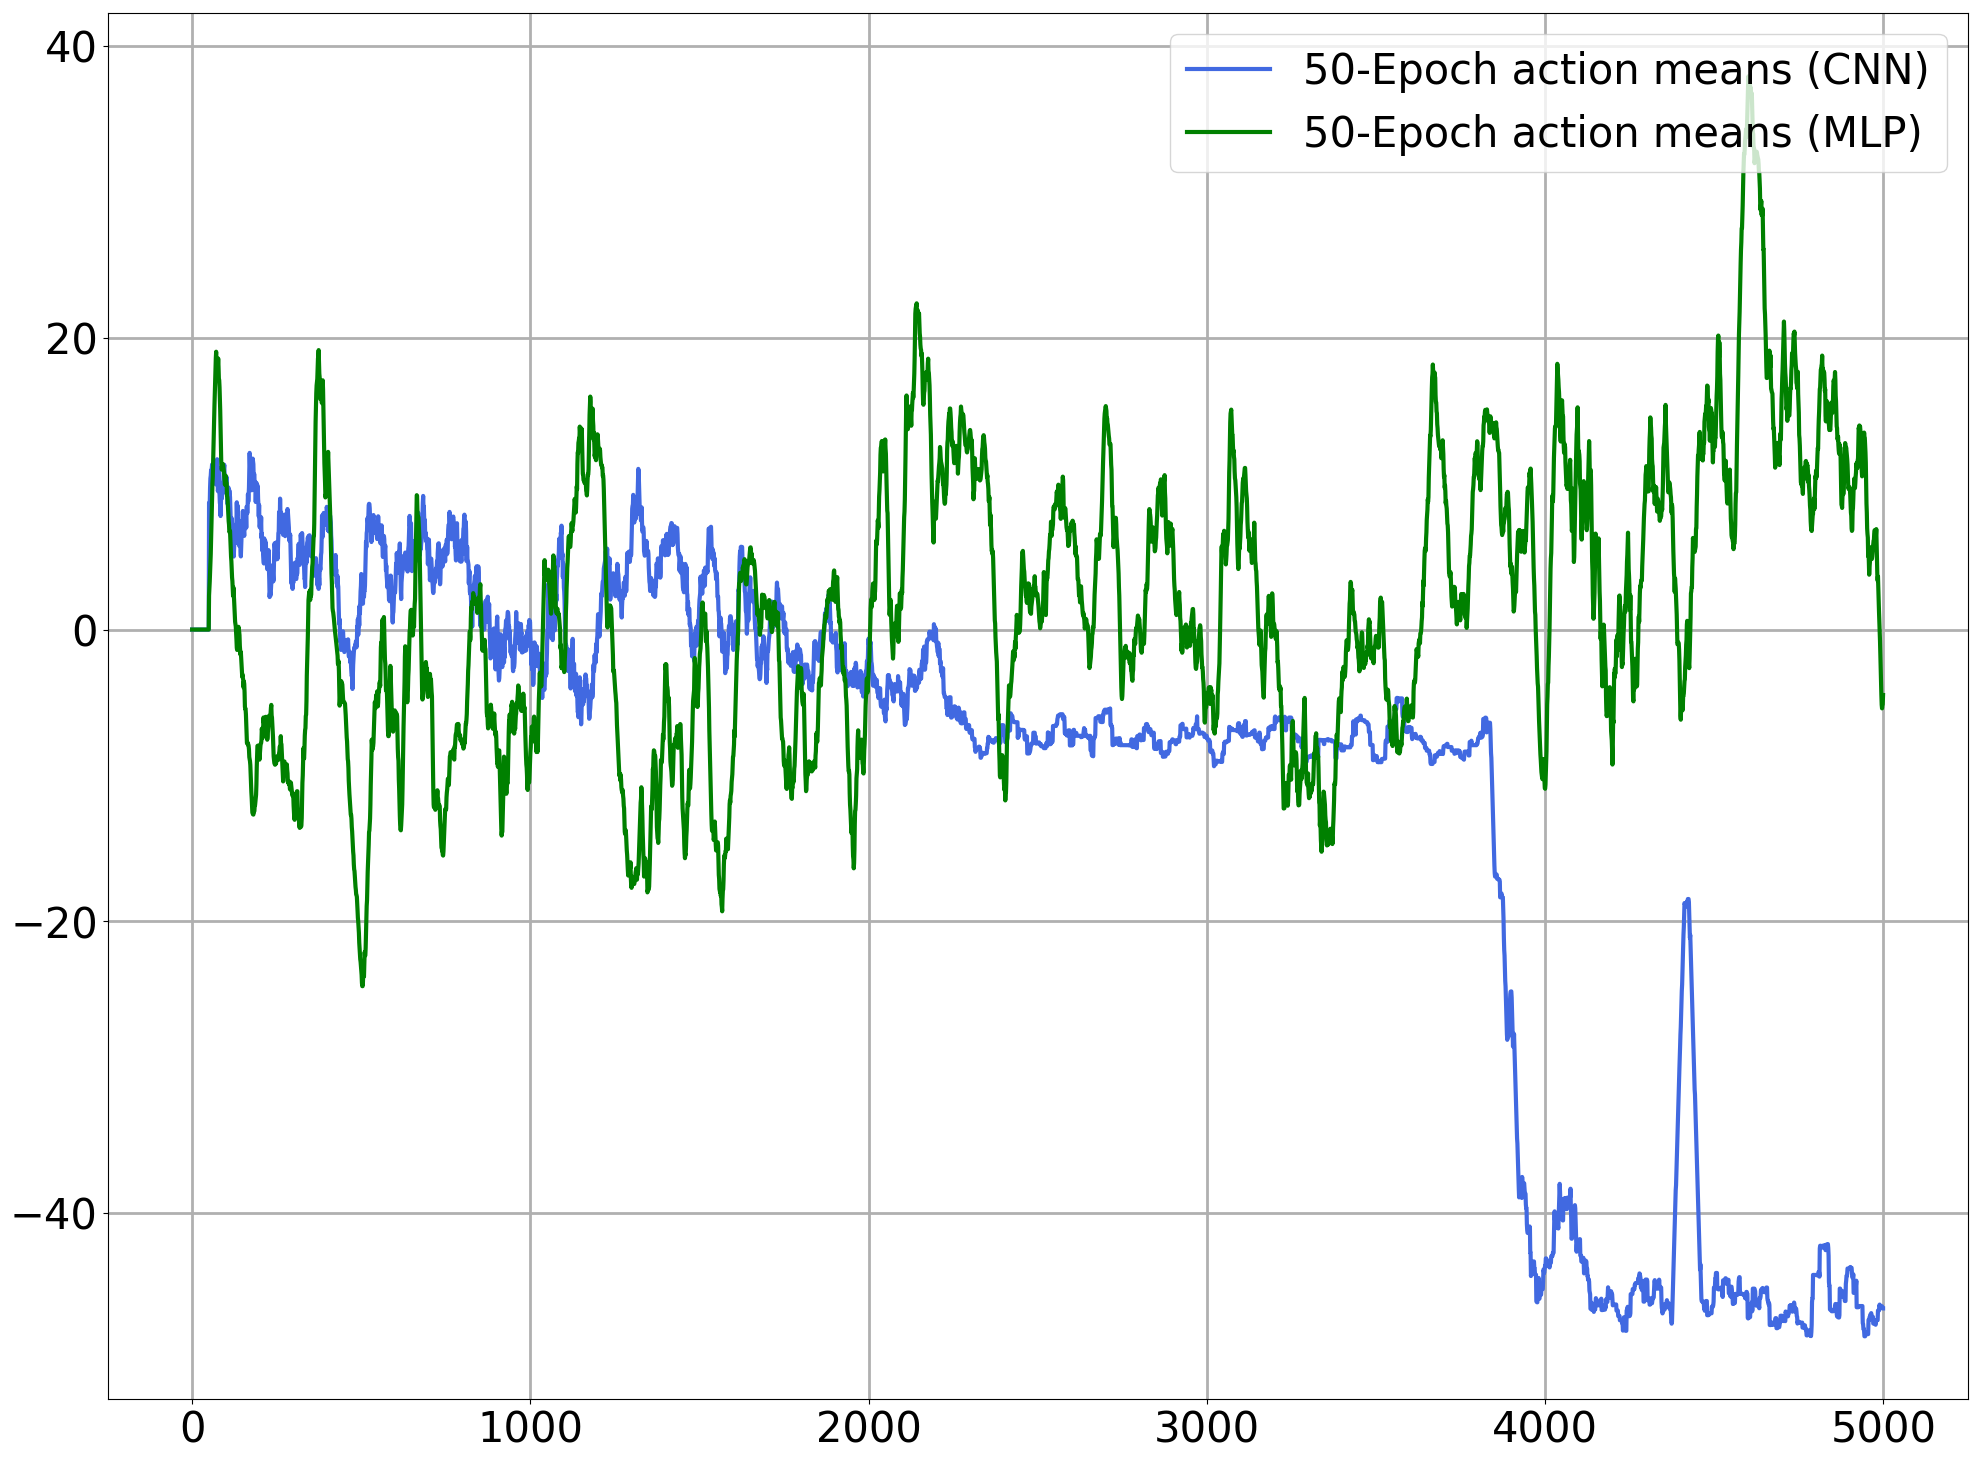
\includegraphics[width=\textwidth]{cnn_nn_1_buy_trades_mean_actions.png}
        \caption{Mean of actions per epoch (buy)}
        \label{fig:analysis-dqn-1-trades-action-buy}
    \end{subfigure}
    \begin{subfigure}[b]{0.4\textwidth}
        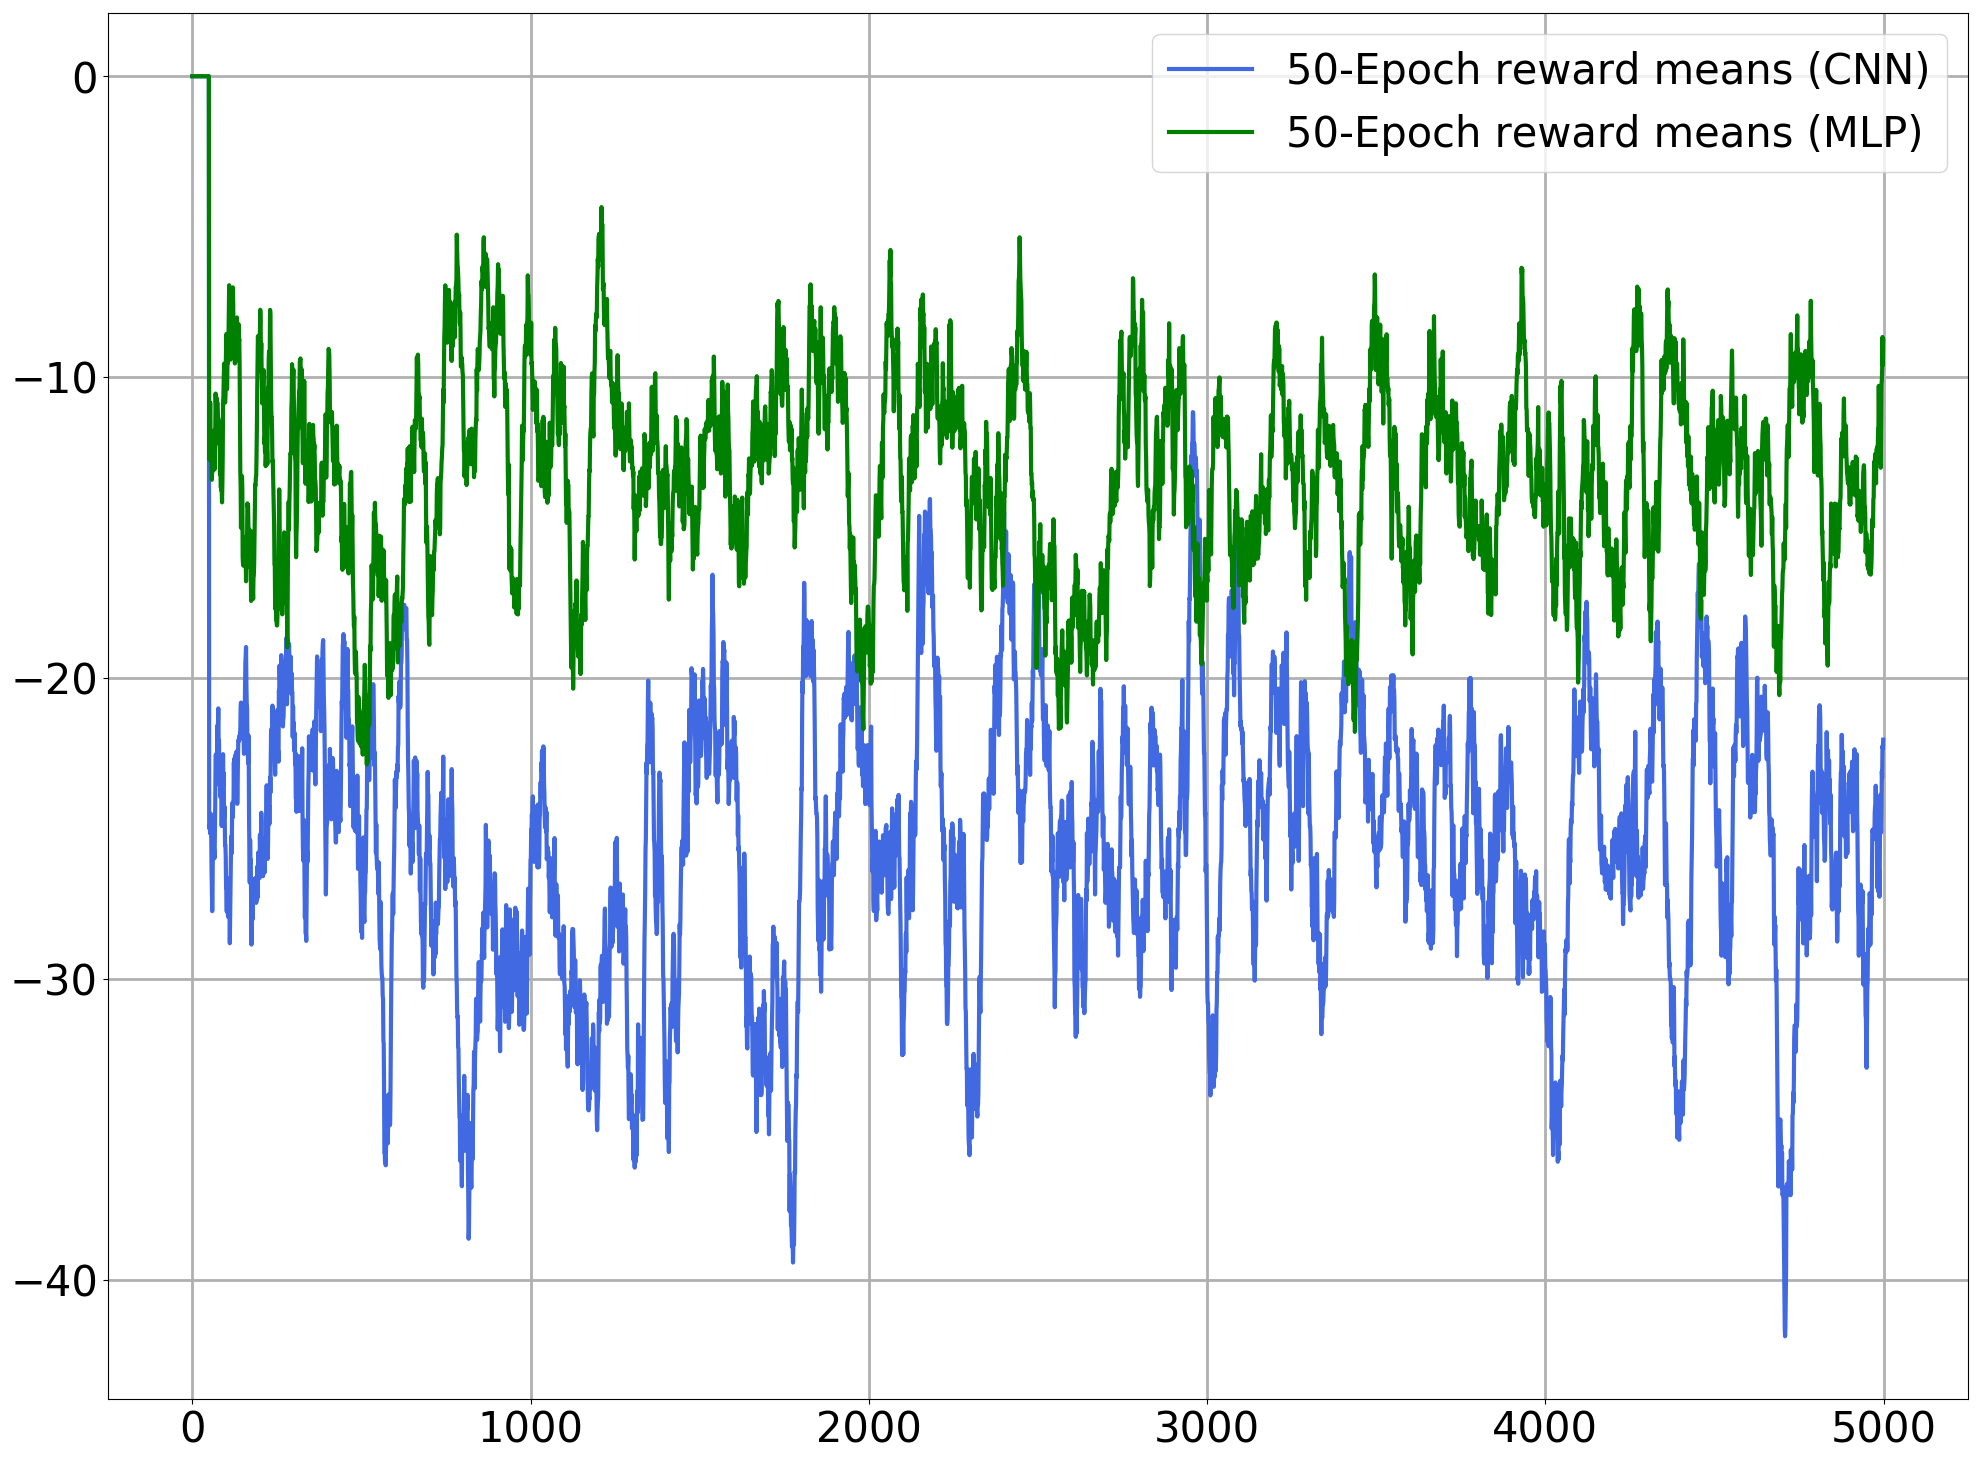
\includegraphics[width=\textwidth]{cnn_nn_1_sell_trades_rewards.png}
        \caption{Mean rewards per epoch (sell)}
        \label{fig:analysis-dqn-1-trades-reward-sell}
    \end{subfigure}
    \begin{subfigure}[b]{0.4\textwidth}
        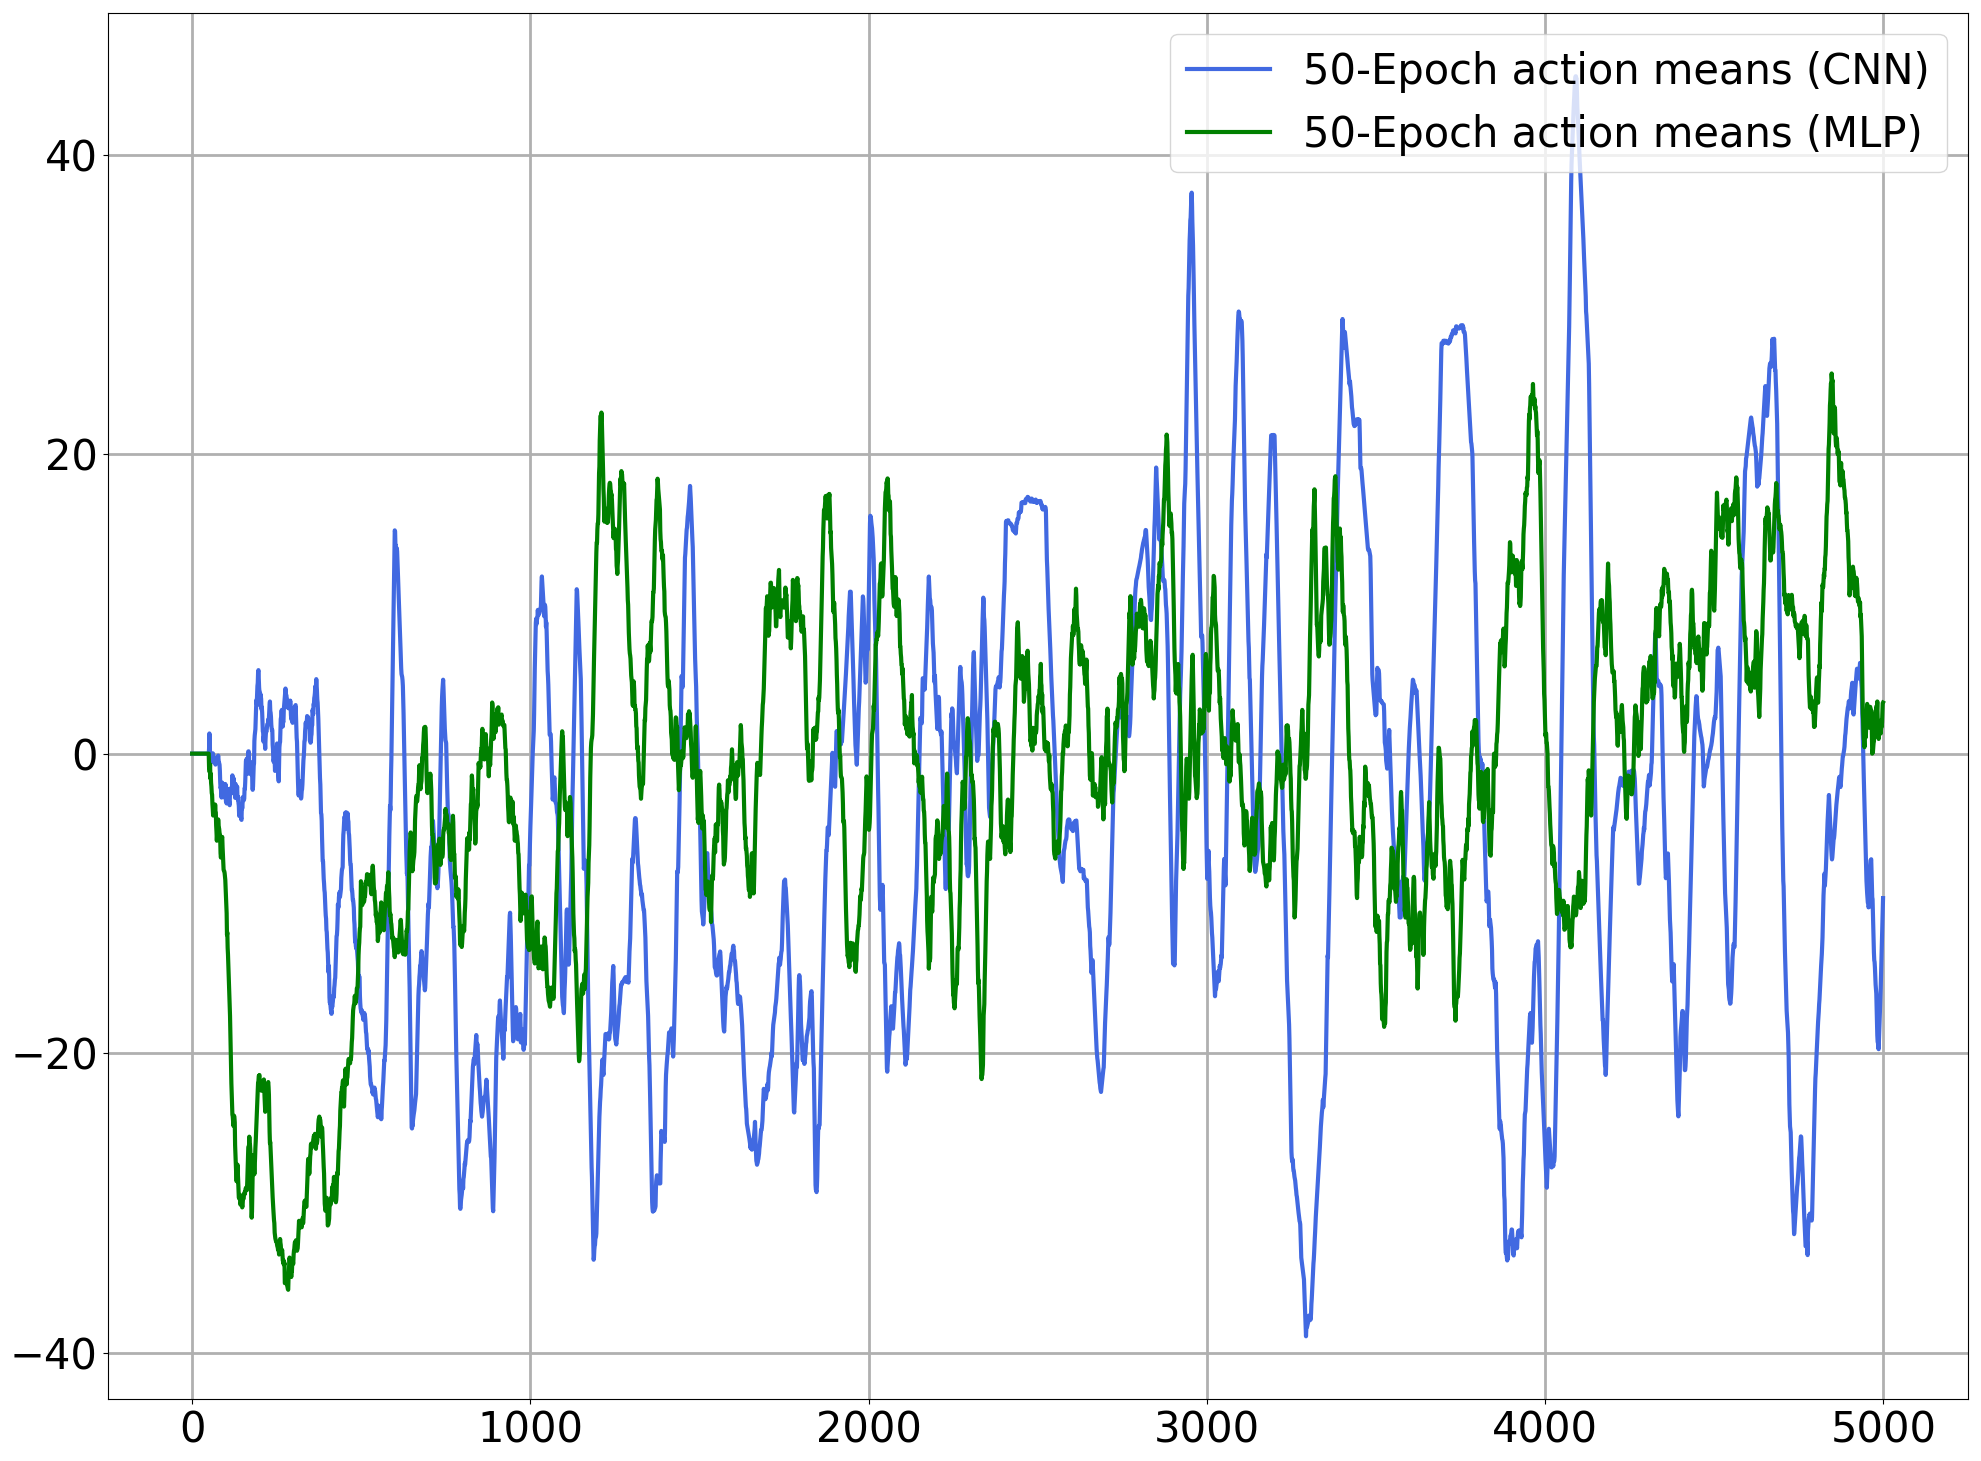
\includegraphics[width=\textwidth]{cnn_nn_1_sell_trades_mean_actions.png}
        \caption{Mean of actions per epoch (sell)}
        \label{fig:analysis-dqn-1-trades-action-sell}
    \end{subfigure}
    \caption{DQN agent rewards and mean of actions for buying and selling on training data set I using feature II.}
    \label{fig:analysis-dqn-1-trades}
\end{figure}

\begin{figure}[H]
    \centering
    \begin{subfigure}[b]{0.4\textwidth}
        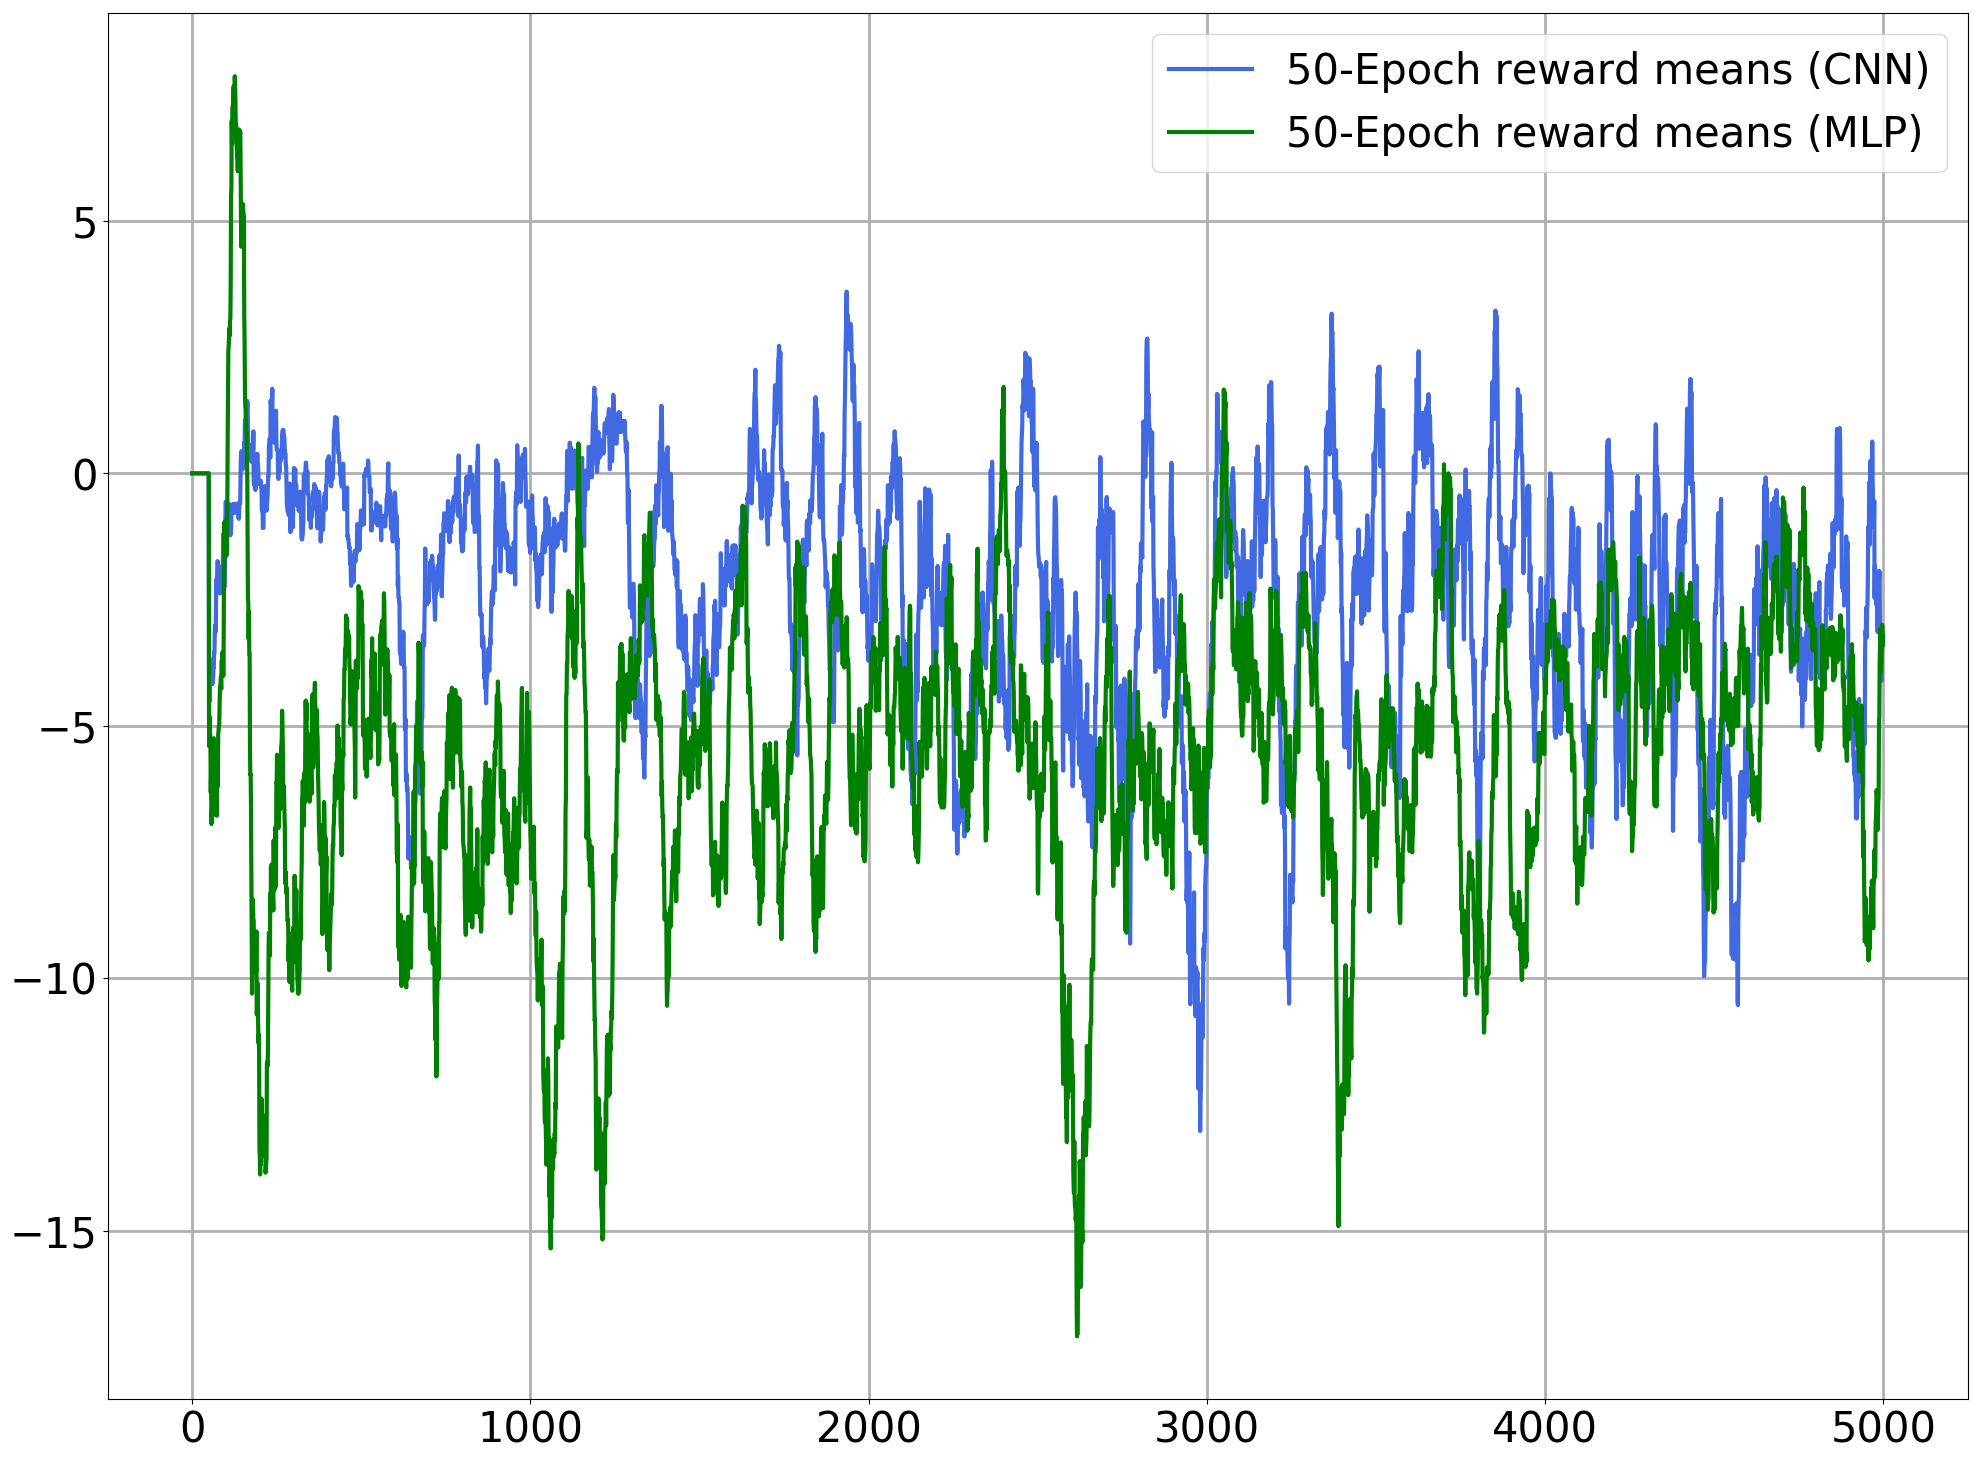
\includegraphics[width=\textwidth]{cnn_nn_2_buy_trades_rewards.png}
        \caption{Reward per epoch (buy)}
        \label{fig:analysis-dqn-2-trades-reward-buy}
    \end{subfigure}
    \begin{subfigure}[b]{0.4\textwidth}
        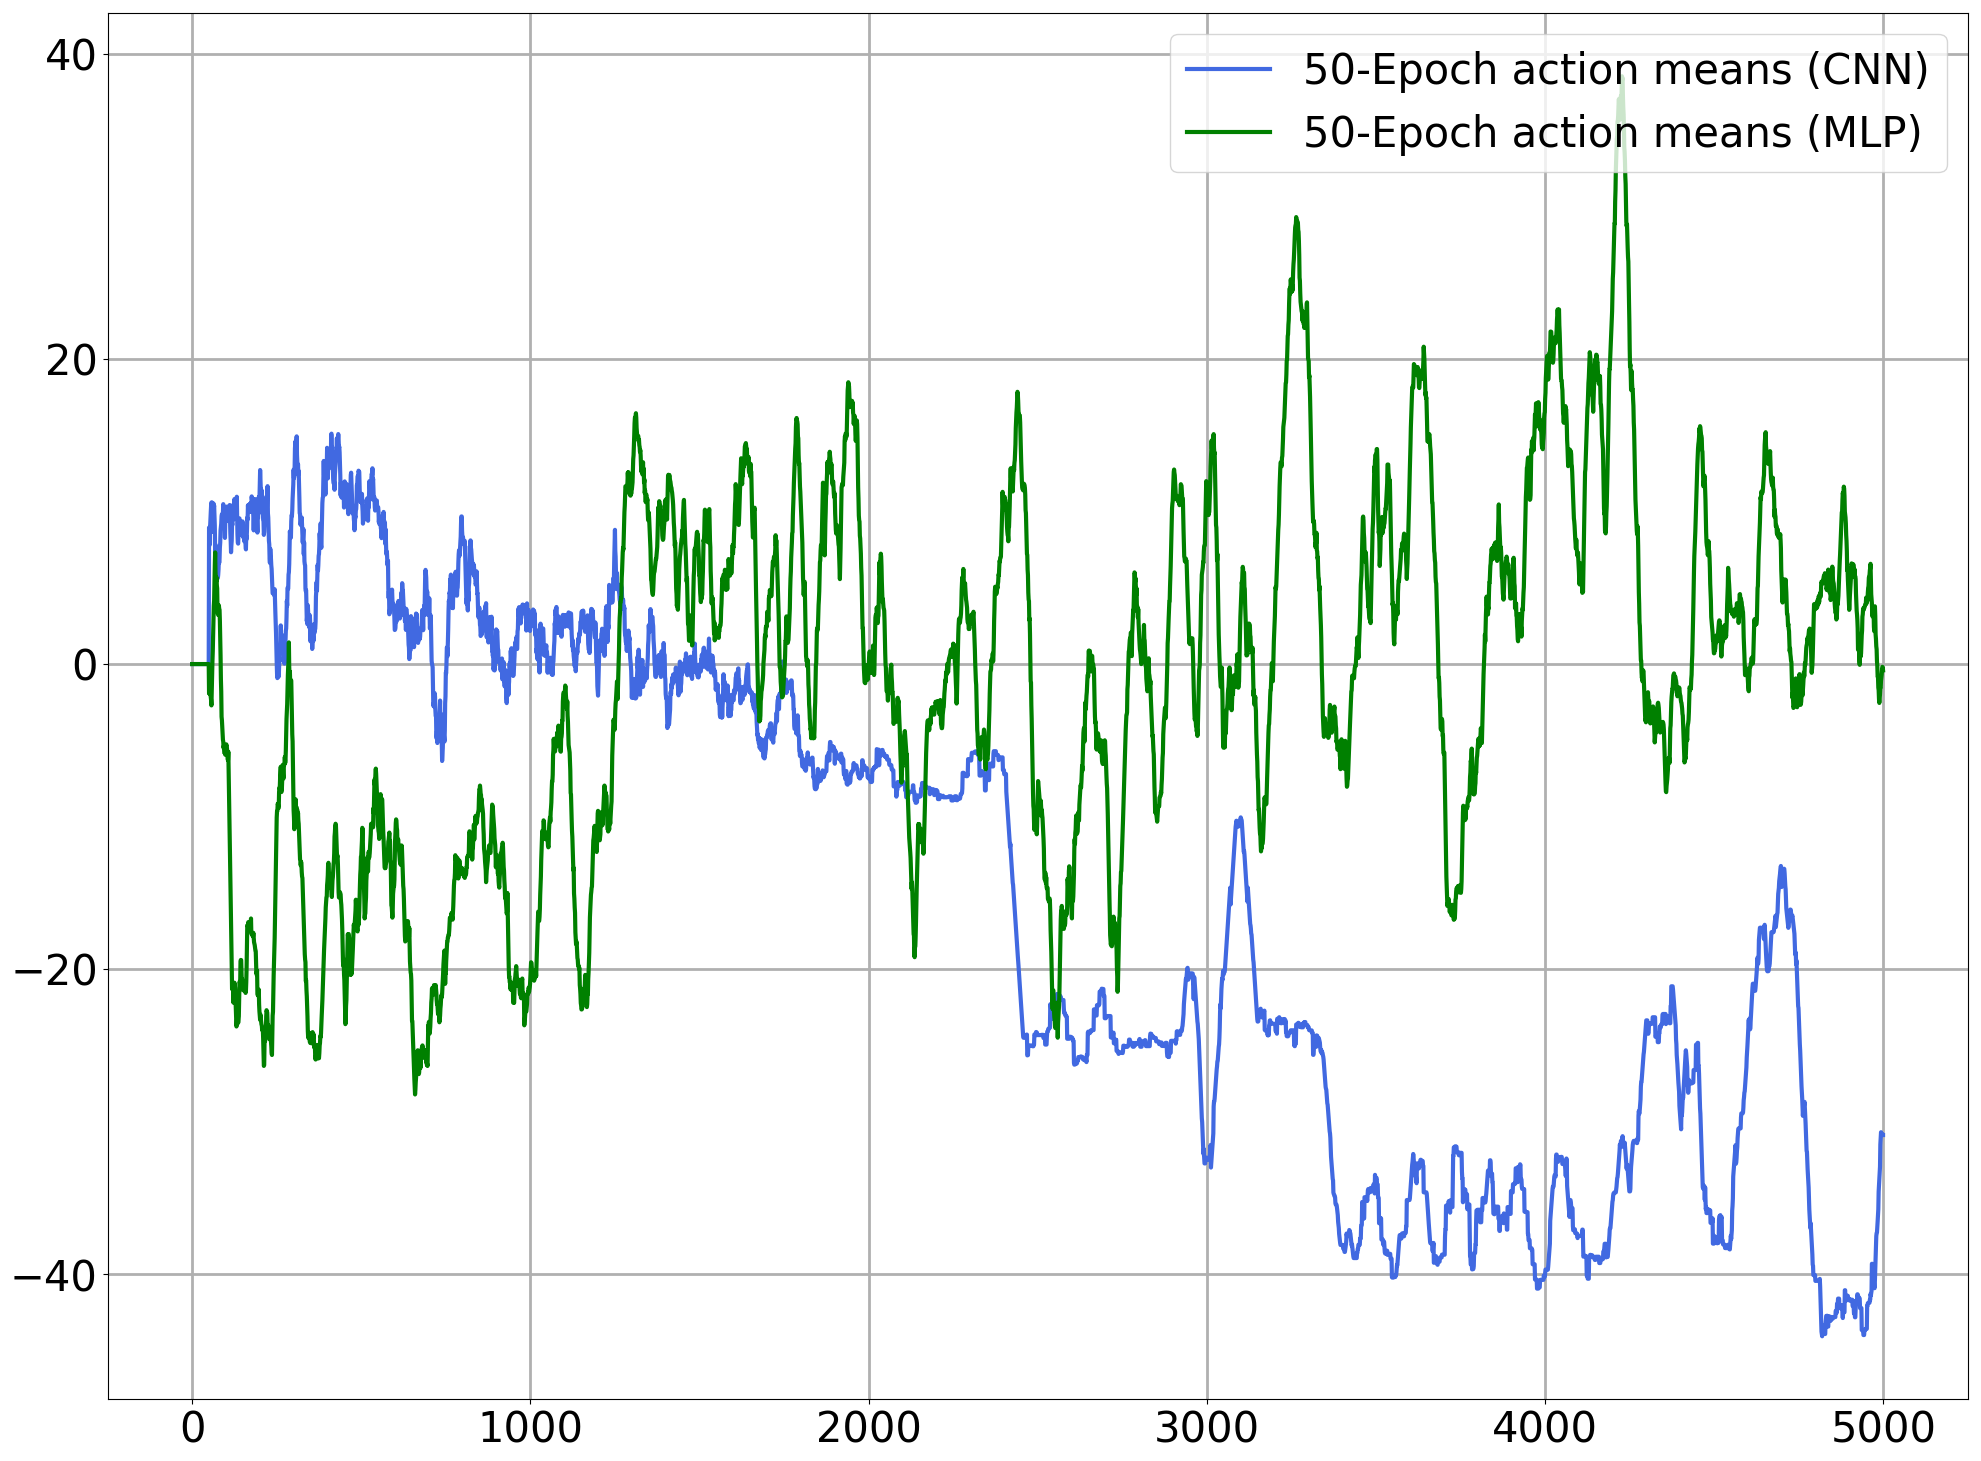
\includegraphics[width=\textwidth]{cnn_nn_2_buy_trades_mean_actions.png}
        \caption{Mean of actions per epoch (buy)}
        \label{fig:analysis-dqn-2-trades-action-buy}
    \end{subfigure}
    \begin{subfigure}[b]{0.4\textwidth}
        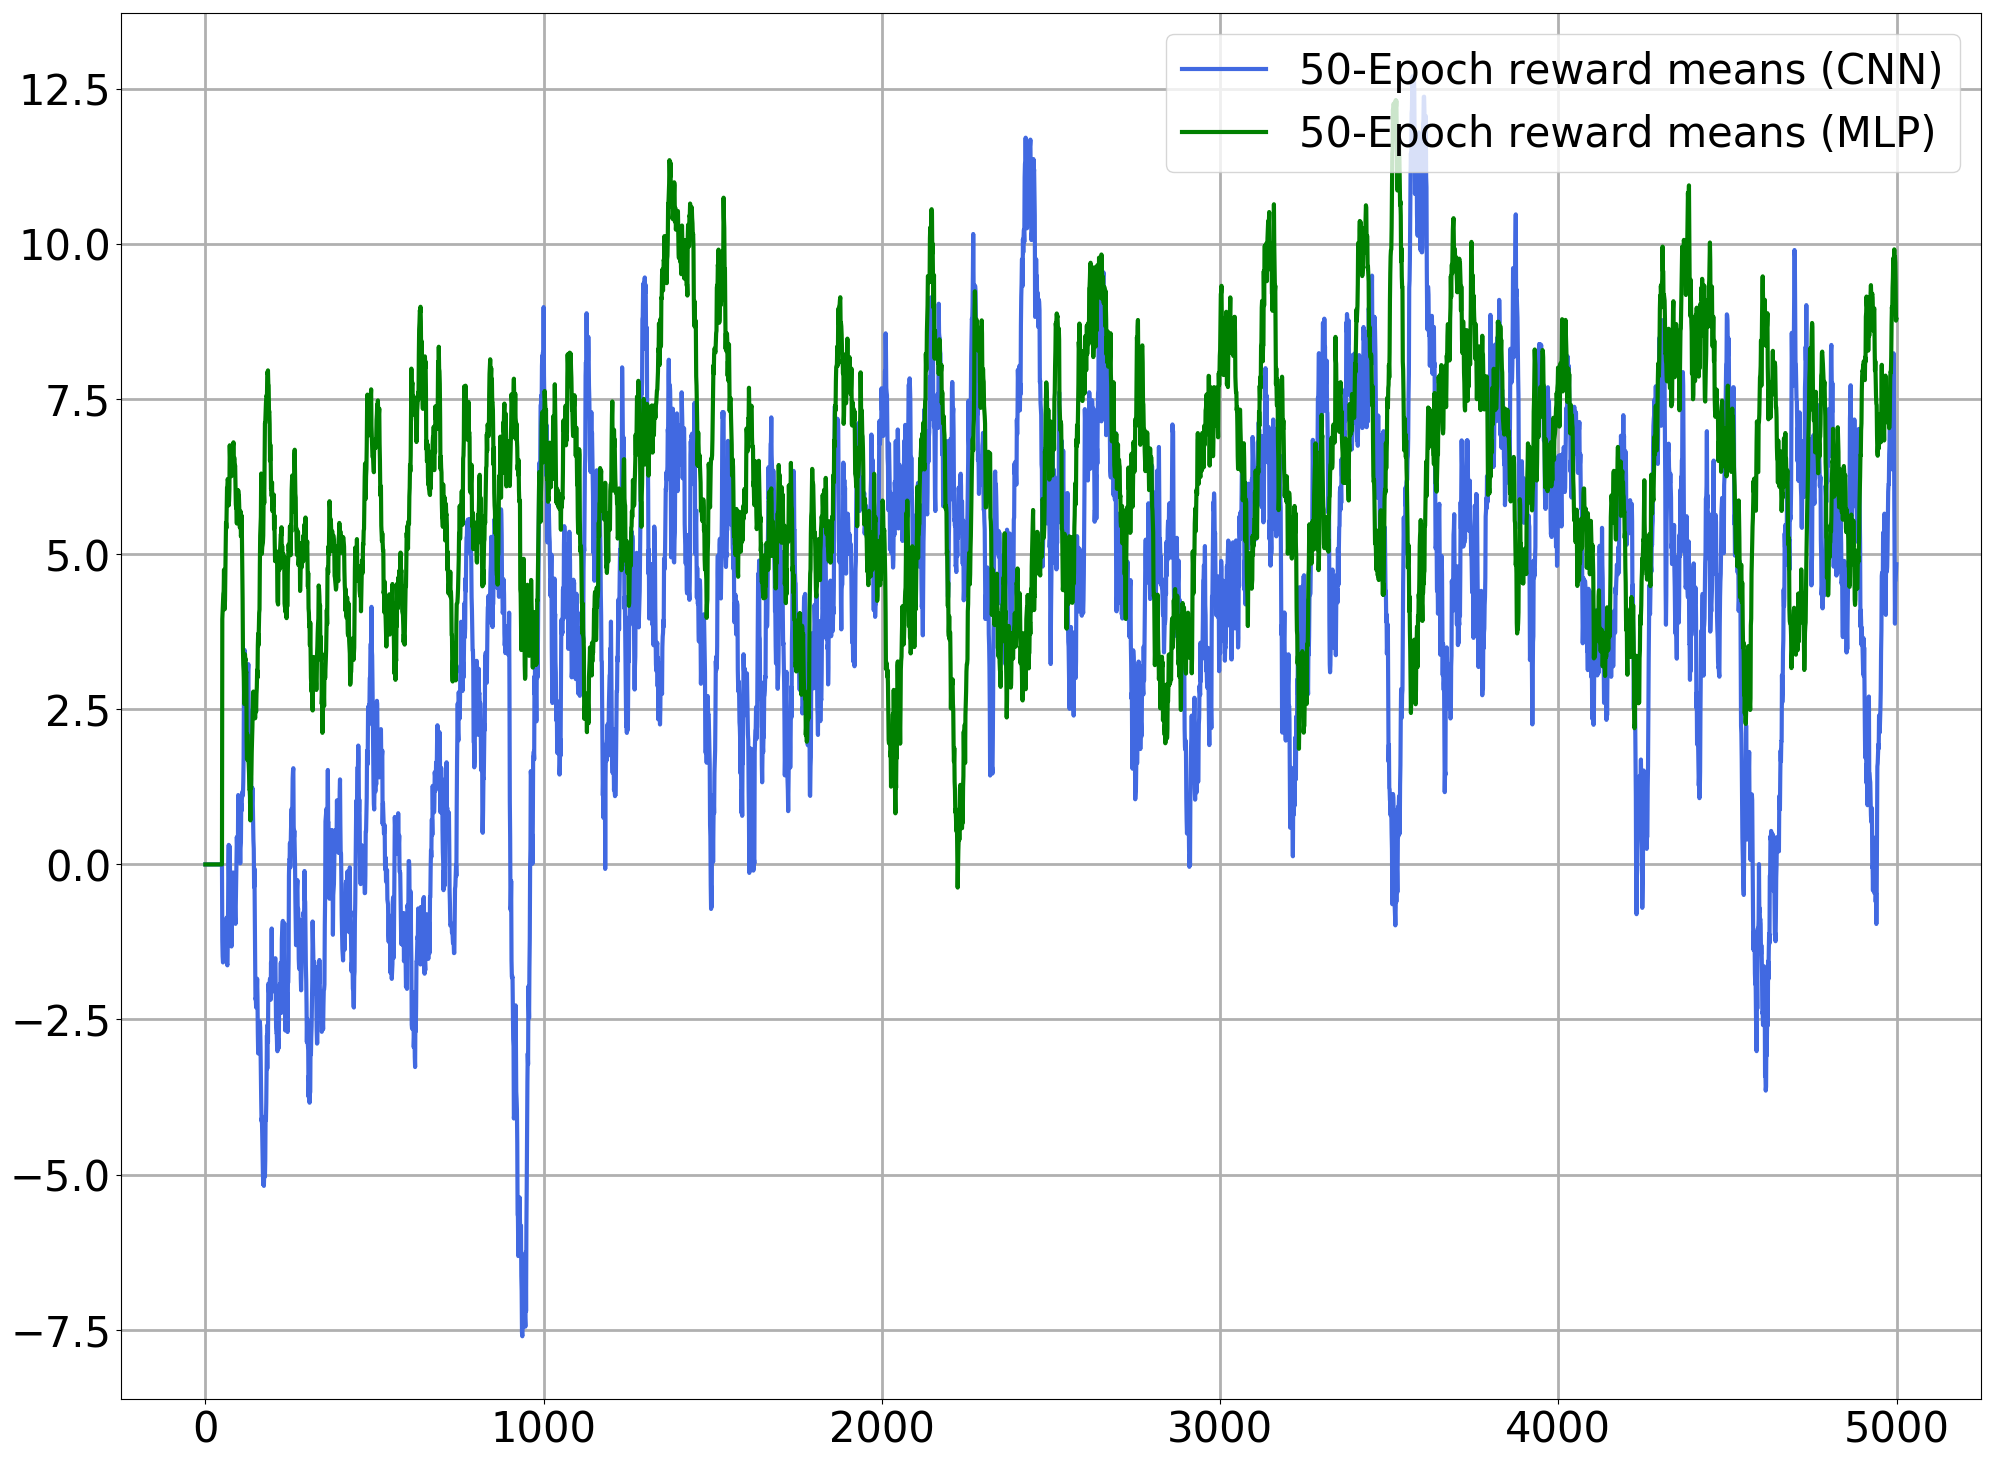
\includegraphics[width=\textwidth]{cnn_nn_2_sell_trades_rewards.png}
        \caption{Mean rewards per epoch (sell)}
        \label{fig:analysis-dqn-2-trades-reward-sell}
    \end{subfigure}
    \begin{subfigure}[b]{0.4\textwidth}
        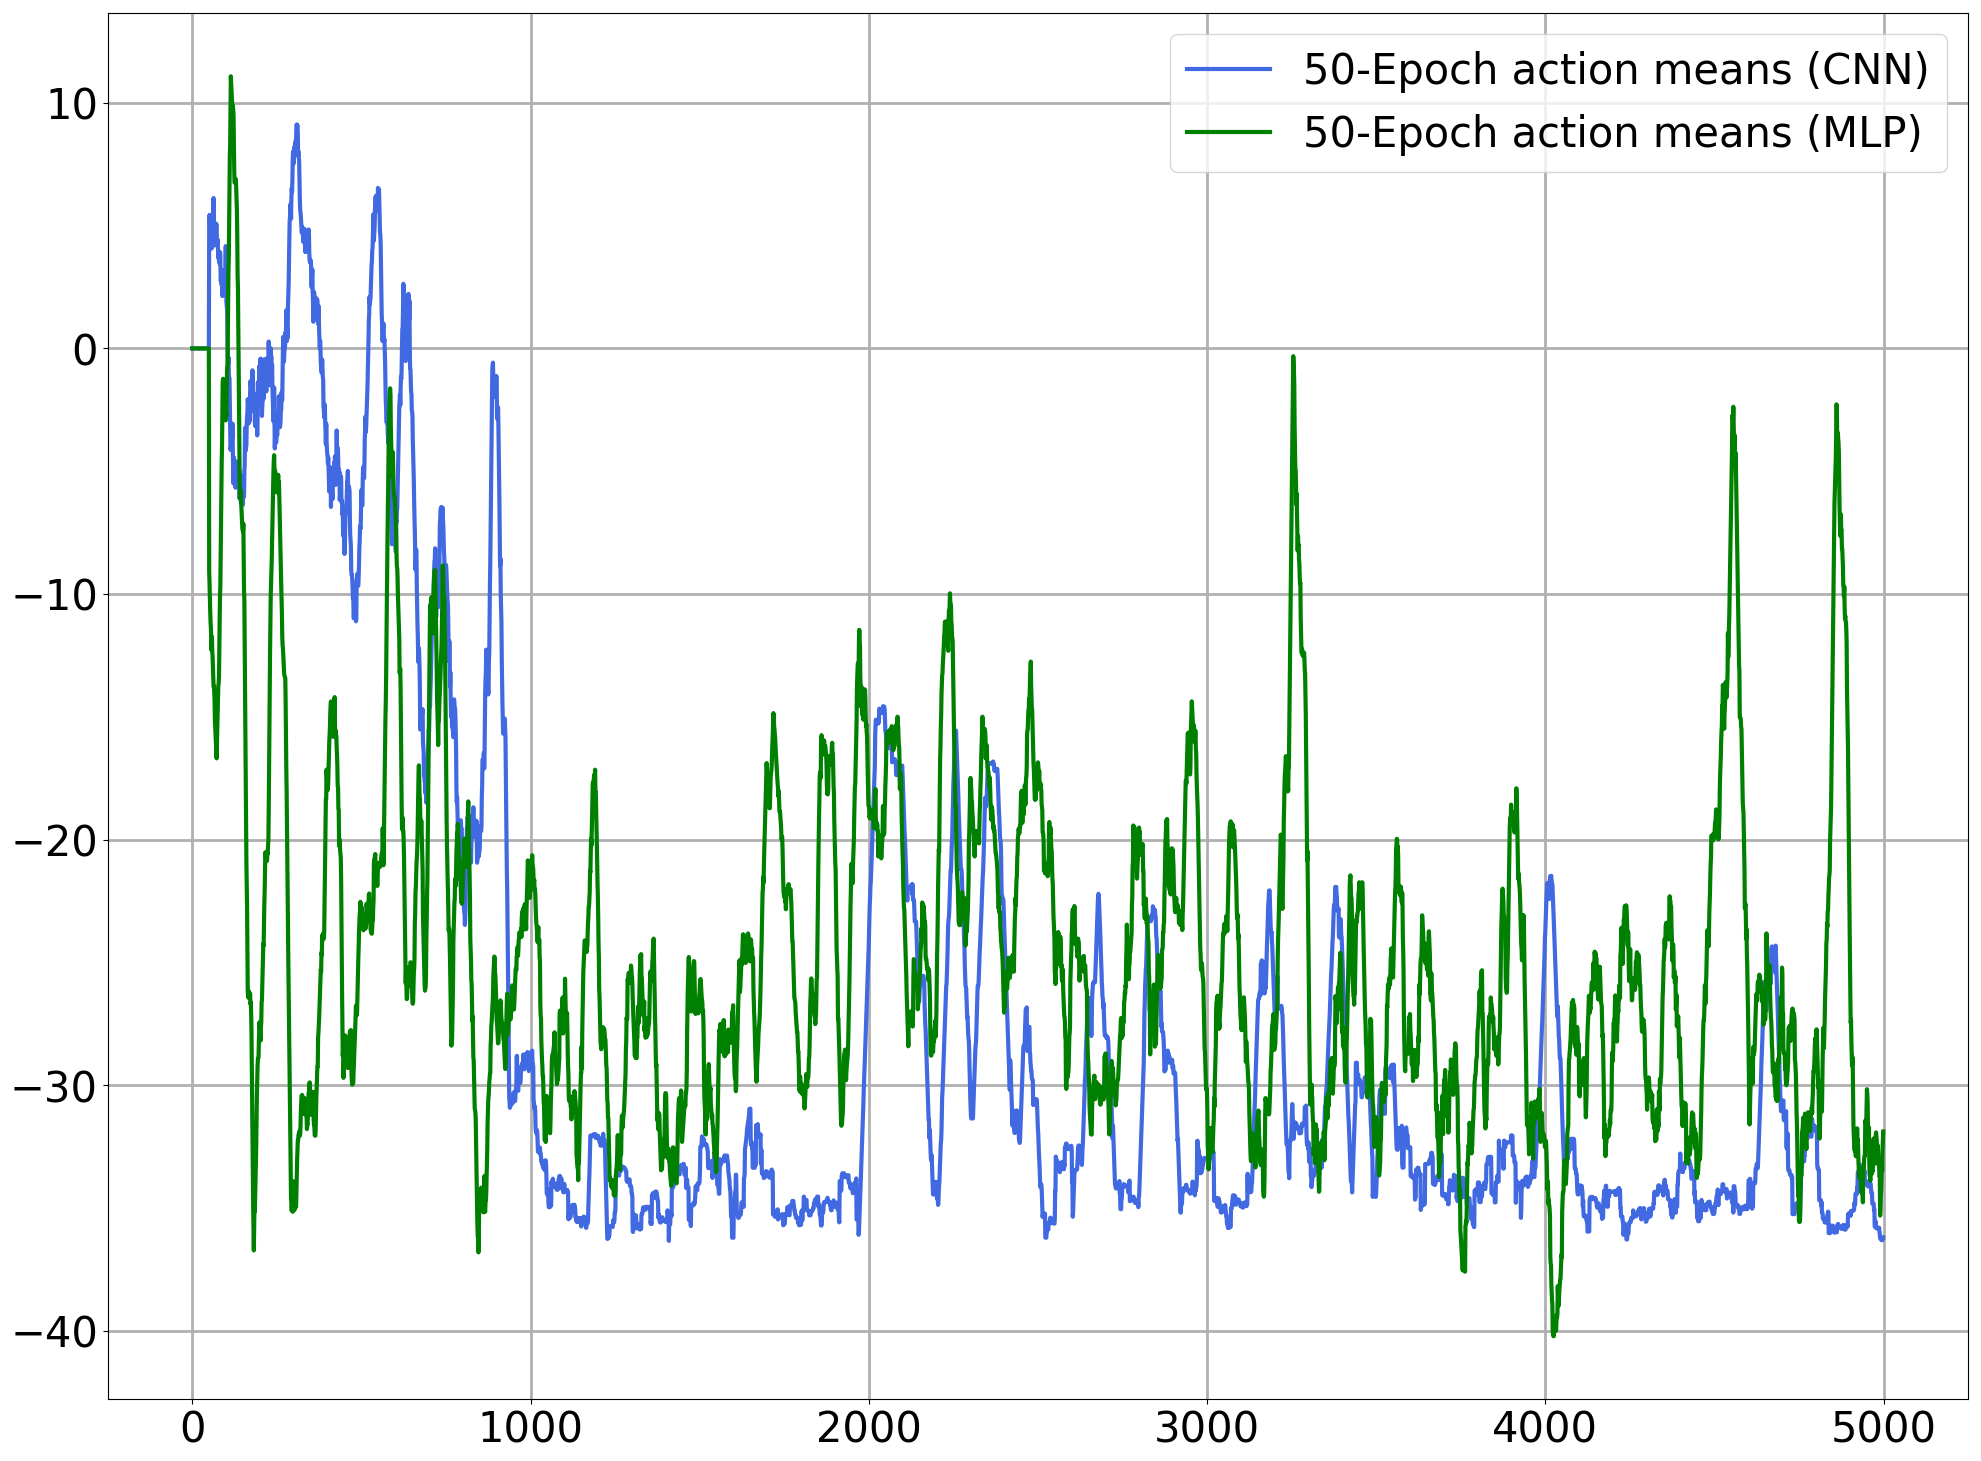
\includegraphics[width=\textwidth]{cnn_nn_2_sell_trades_mean_actions.png}
        \caption{Mean of actions per epoch (sell)}
        \label{fig:analysis-dqn-2-trades-action-sell}
    \end{subfigure}
    \caption{DQN agent rewards and mean of actions for buying and selling on training data set II using feature II.}
    \label{fig:analysis-dqn-2-trades}
\end{figure}

Figure \ref{fig:analysis-dqn-1-trades} illustrates the learning processes of the DQN agents when buying and selling in data set I.
As with the agents that were provided by Feature I, the rewards received when buying were slightly improved over the course of the 5000 epochs, which is shown in Figure \ref{fig:analysis-dqn-1-trades-reward-buy}.
Interestingly, the average action chosen per epoch by the DQN-CNN agent was abruptly adjusted after 4000 epochs, while the DQN-MLP's choice remained between 0 and 20, on average.
However, correlating improvements with respect to the rewards were not evident.
The rewards received when selling remained just below -10 for the DQN-CNN agent and below -20 for the DQN-MLP agent, as shown in Figure \ref{fig:analysis-dqn-1-trades-reward-sell}.
The average of the actions chosen by the DQN-CNN agent, though volatile, were adjusted towards becoming positive, as shown in Figure \ref{fig:analysis-dqn-1-trades-action-sell}.
Unfortunately, this is evidence that the average action does not provide enough insights into the actual decision-making process of the agent.
Had the agent consistently chosen positive actions throughout an epoch, an improvement in the reward would have been visible in the aforementioned figure.
Instead, the agent must have chosen negative actions in the initial steps and shifted towards very positive actions later in the epoch.
Figure \ref{fig:analysis-dqn-2-trades} illustrates the same learning process with the application of data set II.
The rewards for the buying process were not improved (Figure \ref{fig:analysis-dqn-2-trades-reward-buy}) for either of the two agents.
Interestingly, in this scenario, the DQN-MLP made a significantly better adjustment regarding the actions chosen (Figure \ref{fig:analysis-dqn-2-trades-action-buy}), indicating its willingness to make more immediate purchases.
Rewards for selling in data set II increased during the training, as shown in Figure \ref{fig:analysis-dqn-2-trades-reward-sell} and the average action chosen remained at around -30 after 1000 epochs, for both agents, as shown in Figure \ref{fig:analysis-dqn-2-trades-action-sell}.
\\
\\
Table \ref{tbl:analysis-dqn-tradefeature-summary} summarizes the average rewards received by the DQN agents during the backtest.
As with the previous application of Feature I to the DQN agents, significant optimization could be achieved when market conditions became more favorable to buying or selling.
For buying during falling market conditions (data set I), the DQN-CNN achieved a reward of 31.92 and the DQN-MLP a reward of 25.44, clear improvements compared to the expected market order return of -0.05.
Likewise, both agents improved sales in data set II (0.15 and 3.80 reward respectively).
Compared to when Feature I was applied, the agents under the application of Feature II achieved better results in difficult market conditions (selling in data set I and buying in data set II).
Particularly, sales in data set II were better than the expected returns of market orders.
Overall, as indicated by the positive sum of rewards achieved, both DQN agents were able to make purchases and sales of better than the market price.
Consequently, the rewards obtained were much better than the expected market order return.
The application of Feature II meant that the agent outperformed the DQN agent with Feature I (see Table \ref{tbl:analysis-dqn-orderfeature-summary} for comparison).
Thereby, it is evident that the DQN-CNN setup has yielded greater improvements than the DQN-MLP setup.

\begin{table}[H]
\centering
\begin{tabular}{l|l|l|l|}
\cline{2-4}
& \textbf{DQN-CNN} & \textbf{DQN-MLP} & \textbf{\begin{tabular}[c]{@{}l@{}}$\mathbb{E}$[Market\\ Order]\end{tabular}} \\ \hline
\multicolumn{1}{|l|}{\textbf{Buy (I)}}   & 31.92    & 25.44          & -0.05                                                           \\ \hline
\multicolumn{1}{|l|}{\textbf{Sell (I)}}  & -25.15   & -20.65         & -27.70                                                          \\ \hline
\multicolumn{1}{|l|}{\textbf{Buy (II)}}  & -3.56    & -6.43          & -1.06                                                           \\ \hline
\multicolumn{1}{|l|}{\textbf{Sell (II)}} & 0.15     & 3.80          & -1.72                                                           \\ \hline
\multicolumn{1}{|l|}{\textbf{$\Sigma$}} & 3.36      & 2.16          & -30.53                                                           \\ \hline
\end{tabular}
\caption{Summary of rewards during backtest of DQN agent using Feature II (historical trades).}
\label{tbl:analysis-dqn-tradefeature-summary}
\end{table}

\subsection{Comparison with different feature sizes}
\label{subsec:eval-comparison-feature-size}

Both features constructed in this project allow for size-related adjustments that determine the information content provided to the agent.
Until now, we have made use of one particular setting for each feature, that is, we have used $m_I=30$ windows with length $n_I=40$ for feature I and a vector length of $n_{II}=30$ for feature II.
With the use of the DQN-CNN agent, which has resulted in slightly better performance than the DQN-MLP agent, we will investigate whether or not a different size of the feature vector improve these results further.
We will proceed with the same evaluation as described in the previous two sections, but with different feature vector settings.
For feature I, we will investigate window sizes $m=10,20,30,40,50$ with maximum vector length $n=40$.
Similarly, for feature II, we will investigate the length of the vector $n=10,20,30,40,50$ (no window present for this feature).

Table \ref{tbl:analysis-dqn-featuresize} below shows the results from the backtest and confirms that the setting we ran earlier in this section performed the best.
It is evident that a smaller window size for feature I and a smaller vector length for feature II ($m_I<30$ and $n_{II}<30$) both have a negative impact on the resulting performance, indicating that the agent retrieved insufficient information.
However, increasing the dimensionality of our feature space ($m_I>30$ and $n_{II}>30$) did not improve the agents' capabilities and therefore indicates difficulties arising from the curse of dimensionality\cite{keogh2011curse}.

\begin{table}[H]
\centering
\begin{tabular}{|c|l|l|}
\hline
\textbf{\#}  & \multicolumn{1}{c|}{\textbf{\begin{tabular}[c]{@{}c@{}}Feature I\\ $\Sigma{[B1,S1,B2,BS2]}$\end{tabular}}} & \multicolumn{1}{c|}{\textbf{\begin{tabular}[c]{@{}c@{}}Feature II\\ $\Sigma{[B1,S1,B2,BS2]}$\end{tabular}}} \\ \hline
\textbf{10} & -36.85                                                                                                & -12.36                                                                                                 \\ \hline
\textbf{20} & -34.62                                                                                                & -13.68                                                                                                 \\ \hline
\textbf{30} & {\ul -18.62}                                                                                          & {\ul 3.36}                                                                                             \\ \hline
\textbf{40} & -21.59                                                                                                & -11.97                                                                                                 \\ \hline
\textbf{50} & -23.37                                                                                                & -1.43                                                                                                  \\ \hline
\end{tabular}
\caption{Summary of rewards during backtest of DQN-CNN agent using different feature sizes.}
\label{tbl:analysis-dqn-featuresize}
\end{table}

\section{Determining the limitations of the DQN agent}
\label{sec:eval-dqn-limitations}
This section aims to determine the capabilities and limitations of the DQN agent with the use of Feature I in greater detail.
Sample order submissions are investigated which uncover the actions chosen by an agent throughout one epoch.
Therefore, we will be able to see which market situations prevented the agent from achieving a positive reward and conclude why the agent was not able to choose the most appropriate actions.
In addition, artificial order books are being created which serve as new data sets to train and test the DQN agent on.
With their aid, we aim to determine the capabilities of the deep reinforcement learning technique under market conditions which are 1) not affected by short-term fluctuations and 2) a hold constant spread between best bid and best ask is given.

\subsection{Limitation arising from market situations or inappropriate actions from the agent}
Extensive investigations have shown that the DQN agent fails to place orders that lead to constant positive rewards for the following two reasons: 1) when the market situation does not allow the agent to do so and 2) when the agent submits an inappropriate action.

Our investigations have shown that, for the first category, it is not just upwards and downwards trends which make it difficult for the order placement to result in a positive reward, but also when the spread between the best bid and best ask price becomes large.
Examples of wide spread scenarios are shown in Figures \ref{fig:analysis-limit-wide-spread-buy} and \ref{fig:analysis-limit-wide-spread-sell}, where an agent attempted the placement of a buy and sell order respectively.
\begin{figure}[H]
    \centering
    \makebox[\linewidth]{
        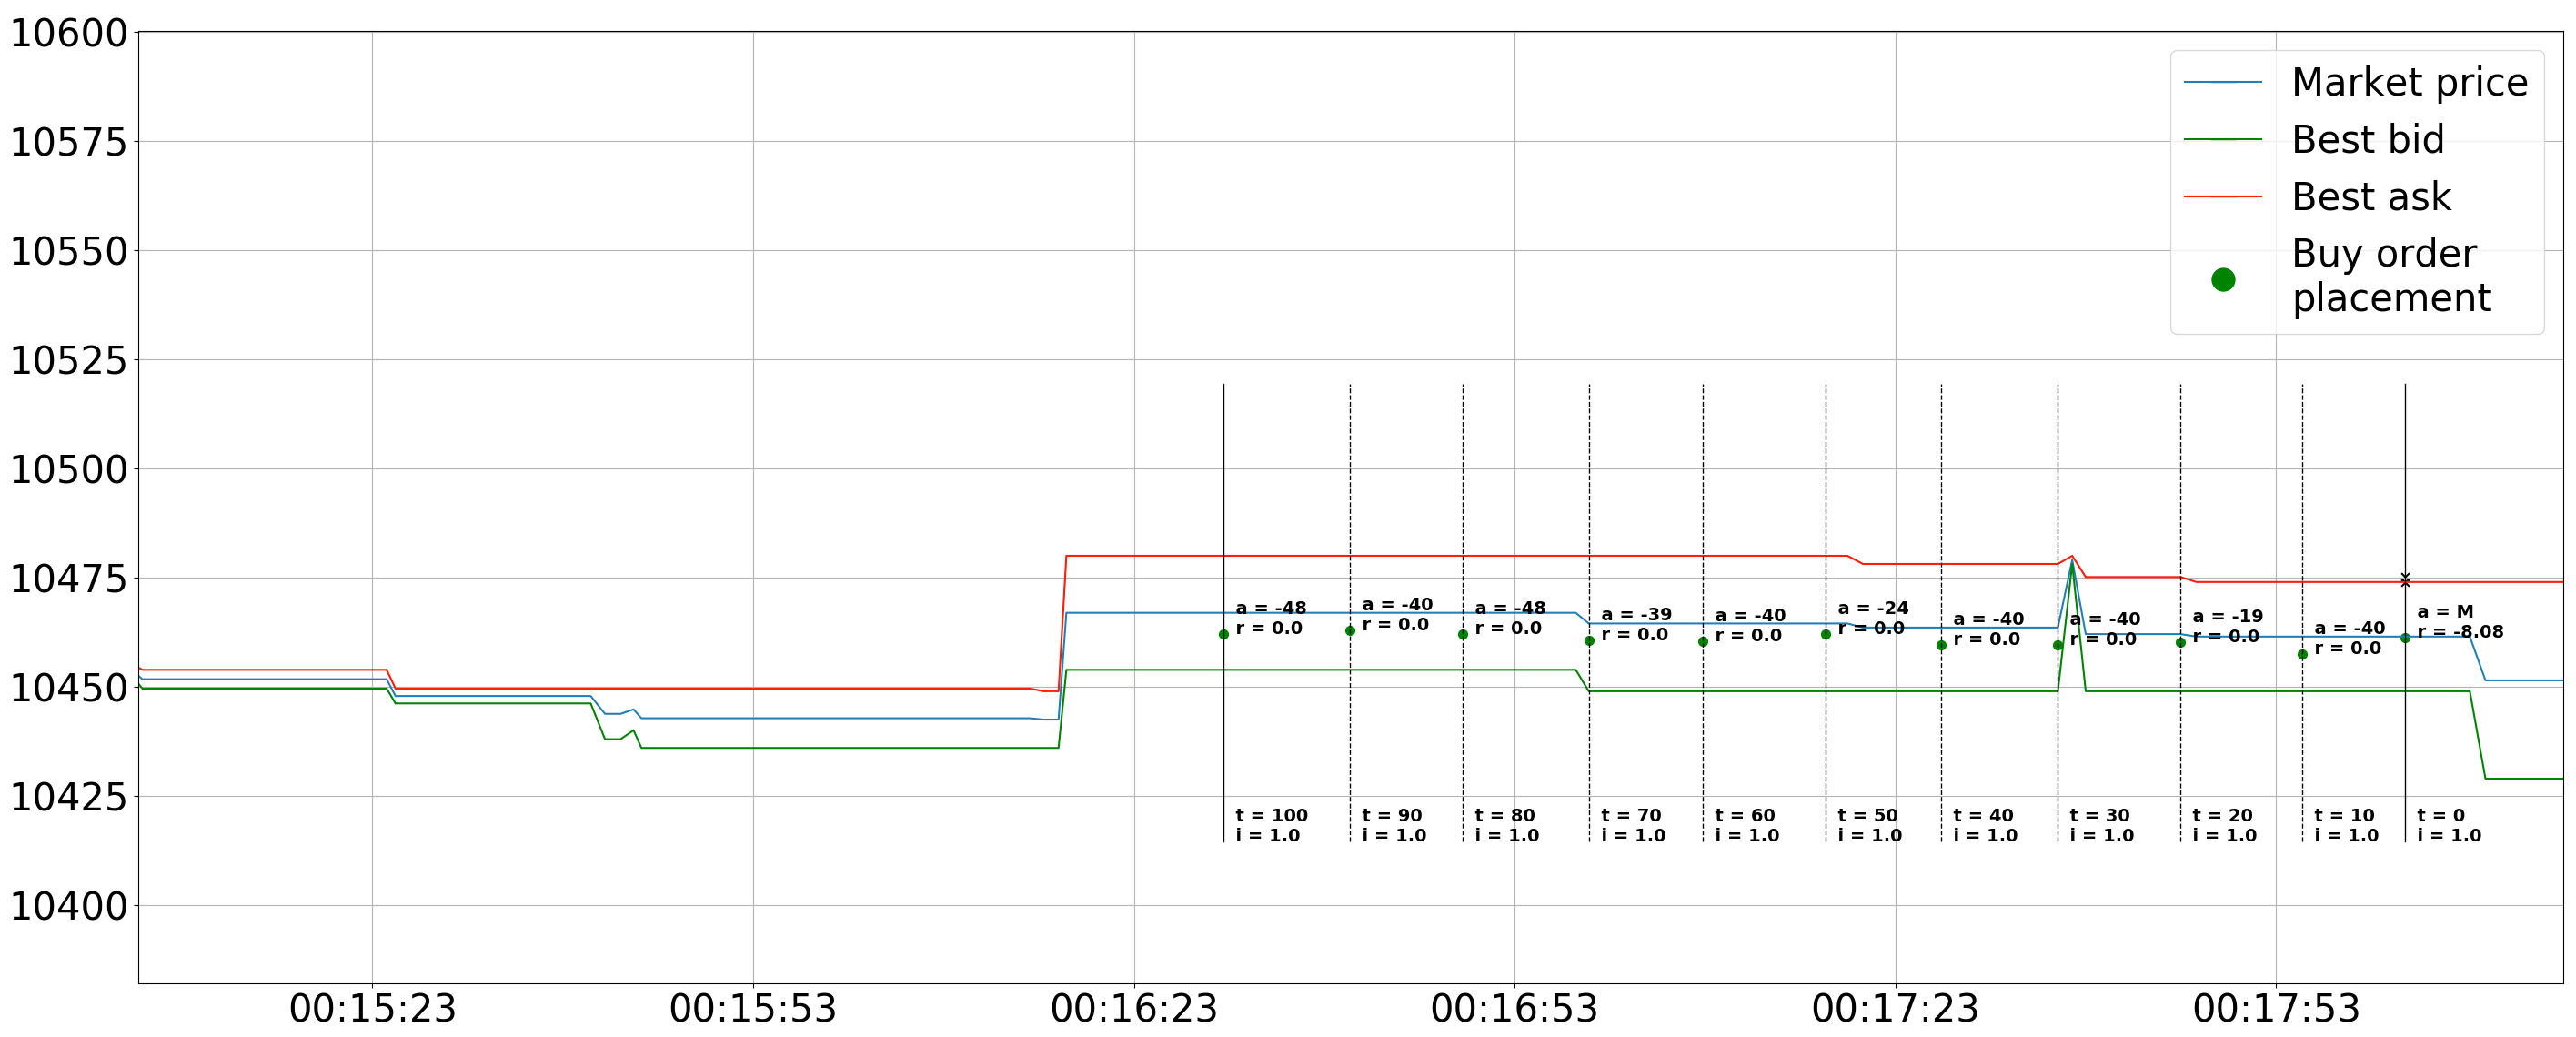
\includegraphics[width=\textwidth]{images/analysis-limit-wide-spread-buy}
    }
    \caption{Wide spread between bid and ask prevents agent from buying.}
    \label{fig:analysis-limit-wide-spread-buy}
\end{figure}
\begin{figure}[H]
    \centering
    \makebox[\linewidth]{
        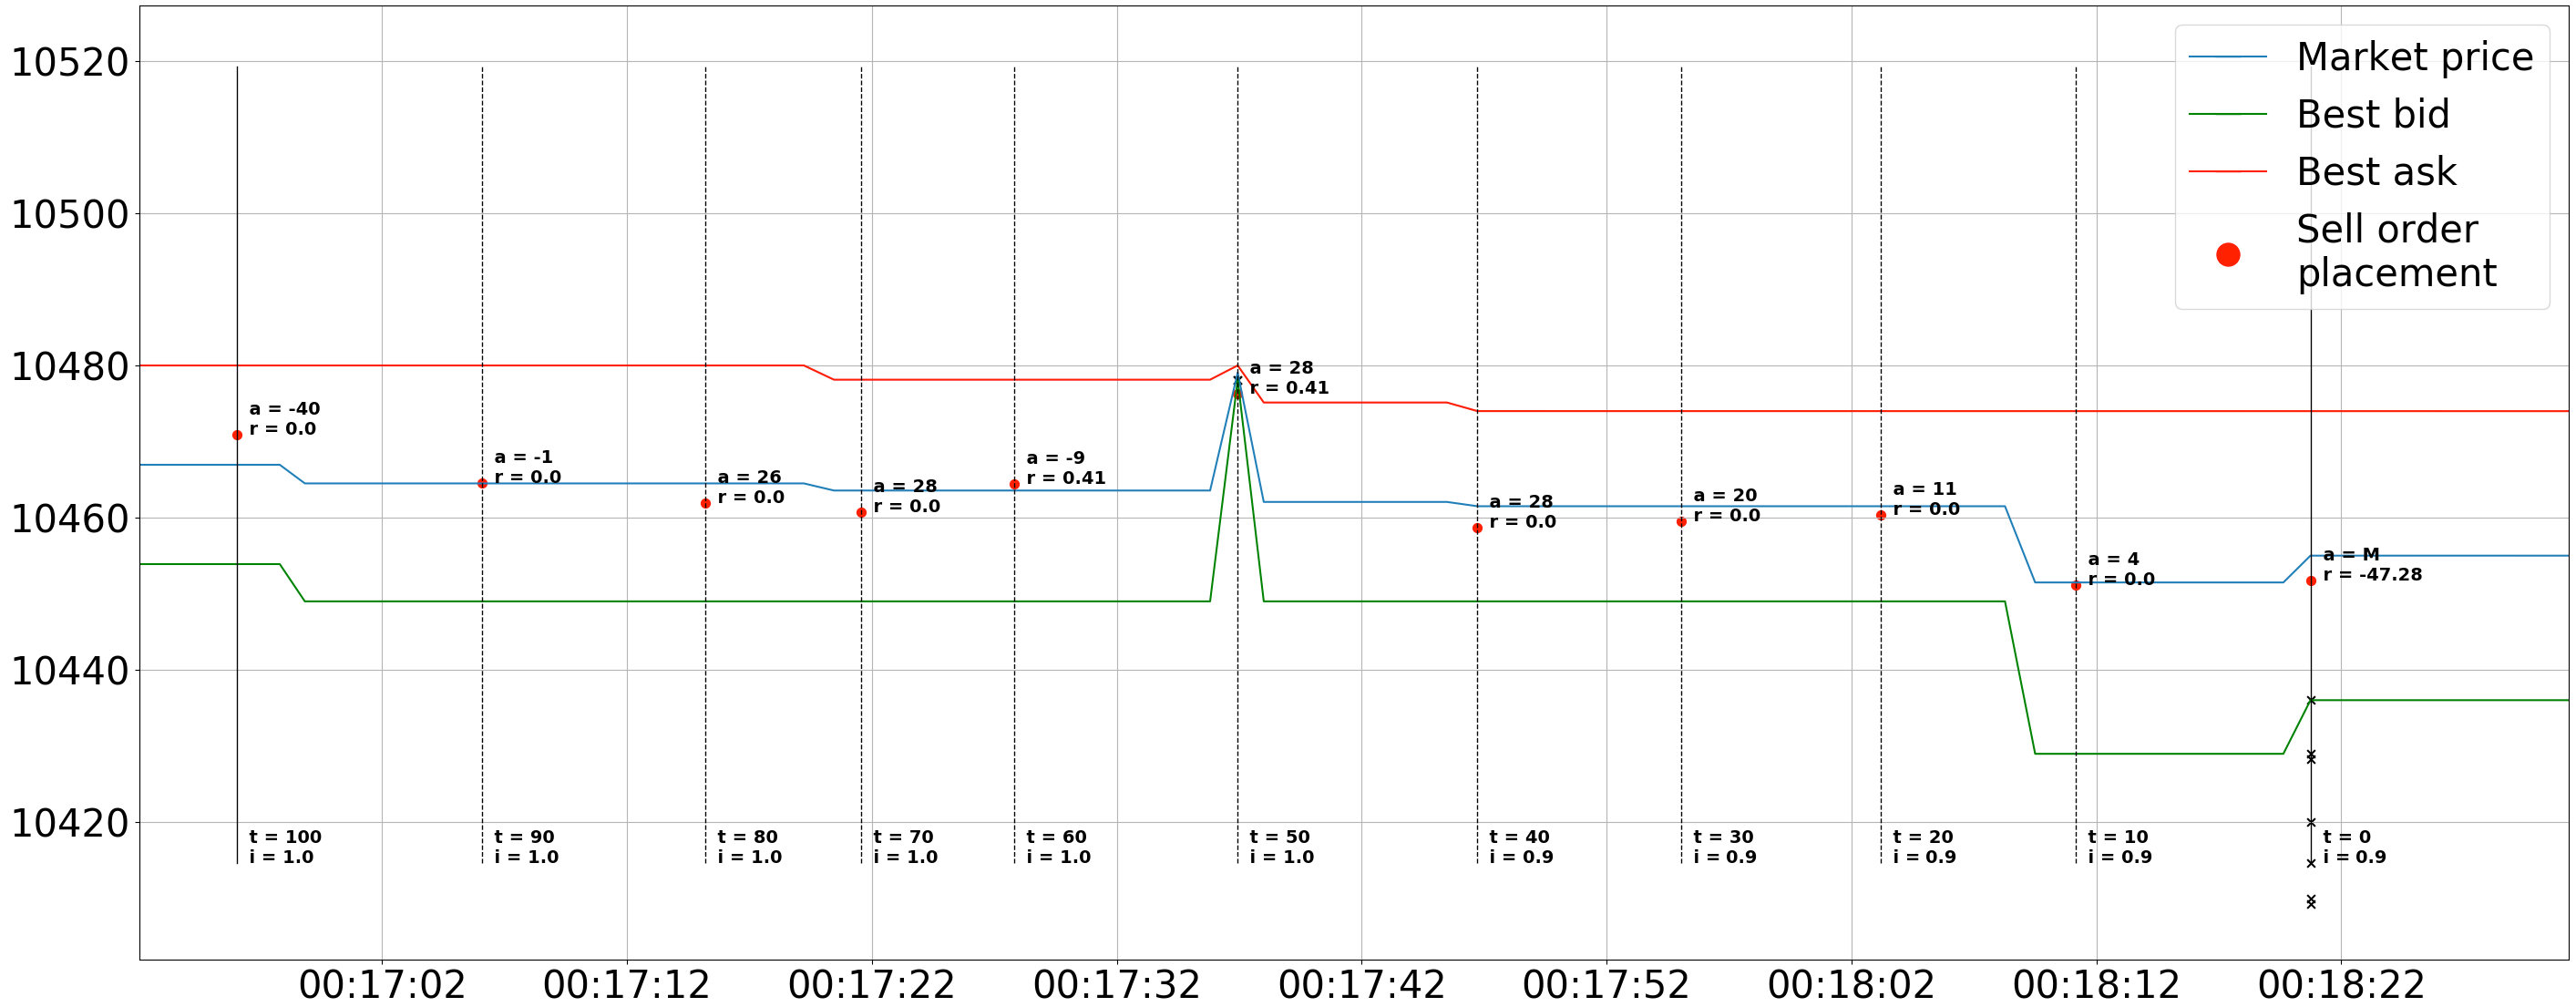
\includegraphics[width=\textwidth]{images/analysis-limit-wide-spread-sell}
    }
    \caption{Wide spread between bid and ask prevents agent from selling.}
    \label{fig:analysis-limit-wide-spread-sell}
\end{figure}
Prior to the start of the buy order placement, the spread between the best bid and best ask price was very close, as indicated by the green and red lines.
However, during the placement of this order, the spread widened and remained larger than \$50.00 for almost the entire time horizon.
Since the actions are segmented into discrete steps of $\Delta{a}=0.10$, with a total of 101 steps, and a market price ranging from -\$5.00 to +\$5.00, the agent had no chance of placing the orders close to the best ask price.
As a result, the entire inventory of 1.0 BTC bought by using a market order at the end of the time horizon (a trade is marked with a cross).
This generated a negative reward of -8.08.
The same market situation is demonstrated during which the agent initiated the process of placing a sell order.
Similarly, the price level was close to the best bid price only once.
As a result, a market order followed in which the agent sold the remaining 0.9 BTC at a decreased price that resulted in a negative reward of -47.28.
In addition, since there was not much liquidity offered by buyers, the market order was partially filled at decreasing price levels, as indicated by the crosses in the figure.
Two possible ways to overcome this limitation would be to either increase the number of steps or to increase the action step size; both approaches will be addressed in Chapter \ref{chap:discussion}.
\begin{figure}[H]
    \centering
    \makebox[\linewidth]{
        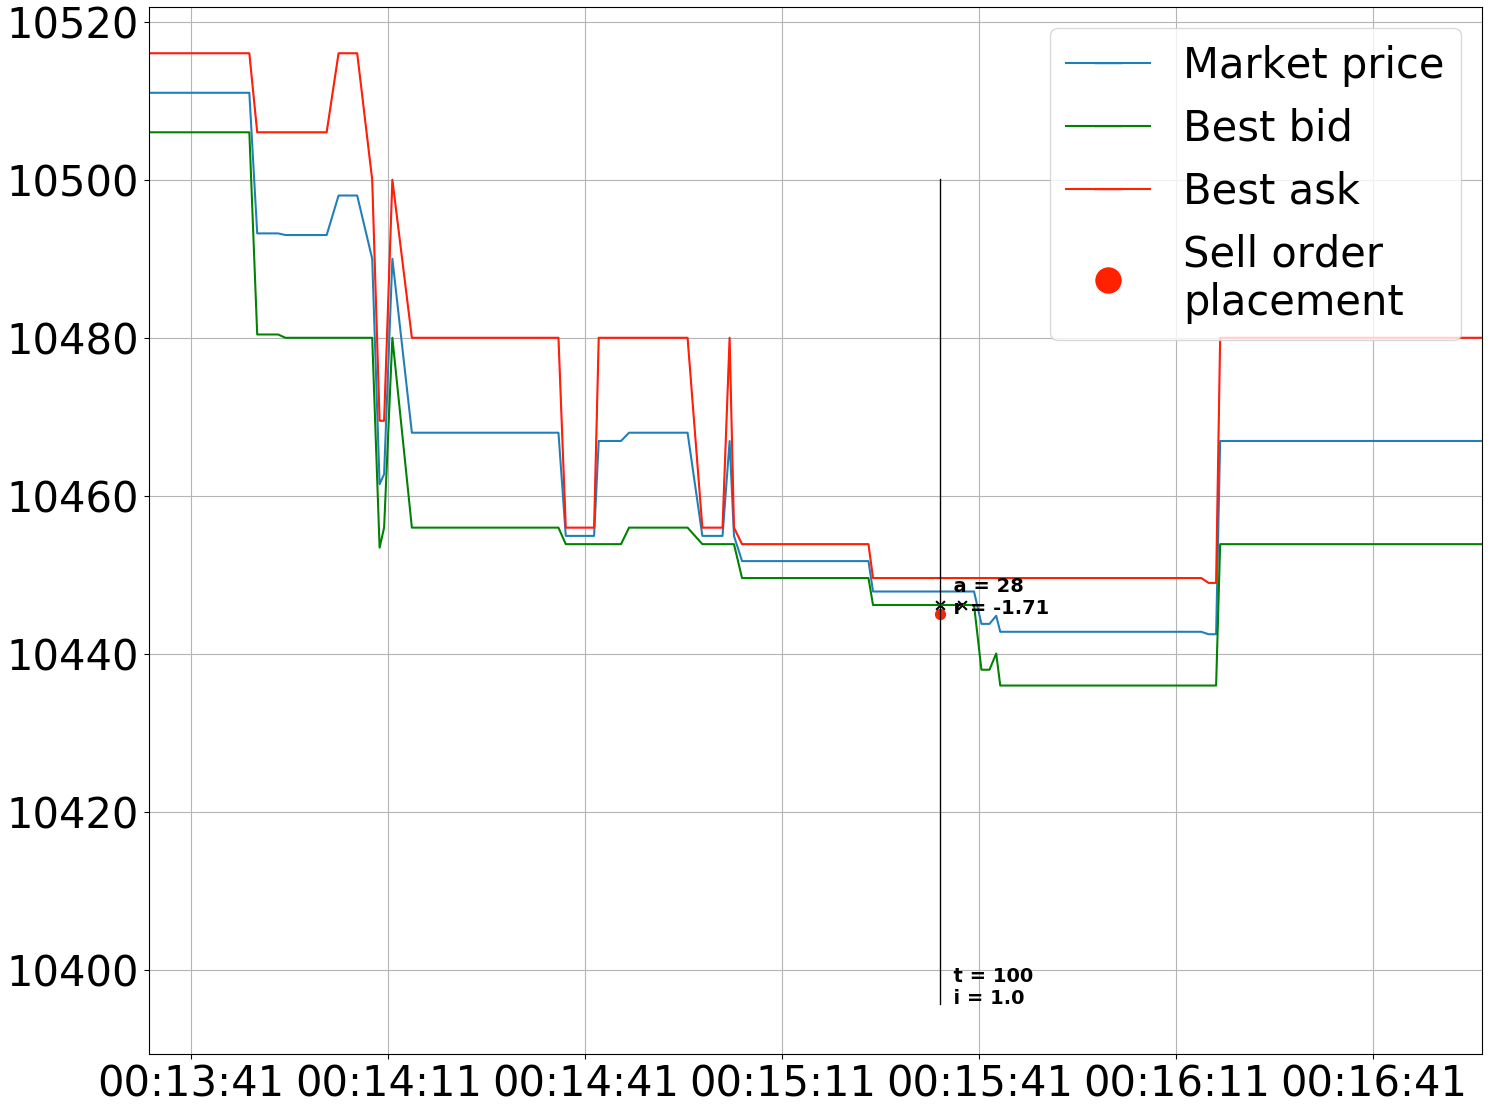
\includegraphics[width=10cm]{images/analysis-limit-impatient}
    }
    \caption{Wide spread between bid and ask prevents agent from selling.}
    \label{fig:analysis-limit-impatient}
\end{figure}
An example of the second category, where the agent clearly failed to select an appropriate action, is shown in Figure \ref{fig:analysis-limit-impatient}.
As is illustrated, the market price, and the best bid and ask price were declining before the initialization of the sell order placement. 
The agent then decided to cross the spread in the first step and choose action 28, which meant that it was willing to sell for \$2.80 below the market price.
By doing this, the order was immediately filled and resulted in a negative reward of -1.71.
Ideally, the agent should have been more patient and decided to place a limit order below the spread.
Then, in a subsequent step, the order could have been filled by means of a negative action, which would have resulted in a positive reward.
It is assumed that the agent failed to generalize the development of the order book with the provided feature set.
Instead, the agent reacted to the previous, declining market situation, in which  the better choice would certainly have been to immediately fill the sell order.

\subsection{Capabilities evaluated using artificial limit order books}

Introducing an artificially created order book allows us to determine the capabilities of a reinforcement learning agent in greater detail.
We define the formation of the order book states over time and therefore can calculate the optimal order placement policy in advance.
In doing this, we can investigate whether or not an agent is able to find the optimal placement policy.
In addition, by constructing artificial order books, we were able to remove any short-term market fluctuations and therefore provide more consistent rewards to the agent during training.
Figure \ref{fig:eval-limit-artificial} below shows the setup of two such order books.
Both consist of 10 minutes worth of data with order book states changing every 1 second, resulting in a total of 600 data points that represent the order book states.
Every such state consists of 25 levels on both the bid and ask side with a deviation of \$0.10 for each level, as shown in the zoomed panes.
In addition, on every such level, 1.0 BTC is listed on the bid and ask side, which ensures that an agent can fill the entire order at any chosen limit level.
The change in the order book states is then determined by a function.
\begin{figure}[H]
    \centering
    \begin{subfigure}[b]{0.45\textwidth}
        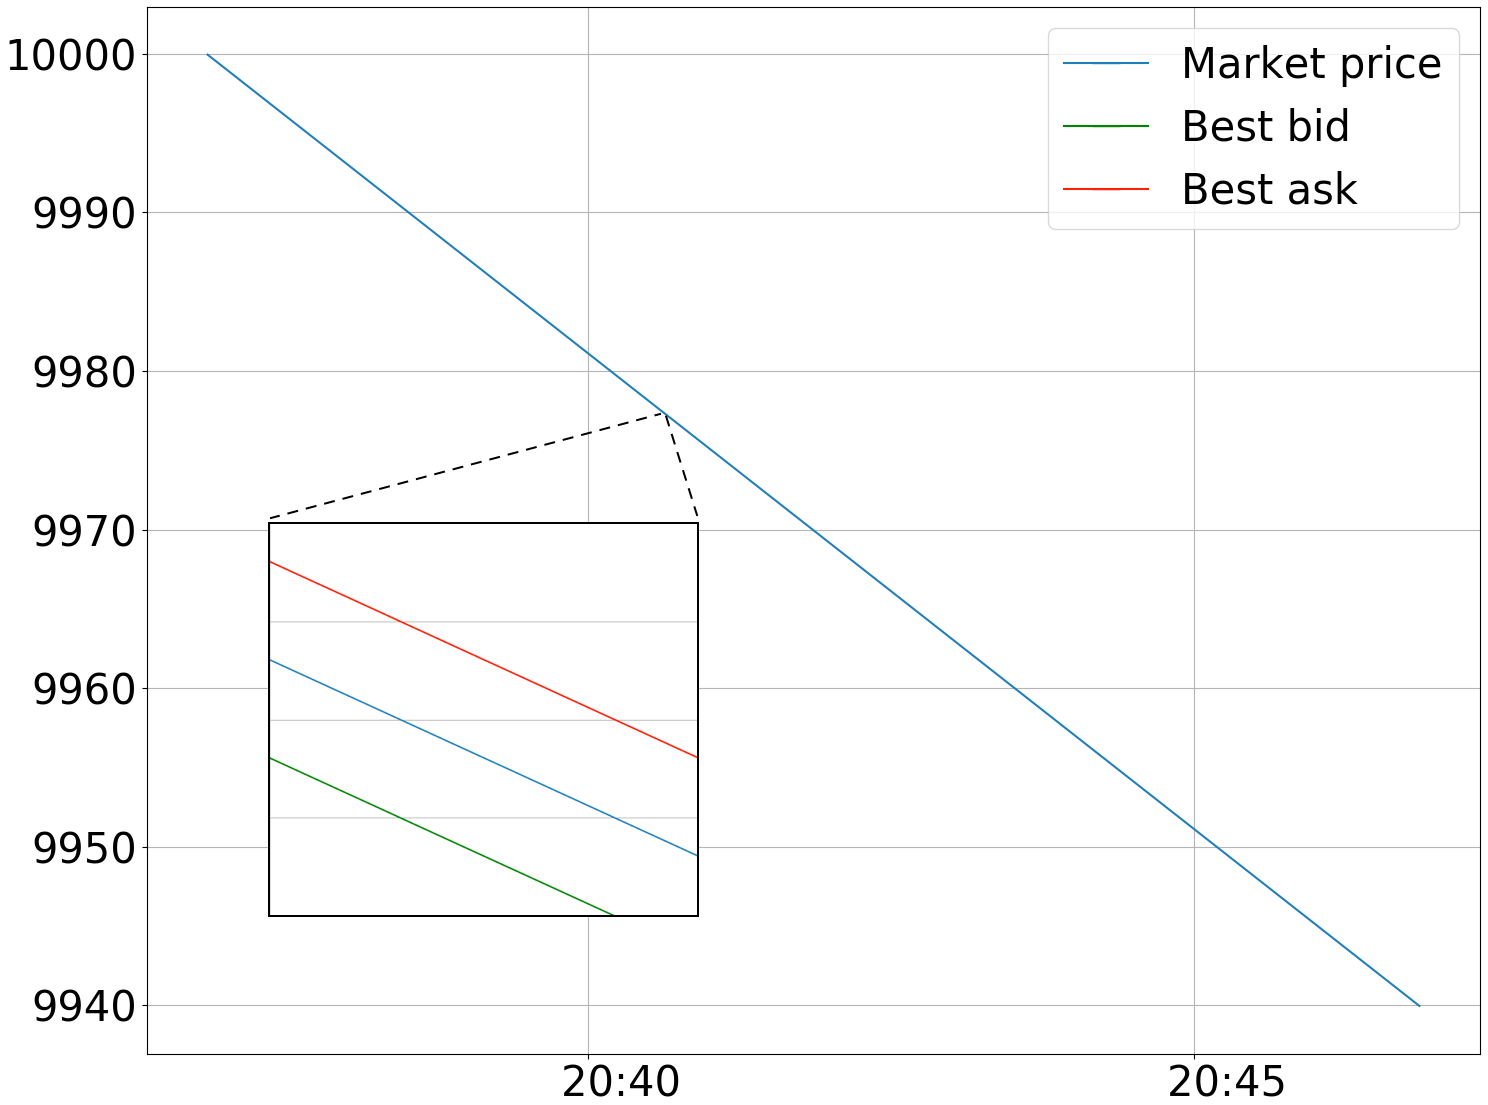
\includegraphics[width=\textwidth]{eval-limit-down}
        \caption{Linear configuration of order book states with slope $a=-0.1$}
        \label{fig:eval-limit-down}
    \end{subfigure}
    \begin{subfigure}[b]{0.45\textwidth}
        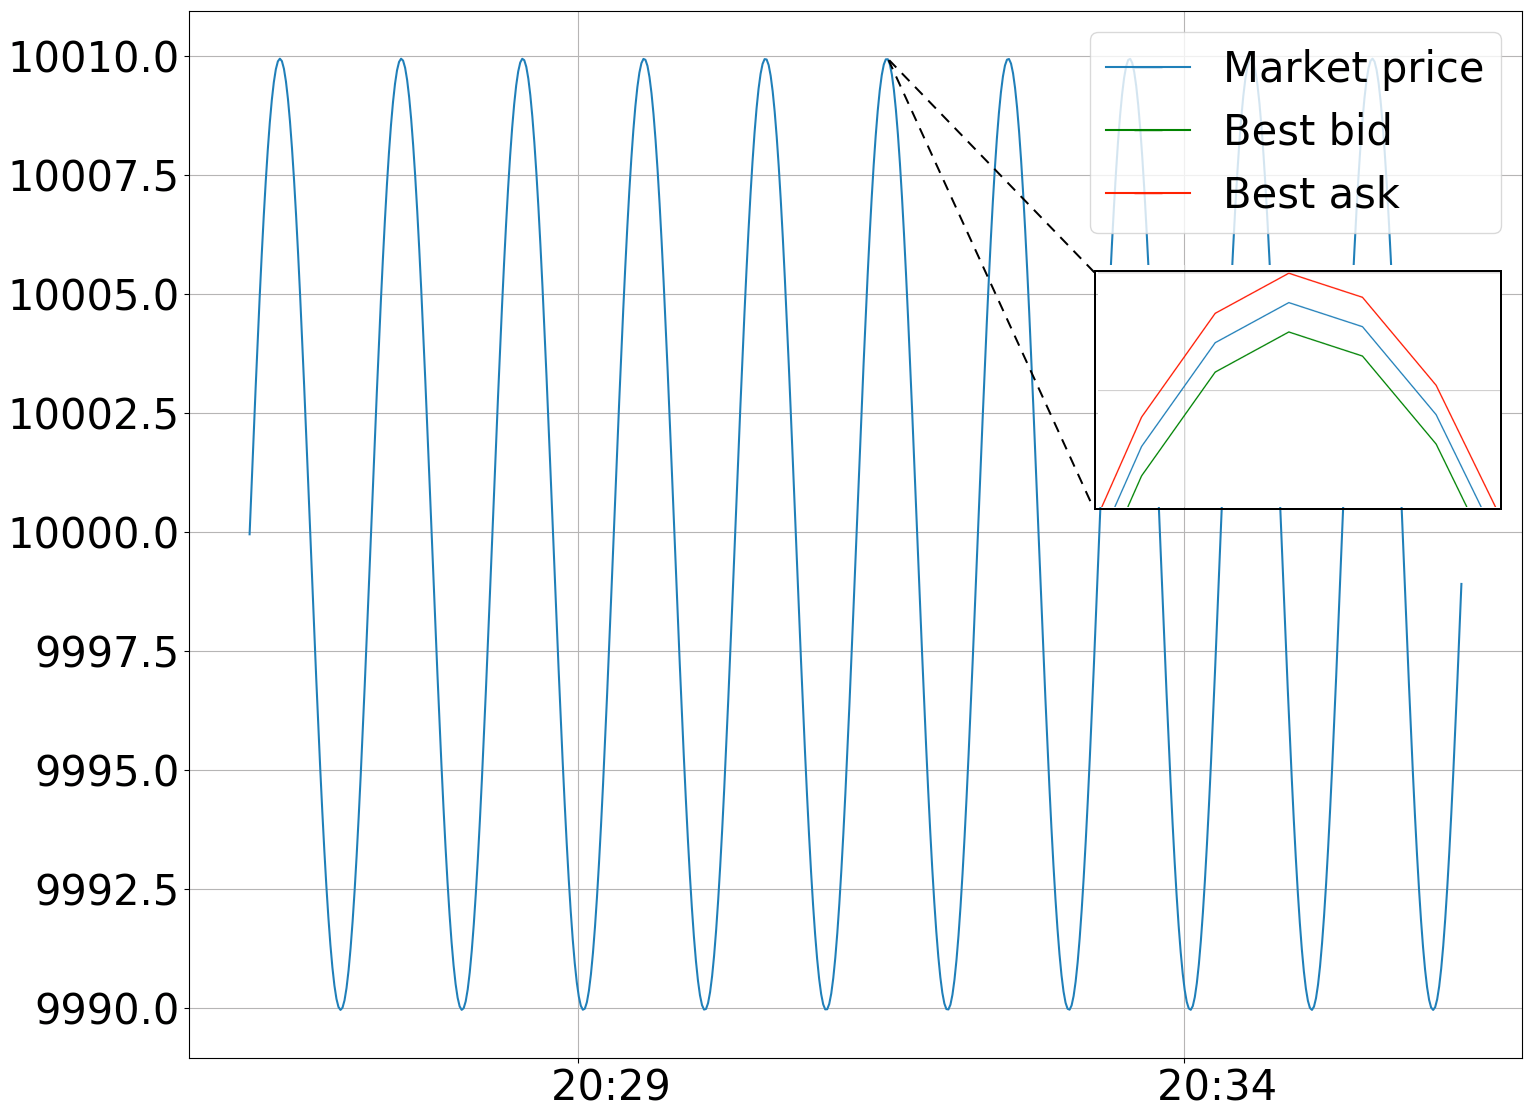
\includegraphics[width=\textwidth]{eval-limit-sine}
        \caption{Order book states configured according to sine function with $f=10$}
        \label{fig:eval-limit-sine}
    \end{subfigure}
    \caption{Artificial order books with duration of 10 minutes}\label{fig:eval-limit-artificial}
\end{figure}

The first example, as shown in Figure \ref{fig:eval-limit-down}, is a linear function which sets the market price to start at \$10,000 and end at \$9,940.
The price therefore falls by \$0.1 every second.
An agent should therefore realize that, when buying, the actions chosen should be negative ($a<0$) so that, in each step, a trade is transacted at the end of the time horizon at a much lower price.
The invariable reward after 100 seconds, for any state to start the order placement with, should therefore be \$10.0.
In contrast, the agent should realize that the loss when selling can be minimized by selecting a very positive action that results in an immediate sale.
The invariable reward should in this case be -\$0.10.

The second example, as shown in Figure \ref{fig:eval-limit-sine}, applies a sine function accross the order book states.
The frequency was set to 10, such that within one minute, at least one complete sine wave was generated with the amplitudes peaking at \$10,010.0 and \$9,990.0 respectively.
An agent is expected to learn to place limit orders according to the low and high peaks for buy and sell orders respectively.
The average reward for this example will not serve as an adequate measure of the policy since, depending on the state the agent starts at (that is the point in the amplitude), the optimal rewards can be different.
Instead, we relied on the volume-weighted average price directly and therefore expect the agent to buy close to \$9,990.0 and sell close to \$10,010.0.
\\
\\
Both artificial order book constellations were trained and tested with the DQN agent.
The configuration of the agent was chosen equivalent to the setup described in Section \ref{sec:eval-dqn} and a total of 5000 epochs were run in training and 1000 epochs in testing.
In the first example, which shows a clear downwards trend, the average reward during the backtest of buying assets resulted in \$9.45 and, for selling, in \$-0.10.
These results indicate that the agent was able to find a near-optimal policy.
The second example shows the multivariate sine wave that represents the order book and the average volume-weighted average price for buying was \$9,992.0 and, for selling, \$10,007.0.
This indicates that the agent was able to improve to an near-optimal policy with regards to the stationary development of the order book.

\section{Conclusion of the evaluation}

The evaluation procedure introduced and performed in this chapter showed that reinforcement learning techniques are indeed suitable for optimizing limit order placement for cryptocurrency markets.
The findings are summarized in Table \ref{tbl:analysis-conclusion}
First, we empirically estimated the potential improvements that can be achieved by placing orders at the the optimal limit level compared to an immediate sale or purchase using a market order.
We showed that, when the development of the market price is favorable to limit order placement, namely when the price is falling while buying or when the price is rising while buying, then the reward for the optimal limit order is expected to be significantly higher.
In situations where the market price is never favorable, then no improvement can be achieved and the optimal limit level is to cross the spread (a>0) which declares the order to become a market order that fulfills the demand to buy or sell immediately.
Subsequently, the Q-Learning agent was trained and tested without the knowledge of market data but with private variables (inventory and time horizon) only.
The average rewards achieved during a backtest have demonstrated that this agent was not able to take advantage of market price movements that were favorable to the order placement process.
However, the agent was able to reduce the costs when the market price development was  not favorable to either buying or selling assets.
In fact, the performance of the Q-Learning agent was the best of all considered agents, when it came to reducing the occurrence of unavoidable losses.
Subsequently, the DQN agent was evaluated under the independent application of two feature sets as well as two different types of action-value function approximators.
It has been shown that the application of feature II (a sequence of historical trades) results in a better policy than the application of feature I (a window of historical order book states).
Although the DQN was able to learn a policy that optimizes order placement when market conditions become favorable to buying or selling, the agent performed worse than the expected market order when conditions were not ideal.
Nevertheless, the DQN has ultimately achieved a performance which demonstrates the capability of placing and filling limit orders to a better price than what is offered at the market.
We have taken the better performing DQN setup, the DQN-CNN agent, and proceed further investigations.
Thereby we have shown that low dimensionality of the feature vectors have negative impact on the learning process, and so does a feature with very large dimensionality.
Furthermore, in order to understand why no policy could be learned that would constantly result in rewards better than the ones expected from using a market order, the actions taken by the DQN agent were analyzed.
It has been shown that 1) a wide spread between the best bid and ask price and 2) provided input samples of the market features prevented the agent from choosing actions which would fill an order at a better price than the market price.
Furthermore, artificially created order books were created and features derived therefrom.
It was shown that, in a scenario where short-term market fluctuations are absent and liquidity on the buyer and seller side is constantly provided, a deep reinforcement learning agent is able to find a near-optimal placement policy.
\begin{table}[H]
\centering
\begin{tabular}{l|l|l|l|l|l|}
\cline{2-6}
\textbf{}& \multicolumn{1}{c|}{\textbf{\begin{tabular}[c]{@{}c@{}}$\mathbb{E}$[Market \\ Order]\end{tabular}}} & \multicolumn{1}{c|}{\textbf{\begin{tabular}[c]{@{}c@{}}$\mathbb{E}$[Limit order]\\ (optimal)\end{tabular}}} & \multicolumn{1}{c|}{\textbf{Q-Learning}} & \multicolumn{1}{c|}{\textbf{\begin{tabular}[c]{@{}c@{}}DQN-CNN\\ (Feature I)\end{tabular}}} & \multicolumn{1}{c|}{\textbf{\begin{tabular}[c]{@{}c@{}}DQN-CNN\\ (Feature II)\end{tabular}}} \\ \hline
\multicolumn{1}{|l|}{\textbf{Buy (I)}}   & -0.05     & 15.20     & -1.17         & 22.06     & 31.92   \\ \hline
\multicolumn{1}{|l|}{\textbf{Sell (I)}}  & -27.70    & -27.70    & -21.34  & -39.26    & -25.15        \\ \hline
\multicolumn{1}{|l|}{\textbf{Buy (II)}}  & -1.06     & -1.06     & -1.04   & -2.26     & -3.56         \\ \hline
\multicolumn{1}{|l|}{\textbf{Sell (II)}} & -1.72     & 3.38      & -4.74         & 0.84     & 0.15    \\ \hline
\multicolumn{1}{|l|}{\textbf{$\Sigma$}} & -30.53     & -9.88      & -28.29         & -18.62     & {\ul 3.36}    \\ \hline
\end{tabular}
\caption{Summary of expected and achieved average rewards from empirical evaluations and reinforcement learning applications.}
\label{tbl:analysis-conclusion}
\end{table}
